% -*- mode: latex; coding: utf-8; fill-column: 72; -*-
% !BIB TS-program = biber
% !BIB program = biber

\documentclass[12pt]{umd-thesis}

\usepackage{graphicx}
\graphicspath{{images/}}

\usepackage{amssymb}
\usepackage{siunitx}
\sisetup{output-exponent-marker=\ensuremath{\mathrm{e}}}
\usepackage{multirow}

\usepackage[american]{babel}

\usepackage{csquotes}

\usepackage[
  backend=biber, style=unified,
  maxcitenames=3, maxbibnames=99]{biblatex}
\addbibresource{references.bib}
% just use a colon as the \postnotedelim
\renewcommand{\postnotedelim}{\addcolon}
\DeclareFieldFormat{postnote}{#1}
% use the Oxford comma
\DeclareDelimFormat{finalnamedelim}{%
  \ifnumgreater{\value{liststop}}{2}{\finalandcomma}{}%
  \addspace\&\space}
% a more sensible way to display the DOI
\DeclareFieldFormat{doi}{%
  \textsc{doi}:
  \ifhyperref
  {\href{http://dx.doi.org/#1}{\nolinkurl{#1}}}
  {\nolinkurl{#1}}}
%quirks of Yu'an:
\newcommand{\citealt}[1]{\cite{#1}}



%%for diagrams/ trees
\usepackage{tikz}
\usepackage{qtree}
\usepackage{tikz-qtree}
\usepackage{pifont} %to crossout movement path 
\usetikzlibrary{arrows,shapes, automata, positioning}
\usetikzlibrary{bayesnet}
\newcommand{\cmark}{\ding{51}}%checkmark
\newcommand{\xmark}{\ding{55}}%xmark

\usepackage{adjustbox}
\usepackage[mode=tex]{standalone}

\usepackage{xcolor}
\definecolor{darkred}{HTML}{B22613}
\definecolor{mygreen}{HTML}{C8DE9C}

\usepackage{gb4e}
\noautomath

\usepackage[colorlinks]{hyperref}
\hypersetup{%
  linkcolor=darkred,
  citecolor=black,
  urlcolor=cyan}

%%%%%%%%%%%%%%%%%%%%%%glossing
\usepackage{textglos}
\usepackage[
  block,
  nohypertypes={main} % option to pass to glossaries package 
]{leipzig}
\newleipzig{dou}{dou}{adverbial quantifier}
\newleipzig{sfp}{sfp}{sentence final particle}
\newleipzig{asp}{asp}{aspect marker}
\newleipzig{qpart}{q}{question particle}
\newleipzig{cl}{cl}{classifier}
%\newleipzig{ind}{ind}{indicative}
\newleipzig{int}{int}{interrogative}
\makeglossaries
%\newacronym{PMC}{PMC}{Principle of Minimal Compliance} %\gls{PMC}
\newacronym{dlearnerabbr}{SID}{Syntactically Informed Distributional Model} %\gls{}
\newacronym{plearnerabbr}{SPID}{Syntactically and Pragmatically Informed Distributional Model}
%%%%%%%%%%%%%%%%%%%%%personalized commands
\usepackage{verbatim}
\usepackage{float}
%gb4e hack
\newcommand{\bex}[1]{\begin{exe}\ex \label{#1}}
\newcommand{\eex}{\end{exe}}
\newcommand{\bxl}{\begin{xlist}\ex}
\newcommand{\exl}{\end{xlist}}

% semantics
\newcommand{\sv}[1]{\left\llbracket#1\right\rrbracket} % [[ ... ]]
\newcommand{\typ}[1]{\left\langle#1\right\rangle} 

%commands for style
\newcommand{\tit}[1]{\textit{#1}}
\newcommand{\tbf}[1]{\textbf{#1}}
\newcommand{\tsc}[1]{\textsc{#1}}
\newcommand{\tun}[1]{\underline{#1}}

%words
\newcommand{\ba}{\textit{ba}}
\newcommand{\ma}{\textit{ma}}
\newcommand{\twh}{\textit{wh}}
\newcommand{\dou}{\textit{dou}}
\newcommand{\twhi}{\textit{wh}-indefinite}
\newcommand{\hypos}{pragmatic syntactic bootstrapping hypothesis}
\newcommand{\diis}{declaratives, interrogatives, and imperatives}
\newcommand{\aqrs}{assertions, questions, and requests/commands}
\newcommand{\distlearner}{syntactically informed distributional learner}
\newcommand{\praglearner}{syntactically and pragmatically informed distributional learner}
\newcommand{\dlearnerabbr}{SID}
\newcommand{\plearnerabbr}{SPID}
\newcommand{\subhypos}{pragmatic bootstrapping hypothesis}
\newcommand{\mycode}{\url{https://osf.io/u9378/}}
\newcommand{\notdone}[1]{\textcolor{red}{#1}}
\newcommand{\revise}[1]{\textcolor{black}{#1}}


%%%%%%%%%%%%%%%%%%%%%title pages
\title{Learning to identify interrogatives and questions}
\author{Yu'an Yang}
\date{2022}

\cochair{%
  title={Professor}, name={Jeffrey Lidz}, department={Linguistics}}
\chair{%
  title={Professor}, name={Valentine Hacquard}, department={Linguistics}}
\committee{%
  {title={Professor}, name={Yi Ting Huang}, role={Dean's Representative}},
  {title={Professor}, name={Naomi Feldman}, role={}},
  {title={Professor}, name={Alexander Williams}, role={}},
  {title={Dr.}, name={Daniel Goodhue}, role={}}}



\begin{document}


\frontmatter

\begin{abstract}
  % -*- mode: latex; coding: utf-8; fill-column: 72; -*-

Languages tend to have three major clause types (declaratives, interrogatives, imperatives), dedicated to three main speech acts (assertions, questions, commands). However, the particular forms that these clause types take differ from language to language, and have to be learned. Previous experimental results suggest that by 18 months old, children differentiate these clause types and associate them with their canonical speech act. This dissertation investigates how children learn to identify different clause types and speech acts. 

To learn clause types, children need to identify the right categories of clauses (the ``clustering problem") and figure out what speech act they are canonically used for (the ``labeling problem"). I investigate the extent to which learners need to rely on pragmatic information (i.e., knowing what speech act a given utterance of a sentence is conveying), to solve not just labeling, but the clustering itself. I examine the role of pragmatics computationally by building two Bayesian clustering models. I find that morpho-syntactic and prosodic information are not enough for identifying the right clause type clustering, and that pragmatics is necessary. I applied the same model to a morphological impoverished language, Mandarin, and found that the model without pragmatics performs even worse. Speech act information is crucial for finding the right categories for both languages. Additionally, I find that a little pragmatics goes a long way. I simulate the learning process with noisy speech act information, and find that even when speech act information is noisy, the model hones in on the right clause type categories, when the model without fails. 


But if speech act information is useful for clause type learning, how do children figure out speech act information? I explore what kind of non-clause type cues for speech act information are present in the input. Even if children must rely on clause type information to figure out speech acts, they could have access to additional information that is unrelated to clause typing, but informative for recognizing speech act type. When speakers perform speech acts, because of the conventional functions of these speech acts on the discourse, the performance might be associated with certain socio-pragmatic features. For example, because of questions' response-elicitation function, we might expect speakers to pause longer after questions. If children are equipped with some expectations about the functions of communication, and about what questions do, they might be able to use these socio-pragmatic cues to figure out speech act. 

I explore two cues that could potentially differentiate questions from other speech acts: pauses, and direct eye gaze. I find that parents tend to pause longer after questions, and attend to the child more when asking questions. Therefore it is in principle plausible that there are some socio-pragmatic features that children can use, in addition to their growing knowledge of clause types to infer the speech act category of an utterance. This little bit of information about speech act could then be used to provide the information that the child needs in order to get the clause type clusters identified accurately.
%This dissertation We find (a) that a learner must have access to some pragmatic information in order to find the right clause types but (b) this learner can succeed with very limited access to pragmatic information. 

% Local Variables:
% TeX-engine: xetex
% LaTeX-biblatex-use-Biber: t
% TeX-master: "../main"
% End:

\end{abstract}

\maketitlepage

\makecopyrightpage

\begin{preface}
The work reported in this dissertation is highly collaborative. Chapter~\ref{chap:eng-cl} and Chapter~\ref{chap:man-cl}
report on joint work with Naomi Feldman, Valentine Hacquard, and Jeffrey Lidz; Chapter~\ref{chap:prosody} report on joint work with Thomas Schatz, Naomi Feldman, Valentine Hacquard, and Jeffrey Lidz; Chapter~\ref{chap:eng-sp} report on joint work with Daniel Goodhue, Valentine Hacquard, and Jeffrey Lidz. This work has also been supported by the National Science Foundation (Doctoral Dissertation Research Improvement grant~\#2140764 and NRT award~\#1449815).
\end{preface}

\begin{dedication}
\centering
To my parents, Chang Yang and Dr.~Jun Liu, for their unwavering support.
\end{dedication}

\begin{acknowledgments}
  Throughout graduate school, I must have played the scenario of writing this section of the dissertation a thousand times in my head; it always seems so far in the future that it almost seems fictional. I still can’t quite believe that, today is the day that I need to write this part of the dissertation. With sincere apologies to any that I may have forgotten, let me attempt to express my heartfelt thanks to everyone that has taken me to this point.
 
First, my deepest gratitude goes to Valentine Hacquard and Jeff Lidz. Before I even applied to UMD, everyone told me Valentine and Jeff together form a great advising team, and after working with them for five years, I can add my testament to this. Not only did they train me to become a better researcher and a careful thinker, but they were also my cheerleaders. They cheered me on whenever there was any breakthrough, no matter how small it was. I cannot count how many times I was about to give up on an idea, and only pushed through because Valentine and Jeff said “what are you talking about, this is great!” I feel so fortunate to have them as my mentors.
 
Thanks to my committee members, Naomi Feldman, Daniel Goodhue, Alexander Williams, and Yi Ting Huang. I was so nervous when I reached out to Naomi to ask for her help with building a computational model, because I barely understood anything from her class on cognitive modeling. But it turned out that I had nothing to worry about. Naomi was so kind and patient, even when she had to explain to me the extremely basic math for the nth time. Without her, I wouldn’t even dare to ask the ``how” question of learning, and half of this dissertation wouldn’t exist. She also connected me with people at the CLIP lab, which saved me so much time. Dan has always been a great mentor, and I had the fortune to both be a mentee, and a co-mentor. I learned so much about mentorship when we worked with a group of undergraduate students together. He also knows so much about prosody, and it was a lot of fun sitting in his office singing out utterances with him. Many thanks to Alexander for demonstrating to me how to be a careful thinker. He’d offer the most thoughtful and eloquent comments, often end with a joke that I fail to get (the Chomsky-Wittgenstein-Slab joke still puzzles me, no matter how many times he explains). I always wished I had recorded his comments at meetings, so I can write them down verbatim. Being his TA for his Philosophy of Language class was one of the most enlightening experiences for me as a semanticist.
 
I feel so lucky to have spent five years in such an amazing department. This community makes linguistics so much fun, and you know you are in the right place when you look forward to going to work every day. Thank you to Howard Lasnik, for reminding me how breathtakingly beautiful syntax can be, and for giving me the only A+ I’ve ever gotten; to Omer Preminger and Norbert Hornstein, for showing me how to think outside the box, and for reminding me to never lose sight of the big picture; to Colin Philips, for teaching me not to do experiments when you don’t have to; to Ellen Lau and Philip Resnik, for demonstrating to me how to make other cognitive scientists care about linguistics, and how to make linguists care about other fields of cognitive science; to Peggy Antonisse and Tonia Bleam, for teaching me how to teach in America; to Shevaun Lewis, for giving me so much good advice over the years and for puzzling over the PuffinMan data with me; and of course, to the incredible Kim Kwok, for always being so patient with me when I make mistakes filling out forms, and for teasing me for making them. I really enjoyed our daily chats at 9 in the morning that one year; too bad it stopped because of COVID.
 
Great mentors are hard to find, but I somehow found many over the years. I feel so unbelievably fortunate that I met Yang Xiaolu, Yang laoshi in Tsinghua. Thank you to Yang laoshi for introducing me to linguistics. It's hard not to fall in love with linguistics with Yang laoshi as the instructor. She also welcomed me to her lab, and encouraged me to ask questions and present ideas. Looking back, my ideas seemed so laughable. But Yang laoshi never laughed at them, she just helped me make them better. Even with all her guidance, she still made me feel that I had ownership over anything I was working on. Thank you, Yang laoshi!  
%always encouraged me to ask questions and present my ideas at conferences and lab meetings.  

I couldn’t remember which class I took with Roger Olesen, but it’s not important. In fact, I never thought of him as a teacher but as a friend. I want to thank him for always reminding me that the important things in life are your passion, your friends and family, and maybe Sichuan food.
 
Before UMD, I had the opportunity to spend a semester at UMass, and Angelika Krazter and Tom Roeper made this semester so special. Angelika opened the door of semantics for me. Still today when I run into a semantics problem, I always go back to her notes, and try to think like Angelika. I didn’t expect it, but Tom’s class, and our regular weekly chat quickly became my favorite time of the week at UMass. Brainstorming with Tom was the best. Before I came to UMass, I had my creativeness and passion beaten out of me, and was about to give up linguistics. Tom helped me find my passion and imagination back. Nothing was too crazy for Tom, and he never looked down on me when I presented him with a crazy idea. I can’t thank him enough for making linguistics enjoyable for me again. He was also extremely kind and supportive, and it has always been so great to run into him at acquisition conferences.
 
I only took one syntax class with Li Yafei, and one with James C-T Huang, but these two classes were so memorable and inspiring that I still think about them today. Before their classes, I didn’t really enjoy syntax, because I thought it was just about memorizing the right generalizations (yeah, horrifying, right?). They completely threw that idea out of the window. For the first time, I learned about \tit{how} to do syntax, and it has NOTHING to do with memorization. Thank you, Li laoshi, Huang laoshi!%Even though this dissertation is not a syntax dissertation, but without their \tit{dianhua} (I’m really not sure which English word would be the best equivalent, perhaps ``enlightenment”), I wouldn’t even be able to ask the questions I asked.

Thank you to Daniel Altshuler. I didn’t know it at the time when I met Daniel, but he was about to change my life. I still don’t understand why he decided to help me, but it might be just because Daniel is such a wonderful person. Thank you for looking out for me and Julian over the years, and can’t wait to see you again at conferences/summer schools!
 
I once heard that “Let’s work on this together!” is the academics’ way of saying “let’s start a band!” I’m so glad to have started bands with so many people over the years. Thank you to Mingming Liu, for teaching me about alternatives and exhausitivity so many times, and for tolerating my crazy questions. Working with you was very rewarding.  Thomas Schatz makes ASR less intimidating, and no matter what problem you want to solve, Thomas had written a script for it. Thank you for making it possible for me to have something related to prosody in this dissertation, and I’m really looking forward to continuing working on it to make it better. Nick Huang, you have always been my role model. It was so wonderful when you were still in the department to be able to just pop in your office and talk about linguistics, and I’m so glad we decided to officially work together last year. I hope we will continue our collaboration! And on that note, thank for introducing me to Aaron White and Zhendong Liu, and hope our project together will turn into a paper soon. Thank you to Tyler Knowlton. We tried to work together so many times but our experiments just keep getting mediocre results. I hope that one day one of our ideas will work! Thank you to Liao ChiaHsuan, hope we’ll pick up the \twh-indefinite project again someday! Liu Ying, you were my first non-supervisor collaborator, and we had to teach ourselves everything from lambda calculus to focus semantics, and it was the most rewarding experience. Gaor, I hope we get to work together again!
 
The acquisition lab at UMD is a special place. Jeff always says, it should be as professional as a dentist's office, but also as fun as a kindergarten (or preschool?). Indeed, I learned how to be a professional in the lab, and I had a lot of fun. The lab meeting was my favorite place to present my work, and I always walked out of 1108B with a better project. Thank you to my lab mates over the years: Laurel Perkins, Nick Huang, Mina Hirzel, Tyler Knowlton, Hisao Kurokami, Adam Liter, Iman Bou-Saboun, Jack Ying, and Katherine Howitt, for all the stimulating questions and great suggestions; and of course to Tara Mease, for teaching me how to be a good project manager. I also want to thank all of my RAs over the years: James Burns, Xiaoyu Yang, Ziqing Ji, Rin Gourianova, Luke Burger, Avni Gulrajani, Jae Yu, Eli Herbst, and Zhang Jiaobao, for making the project possible. I also got to work with James Burns, Xiaoyu Yang, Ziqing Ji, and Avni Gulrajani more closely in the past year, and it was such a wonderful experience. Thank you!
 
My sincere thanks to everyone at Haidian Xibeiwang Xuequ for helping me run my studies in Beijing from 2017-2019.  I want to especially thank Chen Shulan, Miao Zhibin, Zhang Xuening, and Zhao Xiaojing for their kind accommodation.
 
I’ve said this to so many people, but office 3416F is magical. Over the years, I’ve had the best officemates: Anouk Dieuleveut, Aaron Doliana, J\'essica Mendes, and Mina Hirzel. I don’t have any siblings, but you guys are like my sisters and brother.
 
Anouk, what can I say. You are like a sister to me. Together, we laughed, cried, and shared so many hugs and so much bread. It was so hard for me to say goodbye to you last year; just writing this filled my eyes with tears. I’m so glad we decided to keep working together via zoom, and it always makes me so happy to see your face. Thank you for everything!
 
Aaron, thank you for being my friend. You were the first person I met at UMD, and I’m so happy we got to share an office for three years (well, one and a half really because of COVID). Our “reading and Chinese takeout group of two” was indeed a good time. Thank you for always reminding me that you don’t have to stress yourself out as a graduate student. Thank you also for recruiting Divya and Myra to our hot pot party after Tyler and Zoe dropped out.

 
J\'essica, when I heard that you decided to come to Maryland, I was so happy. I almost immediately requested to have you as an officemate, but unfortunately, COVID delayed that for almost a year and a half. You made me laugh so hard. Thank you for being such a great friend, and I'm sorry I wasn’t so much fun when I started writing this dissertation. I hope we can keep in touch!
 
Mina, you are simply amazing. I admire you as a researcher and love you as a friend. Whenever I need to present something, I always ask myself, how would Mina do it? Your presentations and posters were always so clear, so beautiful, and so fun. But you are also so generous with your time and gave me so much great advice over the years. Hanging out with you (and occasionally Jad) every Sunday in your beautiful garden during COVID was the highlight of my week that year. Thank you for everything, and I can’t wait to go to all the good restaurants with you in Boston!
 
Many thanks to my cohort, Adam Liter, Hisao Kurokami, Jackie Nelligan, and Hanna Muller, and to Laura, Nima, Jon, and Aura. We had many good memories sharing an office in our first year, and later hanging out in Adam’s backyard. Laura, I’m so looking forward to going to karaoke with you and Katherine again!
 
I also want to thank my friends at UMD over the years whom I hadn’t shared an office with (but I wish I had): Paulina Lyskawa, Gesoel Mendes, Nick Huang, Ted Levin, Phoebe Gaston, Kasia Hitczenko, Laurel Perkins, Annemarie von Dooren, Tyler Knowlton, Laurel Whitfield, Jad Wehbe, Clara Cuonzoe, Luisa Seigun, Craig Thorburn, Allyson Ettinger, Anton Malko, Sigwan Thivierge, Masato Nakamura, Alex Krauska, Polina Pleshak, Joselyn Rodriguez, Nika Jurov, Lesli Li, Rosa Lee, Jack Ying, Yichi Xu, Chen Jingyi, Katherine Howitt, Zulfiyya Aghakishiyeva, London Dixon.
 
Thank you, Tyler and Zoe, for hosting so many hot pot parties. They were some of the best memories I had in Maryland. Remember that one time we had to wait until 11pm for the delivery of Asian groceries? It was definitely worth the wait. Also, thank you both for always answering my questions about cognition, and Tyler, hopefully one day one of our many efforts to work together will work out! Paulina, thank you for always checking in on me, it really made a difference. Annemarie, you have the best style, and the kindest smile, and hope we’ll get to see each other again sometime! Craig, thank you for helping me navigate the server, and for forgiving me when I accidentally flooded the \textsf{realspeech} directory (sorry again everyone). Anton, thanks for making R a little bit more understandable. Alex, I can’t believe we only found out about our shared love of the violin three months before I defend, and only got to play together once after my defense! But it was so much fun, and hope we will get to play together again sometime. Sig, you pulled the best prank, kudos! It still makes me laugh. Clara, thank you for always stopping by my office and giving me a hug! Allyson, sorry about bugging you about \tit{ba}, I didn’t understand how stressful you must have been; thank you for being so patient. Laurel, your work never fails to inspire me, and thank you for answering my many questions about them!
 
Thank you to my roommates in Maryland: Hallie Oines, Rana Karimpour, Beril Yalcinyaka, Julia Brown, and Erika Dömötör. I’ve been so lucky to have found the best roommates. Thank you for being so kind and understanding. Thanks to Zoe Schluter for introducing me to the house. Thanks to Patrick and Koki Smith for letting me live in their house for five years.
 
Thank you to Niki, Kelley, and Kathy at A Cat’s Life Rescue. Niki, I can’t imagine doing what you do. You are always so patient with my questions (most of the time the answer was “that’s normal”), always have the next kitty for me to foster, and never said no when I asked you to help a kitty. Thank you so much for coming to my house at 2am when Ally passed away to give me a hug. Seeing you and Phoenix always makes me happy. Kelley and Kathy, thank you for giving me some of the best foster babies (I miss Boss and Milo so much), and for always being there with medication and supplies when I need them. I couldn’t stop laughing because half of them have the word ``poop”, and the other half are adorable pictures of said poop (for those of you who are lucky enough to have never worried about cat poop: soft poop might be a sign for many health issues for kitties). I’m so grateful that all of you at ACLR gave kitties with all kinds of pooping- and non-pooping-related issues a chance.
 
I feel so lucky that I got into linguistics, because it’s such a great community. I made so many friends in this community, which makes going to conferences so much fun. Thanks to Rob Pasternak, Leah Chapman, Kimberly Johnson, Andrew Lamont, Zahra Mirrazi, Alex Göbel and Emma Nguyen-Göbel, Nathan Huang, Tom Maxfield, John Ander Mendia, Deniz Özyildiz, Mike Clauss, for making my semester at UMass feel filled with joy; thanks to Jess Law, Haoze Li, Yi-Hsun Chen, Mingming Liu, Beibei Xu, Hazel Mitchley, Shuhao Shih for a great time at Rutgers, and for making my first conference presentation less nerve-wracking; Thanks to Maxime Tulling, Daniel Altshuler, Yimei Xiang, Lucas Champollion, Ailis Cournane, Vera Zu, Wu Zhuang, Aaron White, Rachel Dudley, He Yuyin, Sun Yenan, Jackie Lai, Sherry Chen Yong, Xu Ting, Ji Yue, for all the great conversations and advice over the years, and for hosting me when I couldn’t afford hotels. The Barcelona ESSLLI connected me with so many wonderful people (including my future spouse), but a special thank you to Jenny Tan, Matt DeVilbiss, Markus Brenner, Anya Zaretskaya, Adam Kupś, Kuba Kozakoszczak, Lina Brixey. I will never forget all the delicious tapas, the beautiful breeze, and all the walks around Barcelona. Thank you my friends for reminding me how wonderful life could be.

 
I met some of my best friends in Hong Kong. Liu Ying, Jia He, Jess Law, Haoze Li, Ai Shu, Jia Li, Qun Li, Shi Xinyue, Guo Li, Yvonne Lee, Eunice Yip, and Xiaochun Hong, I cannot say thank you enough. I wouldn’t be able to survive those years without you guys.
 
Liu Ying, aka Gaor, thank you for everything. We were both in a tough situation, but you still decided to help me. You gave me hope and courage when I needed them the most. I hope you know how much your friendship means to me, and I don’t know how I can ever repay you. I miss you deeply, and hope I can see you and your baby soon!
 
Haoze and Jess, I don’t even know where to begin. When I felt like all the roads were blocked, you guys helped me find a way. I admire you both, and I'm so proud to call you my friends. I hope one day we get to have dinner again, and maybe Haoze’s cooking will be even better then!
 
He jia jie, you were the first one to ask me how I was doing. For that and for so many other things, I am forever grateful. Your laughter and optimism were contagious, and I’m so sorry we fell out of touch over the years. I really hope I get to see you again soon!
 
Ai Shu, Qunzi, and 2 Jia, thank you for always lending me sympathetic ears, and for tolerating me when I was being a selfish brat. I miss you guys, and hope we’ll get to \tit{dabianlu} again one day.

Li Guo, our bi-weekly syntax/prosody reading group was a lot of fun. Your knowledge of Classical Chinese always impresses me. Thank you for answering so many of my questions about the grammar of Classical Chinese.
 
Yvonne and Eunice, thank you for noticing that something was wrong. Special thank you to Eunice, for reminding me that there is always a way out. 
 
Thank you to my friends at Tsinghua: Shi Peipei, Qian Chen, Guo Jiabao (Carbo Kuo), Zhou Dong, Cao Tianchen, Zhu Qianyun, Li Meirong, Qian Yuzhu, Huang Binhuan, Lei Zhongxing, Zhang Wenxiu, Roger Olesen, Gwyneth Ho. Gwyneth, I’ve always admired your courage and determination. I hope one day I can hear your stories directly from you again, and not from the news. Thank you to Yang Nan, Shi Hanning, Yu Ning, for being such great friends.

Thank you to my first violin teacher, Ren Qifang. I didn't understand why you put so much effort on ear training, but it turns out to be the most valuable skill. It certainly comes in handy when I work on intonation in speech! Thank you for introducing me to the world of music. 

Thank you to my extended family in Chengde. Yeye, Laolao, Laoye, I miss you all. It still hurts that Nainai passed away while I was in America. I know she loved me, and would be proud of me. Thank you to Laoyi and Laoyifu, Dagu, Ergu and Ergufu, Laogu, Jiujiu and Jiuma for your support; thank you to my cousins Zhutianjie, Jin'aoge, Xinhe, Yang Rousi for your friendship (with lots of teasing of course). Because of graduate school, I missed so many important family moments, and I can only hope I can see you all soon. 

Thank you to my in-laws Anna and Bernd Schl\"oder, and my sister- and brother-in law Nikki, Lotte and Domi. I think about how lucky I am to have you guys all the time. Thank you for letting me play your violin! It's the best Christmas-birthday-graduation gift ever. Hope to spend Christmas with you soon!
 
I'm so lucky to have the best parents. Thank you for everything, Chang Yang and Dr.~Jun Liu! Ma, you are such an inspiration to me. You never back down from a difficult situation, and I hope you know how proud I am being your daughter. I want to tell everyone: “you see that fiercely brilliant woman, that’s my mom!” When my friends in the US told me the word “doctor” usually makes people think ``male,'' I laughed so hard because the best doctor I know is you. I learned how to be independent, thoughtful, and kind from you, and I hope you are ok with having another doctor in the family! Ba, sorry for always running away when you want to teach me something, but I hope you know how much I admire and love you. Thank you both for always being so loving, understanding, and open-minded. I didn’t know how valuable this is, until I saw how much my friends suffer because of their parents. I miss you both so much, and I hope I get to say \tit{wo ai nimen} in person soon.
 
Julian, thank you for sticking with me through graduate school. There have been so many ups and downs (writing being a huge down), but you are always there for me, sometimes with a funny story to make me laugh. I really couldn't have done it without you. Thank you for being such a great partner. The future may seem terrifying at times, but as our officiant said, we’ll “let love lead the way.” I love you and I like you.
 
 


\end{acknowledgments}

\tableofcontents\clearpage
\listoftables\clearpage
\listoffigures\clearpage
\begin{abbreviations}
  \renewcommand{\glossarysection}[2][]{}
  \printglossary[nonumberlist]
\end{abbreviations}



%%%%%%%%%%%%%%%%%%%%%%%%%%%%%%%%%%%%%%% main text
\mainmatter
% -*- mode: latex; coding: utf-8; fill-column: 72; -*-


\chapter{Introduction}
\label{chap:introduction}

We use language to perform various kinds of speech acts -- providing information, asking questions, making requests, etc. In any language, there are specific signals in the form of a sentence that indicates what speech act it is typically used for. In particular, cross-linguistically, languages tend to have dedicated clause types for the same three basic speech acts (\citealt{sz1985speechact, konig2007, aikhenvald2016, portner2018}, a.o.): declaratives are typically used for assertions (\ref{ex:intro:intro}a), interrogatives for questions (\ref{ex:intro:intro}b), and imperatives for commands (\ref{ex:intro:intro}c):

\bex{ex:intro:intro}
\bxl
That's Elmo. \hfill Declarative, Assertion
\ex Is that Elmo? \hfill Interrogative, Question
\ex Find Elmo! \hfill Imperative, Request
\exl
\eex


However, the surface formal features of these clause types differ greatly from one language to the next. For example, English declarative and interrogative differ in word order: auxiliary \tit{is} precedes the subject pronoun in the interrogative sentence (\ref{ex:intro:intro}b) but not in declaratives (\ref{ex:intro:intro}a); Mandarin interrogatives and declaratives do not differ in word order, but instead, interrogatives are marked by the sentence final particle \tit{ma}, as evident in (\ref{ex:intro:man}a-b): 

\bex{ex:intro:man}
\bxl
\gll Zhe shi Elmo.\\
This is Elmo\\
\trans ``This is Elmo." \hfill Declarative
\ex 
\gll Zhe shi Elmo \tbf{ma}?\\
This is Elmo \Sfp\\
\trans ``Is that Elmo?'' \hfill Interrogative
\ex 
\gll Zhizhi Elmo!\\
Point Elmo\\
\trans ``Point at Elmo!'' \hfill Imperative
\exl
\eex

Therefore, children need to figure out the language-specific surface formal features of their clause types. In this dissertation, I ask how children learn the surface signals associated with the clause types while learning to identify the speech acts that these clauses express. There are several problems that they must have solved.

\section{The problem with clause types}

Clause types are grammatically defined classes of sentences (see \cite{portner2018} for a recent review)\footnote{For some, clause types are form-meaning pairings (\cite{sz1985speechact, ginzburgsag2000interrogative}). We'll come back to this terminological difference in the next chapter, but in this dissertation, I take clause type as a grammatical concept, sentence mood (or sentential force) as the mapping of form and meaning, and speech act as either the act that speaker performs with a sentence, or the conventional effects of a sentence on the discourse.} 

The clause type information is often analyzed as related to  phonetically null morphemes like Q (\cite{katzpostal1964, baker1970int}) or features of $C^{0}$ (e.g. [\textpm int, \textpm imp], cf. \cite{langacker1974q, chomsky1995minimalist, rizzi1997, rizzi2001int, chomskylasnik1977, cheng1991,platzack1997imp,akmajian1984clausetype}). What learners need to figure out is then which sentences have the [+int] value and which ones take the [-int] value (or whether the Q morpheme is present). For example, while (\ref{ex:intro:cluster-base}) and (\ref{ex:intro:cluster}a) are two different strings, the learner needs to recognize that they share the same feature when it comes to clause types, frequently analyzed as a [+int] feature on $C^{0}$. They also need to recognize that even though (\ref{ex:intro:cluster}a) and (\ref{ex:intro:cluster}b) share the same lexical items, their $C^{0}$ are marked with different features: [+int] for the former, and [$-$int] for the latter.%So the child must come to treat (\ref{engcl:cluster}) and (\ref{engcl:cluster}a) alike (because of subject-aux inversion triggered by [+int] in $C^{0}$) and distinct from (\ref{engcl:cluster}b). 




\bex{ex:intro:cluster-base}
Do you want a cookie?
\eex
\bex{ex:intro:cluster}
\bxl{}
Is that Elmo?
\ex
That’s Elmo!
\exl
\eex


But this feature [\textpm int] is an abstract feature and thus cannot be directly read off from the surface string, so the learner is left with the task of inferring which feature is on $C^{0}$ from surface form. To achieve this, they need to find the right way to cluster of sentences in the language. In other words, when given a new sentence (\ref{ex:intro:cluster-base}), they should be able to put it in the same clause type category as (\ref{ex:intro:cluster}a) and not (\ref{ex:intro:cluster}b). I will refer to this problem as the \tbf{clustering problem}. 

Solving this problem isn't straightforward, as clause type features of $C^{0}$ do not have a one-to-one mapping with morpho-syntactic properties in the surface form of sentences. For example, as discussed above, the [+int] feature of $C^{0}$ in English is usually associated with the raising of auxiliaries, resulting in subject-aux inversion. But in embedded clauses, [+int] does not trigger the raising of auxiliaries, and consequently, we won't see subject-auxiliary inversion in these interrogative clauses: 

\bex{ex:intro:eng-embed}
Mary wonders \tun{whether Ann can hug Elmo.}
\eex
\bex{ex:intro:eng-can}
\bxl
Ann can hug Elmo.
\ex Can Ann hug Elmo?
\exl
\eex
As shown in (\ref{ex:intro:eng-embed}), the auxiliary \tit{can} and subject \tit{Ann} of the embedded interrogative have the same word order as the matrix declarative sentence (\ref{ex:intro:eng-can}a).


Conversely, some morpho-syntactic properties typically associated with [+int] could also appear in other settings. For example, [+int] in Mandarin could be expressed by having a \twh-phrase in the sentence. But, [$-$int] sentences could also have \twh-phrases, where these phrases are interpreted as indefinites like English \tit{any/a}. As a result, a string like (\ref{ex:intro:m-whamb}) could be either an interrogative (interpretation a) or a declarative (interpretation b). 


\bex{ex:intro:m-whamb}
\gll Xiaoxiao mei 	chi 	\tun{shenme} dongxi\\ 
Xiaoxiao \Neg{} 	eat	what	things\\
a.	``What didn’t Xiaoxiao eat?''	\hfill Interrogative \twh\\
b.	``Xiaoxiao didn’t eat anything.''		\hfill Indefinite \twh
\eex

Therefore, learners need to infer the abstract clause type feature of sentences, but they might not see the morpho-syntactic properties typically associated with clause type feature, or the property that they do see misaligns with the actual clause type feature of the sentence.

Another related problem is that, learners have to learn their language-specific way that [+int] are expressed. A case in point: in English, the subject and verb switch their canonical order in interrogatives (\ref{ex:intro:intro}a-b), but Mandarin employs sentence final particles for interrogatives (\ref{ex:intro:man}a-b).  

%%%%%%%%%%%%%%%%%%%%%%%%%
In the principle and parameter approach, a way to solve this cross-linguistic variation problem is to propose a parameter that covers all the variations. The learners are given choices for how to type a clause (i.e. assign [+int] or [-int] to $C^{0}$) by setting the value of a parameter. For example, \textcite{cheng1991} proposes the Clause Typing Hypothesis:

\begin{quote}
Every clause needs to be typed. In the case of typing a \twh-question, either a \twh-particle in $C^{0}$ is used or else fronting of a \twh-word to the Spec of $C^{0}$ is used, thereby typing a clause through $C^{0}$ by Spec-head agreement. \hfill \textcite[p.29]{cheng1991}

\end{quote}


According to this hypothesis, \twh-movement languages such as English assign a [$+$int] ([+wh] in Cheng's terminology, but it includes all interrogative clauses) value to the $C^{0}$ of sentences like (\ref{ex:intro:cheng-eng}) by moving the \twh-phrase to clause-initial position.\footnote{Note in other theories of [+int] and \twh-movement (e.g. \cite{chomsky1995}), \twh-movement does not assign [+int] to $C^{0}$, but is motivated by [+int]. } Meanwhile, \twh-in-situ languages achieve the same goal by utilizing a \twh-particle, \tit{ne}, as illustrated in (\ref{ex:intro:cheng-man}).

\bex{ex:intro:cheng-eng}
Who can Ann hug?
\eex
\bex{ex:intro:cheng-man}
\gll
Ann neng baobao shui (ne)\\
Ann can hug who \Sfp\\
\trans ``Who can Ann hug?''
\eex

%Putting aside the controversy about \twh-particles (cf. \cite{bruening2007wh, yangyang2018}), 
As \twh-particles are optional in many in situ languages, Cheng associates a particular learning strategy with this hypothesis: learners use the presence of polar question particle (e.g. \tit{ma} in Mandarin) to learn

since languages have two ways of realizing [+int], learners identify the abstract clause type feature by observing whether their language allows \twh-particles. 


In this dissertation, we explore a different way of solving the clustering problem, namely whether they can use their ability to track the distribution of certain features. Specifically, learners need to use pragmatic information (i.e. the speech act of the sentence), in conjunction with observations of distributions of morpho-syntactic features in the surface form of sentences, to infer clause type clusterings. We will return to this hypothesis later. 



After identifying the clusters, learners need to determine the canonical function of each cluster in the system. That is, after clustering sentences into three categories, children still need to learn which one of these clusters is the interrogatives, which is the declaratives, and which is the imperatives. We will refer to this as the \tbf{labeling problem}. To break into this labeling problem, the learner might need to use the function of the utterance -- the speech act information. As many have noticed, clause types are systematically related to the speech act of a sentence (\cite{katzpostal1964, sz1985speechact}). If the learner observes that a cluster of sentences is more frequently associated with questions, they might be able to label this cluster of sentences as the one whose canonical function is asking questions (i.e.\ interrogatives), and similarly for declaratives and imperatives. 

But the mapping between speech acts and clause types is not one-to-one, as we will see below.





%Some proposals (e.g. ) for clause type features in $C^{0}$ even state that this feature is the syntactic representation of .


\section{The problems with speech act}
%indirect speech act here
while clause types constrain the illocutionary force of an utterance, the mapping between them is not inviolable. Some speech act categories can be expressed by more than one clause types, and vice versa (\citealt{searle1975tax}, \citealt{searle1976class}, \citealt{bachharnish1979}, \citealt{levinson1983},\citealt{searlevanderveken1985}, \citealt{portner2018}, \citealt{starr2014}, \citealt{murraystarr2020} a.o.). For example, interrogatives can express assertions, questions, requests/commands (\ref{eng-cl:q-all}); and questions can be expressed by \diis{} (\ref{eng-cl:int-all}).
\bex{eng-cl:int-all}
Interrogatives can express all kinds of speech acts:
\bxl Is it snowing? \hfill Question
\ex Aren't you sweet. \hfill Assertion
\ex Can you pass the salt? \hfill Request
\exl
\eex

\bex{eng-cl:q-all}
Questions can be expressed by all kinds of clauses:
\bxl
Is it snowing? \hfill Interrogative
\ex It's snowing? \hfill Declarative
\ex Tell me if it's snowing! \hfill Imperative
\exl
\eex



 %So how do children figure out the canonical mapping between the formal features of interrogatives and their conventionalized function as questions?  
Meanwhile, the learning of speech acts also have the same clustering and labeling problem. Children also need to figure out that the utterance they just heard is a question that needs response, and not an assertion. 


Despite all the challenges, infants seem to have figured out clause types and speech acts by 18 months old, as we will see in the next chapter. How do infants learn to identify clause types and speech acts, especially interrogatives and questions?

\section{Pragmatic syntactic bootstrapping hypothesis}
\label{sec:intro:prag-syn-bootstrap}

I hypothesis that children jointly learn the speech act and clause type categories from observations of pragmatic, prosodic, and syntactic features of utterances. On the one hand, children learn to identify questions by exploiting the prosody of the utterance and the pragmatic features of the utterance (such as the social function of the utterance and the social attentional behavior of the speaker); on the other hand, they learn to identify interrogatives by exploiting the syntactic features of the sentence. Crucially, however, learning to identify questions and learning to identify interrogatives are also mutually constrained: children could use speech act information to learn the makeup of interrogative clauses in their language, and use clause type information to learn the pragmatics of questions. 

In this dissertation, I test a weaker version of this hypothesis with a focus on clause type identification:

\begin{quote}
Infants learn to identify abstract clause type categories with the speech act information, in conjunction with observations of morpho-syntactic features in the surface form of sentences.
%Infants need to use the speech act information to cluster sentences into the three major clause types. 
\end{quote}

%To test this hypothesis, a necessary first step is to establish a systematic, empirical picture on the information contained in the input data that children receive. What clause types are used, and with what function? What features of the context in the input might reveal a questioning act?  To this end, we propose two studies: Study~1 examines speech to English-speaking children and Study~2 examines speech to Mandarin-speaking children. In both studies, we will make use of data from existing corpora of parent-child interactions and annotate each utterance for a theoretically motivated set of features, encompassing a sentence’s syntactic features as well as the corresponding utterance's prosodic and social pragmatic features. In addition to building an annotated dataset of the input, we want to model this learning process computationally to understand \tit{how} children can use the information from their input. Study 3 provides a proof of concept for the \hypos{} for the acquisition of questions and interrogatives.

To get us one step closer to the full-fledged version of \hypos{}, I also explore what kind of non-clause type cues are present in infants' interaction with parents that will allow them to cluster speech act categories. 

Previously, this \hypos{} where pragmatics and syntax are mutually constraining has been proposed for the learning of attitude predicates (\citealt{lewis2017think, dudleyetal2018, hacquardlidz2018}), modals (\citealt{dieuleveut2021}), and quantifiers (\citealt{knowlton2021}). We argue that the learning of interrogatives and questions is another case where the learner need to exploit the correlation between pragmatics and syntax to succeed.  







\section{Discussion and roadmap}
\label{sec:intro:roadmap}

Learning to identify clause types and speech acts is important for early language acquisition. The acquisition of various basic syntactic phenomena like argument structure, word meanings, and basic word order, might be aided by an ability to distinguish declarative clauses from other clause types (\citealt{pinker1984, pinker1989, gleitman1990, frankgoldwaterfrank2013, perkins2019} a.o.), as identifying clause types is helpful in explaining word order variability and the distribution of missing arguments. There is also reason to believe that learning this basic distinction is necessary for the acquisition of more complex structural properties, such as the semantics of clause-embedding verbs such as \tit{think}, \tit{know} and \tit{wonder}. Learning the clause type distinctions may help children notice the subcategory distinction between these three types of verbs and then could aid in learning related semantic notions like veridicality (\citealt{white2015diss, lewis2017think,dudley2017,hacquardlidz2018}). As for speech acts, they are not only crucial for toddlers' language learning (\citealt{ninio1980, hoff1985cds,yoder1994,rowland2003cdswh, valian2003cds, rowe2017wh, gaudreau2021question} among many others), but also for cognitive development in general (\citealt{hohmann1995educating} among many others). 

This dissertation investigates how infants come to identify clause types and speech acts. This dissertation is organized as follows. Chapter~\ref{chap:background} examines the developmental trajectory of speech acts and clause types, especially questions and interrogatives. As we will see, English-acquiring infants as early as 18 months seem to have already sensitive to the distinctions between different clause types and speech acts, and seem to understand the mapping between questions and interrogatives. The same holds for infants acquiring other languages as well, even though we have less evidence. Our question then is, how do 18-month-olds learn to figure out clause types?

Chapter~\ref{chap:eng-cl} looks at how English-acquiring 18-month-olds could have solved the problem. Specifically, is information from syntax enough for children to find the right three clause type categories, or do they need pragmatic information like the speech act of the sentence to find the right clustering? I build two computational models to address this question, a \distlearner{} (\dlearnerabbr{}), and a \praglearner{} (\plearnerabbr{}). These two learners both need to infer the abstract clause type, but \dlearnerabbr{} draws inferences from syntactic information alone while \plearnerabbr{} uses both syntactic and pragmatic information. I use a corpus study to first provide a quantitative description of the type of input that infants get, and use the resulted annotated dataset as input for the computational models. I find that pragmatic information is indeed important for solving the clustering problem: without the speech act information, \dlearnerabbr{} cannot find the right clause types. Additionally, a little pragmatics goes a long way, as  even if 80\% of the pragmatic information is noise, it still improves the learner's performance. 

Chapter~\ref{chap:man-cl} applies the same methodology to another language, Mandarin. Mandarin-acquiring infants figure out the clause types of their language around the same age as English-acquiring infants, but the two languages employ different morpho-syntactic features for clause typing. How do Mandarin-acquiring infants solve the problem? Do they also need pragmatic information? I compare the same two learners, and found that pragmatics information is crucial for identifying Mandarin clause types as well.

But so far, we are operating under the assumption that infants have speech act at their disposal. How do they figure out the speech acts of parents' utterances? Of course their knowledge of clause type might help, but are there signals from other sources? Chapter~\ref{chap:eng-sp} explores cues from prosody and parents' behavior that might help infants identify questions. Chapter~\ref{chap:discussion} concludes the dissertation.
 
% Local Variables:
% TeX-engine: xetex
% LaTeX-biblatex-use-Biber: t
% TeX-master: "../main"
\chapter{Background}
\label{chap:background}

This dissertation investigates how children figure out the clause types of their language, on the basis of their input. In this chapter, I review what we already know from the existing literature on (1) the target knowledge, namely the formal properties of clause types and speech acts and their analyses in the formal literature; (2) children's understanding of clause types and speech acts, and the linguistic and pragmatic capacities that they can draw from early in development, and what we know about the kinds of speech acts and clause types children are exposed to. I will come back to English and Mandarin-acquiring children's morpho-syntactic knowledge in Chapter~\ref{chap:eng-cl} and Chapter~\ref{chap:man-cl}.

\section{Theories of clause types, sentential force, and speech acts} \label{sec:bg:theory}


\subsection{Speech acts and force} \label{sec:bg:theory:speech}

Frege observes that it is possible to express a thought without judging it to be true -- that considering a particular claim and judging it to be true are different things altogether. In asking a polar question like \tit{Is it raining?} one is not judging anything to be true. But in answering \tit{Yes }or asserting the declarative sentence like \tit{It is raining}, one does. Nevertheless, \tit{Is it raining?} and \tit{It is raining} have something in common: they have the same content, or as Frege puts it, they contain the same \tit{thought}. From this observation, he derives the influential distinction between \tit{content} and \tit{force}. The following passage from \tit{Der Gedanke} makes this distinction clear:

\begin{quote}
    

An interrogative sentence and an assertoric one contain the same thought; but the assertoric sentence contains something else as well, namely assertion. The interrogative sentence contains something more too, namely a request. Therefore two things must be distinguished in an assertoric sentence: the content, which it has in common with the corresponding propositional question; and assertion. The former is the thought or at least contains the thought. So it is possible to express a thought without laying it down as true. The two things are so closely joined in an assertoric sentence that it is easy to overlook their separability. 

$\,$\hfill \cite[62]{frege1918thought}, Translated by Peter Geach and R. H. Stoothoff
\end{quote}

That is, the polar question \tit{Is it raining?} and the assertion \tit{It is raining} both contain the same thought, namely \tit{whether it is raining.}  But \tit{Is it raining?} presents this thought with questioning force and \tit{It is raining} presents it with assertoric force. By presenting a thought with assertoric force, one expresses that one judges the thought to be true. But there are other ways of presenting the same thought, for example with questioning force.\footnote{However, Frege argues that the question of truth does not arise for sentences expressing commands, requests, wishes etc., so even though a sentence expressing request have sense, its sense is not a \tit{thought}.}

The idea of ``force'' is further developed by \textcite{austin1975things} in his work on speech acts. The core observation is that, utterances may have a variety of forces, not just asserting and questioning, but also promising, declaring, warning, marrying, naming and so on. According to Austin, the same sentence can in principle be used with a broad variety of forces:

\begin{quote}
    
We may be quite clear what \tit{Shut the door} means, but not yet at all clear on the further point as to whether as uttered at a certain time it was an order, an entreaty or whatnot. What we need besides the old doctrine about meanings is a new doctrine about all the possible forces of utterances.

\hfill \cite[251]{austin1975things}
\end{quote}

This new doctrine is to categorize utterances primarily by what one \tit{does} with them, rather than what they \tit{mean}. His analysis of what one does with an utterance happens on three levels: the locutionary act (the act of speaking), the illocutionary act (the act done through speaking, e.g. informing, warning, requesting), and the perlocutionary act (the by-product of producing the utterance). Let’s walk through an example with these three levels. If we utter a sentence like \tit{The campus is closed tomorrow}, the locutionary act is that the speaker utters these very words; the illocutionary act is that the speaker informs the addressee of the news about campus shutdown, and (at least one of) the perlocutionary acts here is that the speaker is changing the addressee’s plans about coming to campus tomorrow. The illocutionary act is of particular interest, as it is the speaker’s intent to inform by producing the utterance. To be more precise, according to Austin, the speaker and hearer are engaging in a conventional procedure of information sharing in which performing a certain locutionary act \tit{is} to perform a certain illocutionary act. The locutionary act has its illocutionary force in virtue of being a part of this conventional procedure. The utterance has informing force by convention.

Austin is in particular interested in developing a taxonomy of speech acts. He focuses his attention on categorizing \tit{speech act verbs}: the verbs that can be explicitly used to invoke a particular convention when appearing in the same sentence as the word \tit{hereby}. For example, one invokes the procedure of information sharing (i.e. one makes explicit that one is performing the illocutionary act of informing) by saying \tit{I hereby inform you}. Note that not all verbs with a communicative meaning are speech act verbs. For example, it is odd to say \tit{I hereby surprise you.} So, in Austin's taxonomy, \tit{surprising} is not an illocutionary force, but \tit{informing} is.

\textcite{searle1969} points out that there is no reason to believe that the verbs of English (or any other language, for that matter) exhaust the illocutionary forces. There could be illocutionary forces that do not correspond to a verb. However, Searle agrees with Austin that speech acts, and in particular their illocutionary forces, involve certain social conventions and constitutive rules. Searle moreover follows \textcite{grice1957meaning} in stressing the role of the speaker’s intention to perform a certain act and to be recognized as performing this act. Specifically, %the intention recognizable, according to Searle, is by  how the locutionary act is performed in accordance to certain conventional rules:

\begin{quote}
In the performance of an illocutionary act, the speaker intends to produce a certain effect by means of getting the hearer to recognize his intention to produce that effect, and furthermore, if he is using words literally, he intends this recognition to be achieved in virtue of the fact that the rules for using the expressions he utters associate the expressions with the production of that effect.\\
\hspace*{\fill} \hfill \cite[259]{searle1969}
\end{quote}

\textcite{searle1976class} then gives the following broad categorization of speech acts by what they are used to achieve:

\bex{spact:searle-tax}
\bxl
assertives = speech acts that commit a speaker to the truth of the expressed proposition
\ex directives = speech acts that are to cause the hearer to take a particular action, e.g. requests, commands and advice
\ex commissives = speech acts that commit a speaker to some future action, e.g. promises and oaths
\ex expressives = speech acts that express on the speaker's attitudes and emotions towards the proposition, e.g. congratulations, excuses and thanks
\ex declarations = speech acts that change the reality in accord with the proposition of the declaration, e.g. baptisms, pronouncing someone guilty or pronouncing someone husband and wife
\exl
\eex

Like Frege, Searle also draws a strict distinction between \tit{force} and \tit{content}. However, there are some significant differences between Frege’s and Searle’s views on the distinction. For Frege, content is what the sentence radical expresses (e.g. what’s in common between a declarative and a polar interrogative). But for Searle, expressing a content is an act, and he does not see how ``sentences could perform acts'' (\cite[257]{searle1976class}). Rather, acts are performed by speakers. Thus, speakers perform illocutionary acts, and (most of) illocutions involve the expression of a content.\footnote{Searle explicitly mentions that there are illocutionary acts without contents, such as \tit{Ouch!} or \tit{Hurrah!}} The content of an illocutionary act is the proposition that the speaker expresses by uttering a particular sentence. Nevertheless, of course, which sentence the speaker utters (and how they utter it) influences what the content and the force of the illocutionary act are. 

According to Searle, sentences have a proposition-indicating element and a function-indicating element that in later work he calls the \emph{illocutionary force indicating device} (IFID) of a sentence (\cite{searle1976class}). For him, IFIDs are formal features of a sentence. For example, English IFIDs include word order, stress, intonational contour, punctuation, the mood of the verb, and certain lexical elements (notably, Austin’s speech act verbs). However, he also notes that in many circumstances the context alone is sufficient to indicate force, so IFIDs do not always need to be explicit (\cite[257]{searle1976class}). 


%The possibility of indirect speech acts exacerbates this issue further, as \tit{The campus is closed} could also be an indirect answer to a question like \emph{Are you going to class?}, or a request to hand over a key, or a plea to extend a homework deadline. 



This way of associating the formal features of a sentence with illocutionary force leads Searle to the discussion of \tbf{indirect speech acts}. These are sentences that ``contain the illocutionary force indicators for one kind of illocutionary act can be uttered to perform, in addition, another type of illocutionary act'' (\cite[168]{searle1975indirect}). For example, subject-auxiliary inversion is an IFID indicating the questioning force, but a dinner guest uttering \tit{Can you pass the salt?} is using the sentence to perform a requesting act. Searle argues that the speaker performs the questioning act by way of performing the requesting act; the questioning force is the ``secondary'' and ``indirect'' illocutionary act and the ``literal'' meaning of the utterance, whereas and the requesting force is the ``primary'' act and ``nonliteral'' meaning of the utterance (\cite[170]{searle1975indirect}). 

This tension between the form of the sentence and the intention of the speaker seems to be a problem for Searle. On the one hand, Searle concedes that ``the utterance has two illocutionary forces,'' questioning and requesting, because ``the speaker intends to produce in the hearer the knowledge that a request has been made to him, and he intends to produce this knowledge by means of getting the hearer to recognize his intention to produce it'' (p.168); on the other hand, he argues that the sentence itself, and sentences like this one, ``do not have an imperative force as part of their meaning'' (p. 172), because there is no IFIDs in the sentence related to the imperative force, and the same sentence could be used to not convey the imperative intention. Searle's solution is to argue that even though there is no IFID for the imperative force, the hearer can identify an ulterior illocutionary point beyond the illocutionary point contained in the meaning of the sentence (\cite{searle1975indirect}), and use recognizing the existence of this ulterior illocutionary point to infer the requesting force. An ``illocutionary point'' refers to ``the point or purpose of a type of illocution'' (\cite{searle1975tax}), which the hearer can infer with principles of conversations.   

\textcite{searlevanderveken1985} then pursue the project of developing a taxonomy for all possible illocutionary forces. They suggest that each possible illocutionary force can be defined as a septuple of values, each of which is a ``setting'' of a value within one of the seven characteristics of illocutionary acts: the illocutionary point, its degree of strength, the mode of achievement, the content conditions, the preparatory conditions, the sincerity condition, and the degree of strength of the sincerity condition. It follows, according to this suggestion, that two illocutionary forces F1 and F2 are identical just in case they are characterized by the same setting of these seven values. 

While it is true that there are problems with this specific set of criteria that \textcite{searlevanderveken1985} proposed (e.g. it seems that ``illocutionary point'' is just another name for illocutionary force), the broader problem with the Austianian-Searlean approach seems to be that there is a general pattern that speakers can use sentences to perform all kinds of acts, and it is very hard to pinpoint the exact act that is performed in a specific case, no matter how many criteria we propose. This problem already manifests in some way in our previous illustration of Austin's theory with the utterance \tit{The campus is closed}. When talking about the example, it seems natural to say that the illocutionary act is informing, but couldn’t we say just as well that the speaker intends to produce an effect of warning in the hearer with the sentence? Or an effect of lamenting? Or all of the above? This problem makes it extremely difficult to implement their taxonomy of speech acts. As many examples (such as \tit{The campus is closed}) do not come with an explicit speech act verb like \tit{inform} or \tit{warn} (e.g. in \tit{I’m warning you that} \ldots), it  is almost impossible to discern the intended effect to the level of fine-grainedness given by an Austinian taxonomy of speech act verbs or a Searlean taxonomy of possible acts. As any group of annotators attempted to label corpus data using the Austinian-Searlean methods would tell you, applying these definitions to specific examples is extremely difficult and achieving any sort of inter-annotator agreement in the task of classifying speech acts according to such a taxonomy is next to impossible.\footnote{An unfortunate consequence of the multitude of illocutionary forces that one may attribute to the same utterance is that, in order to boost inter-annotator agreement, annotation schemes sometimes blend formal categories with functional categories. For example, in the schemas discussed in \textcite{ninio1994} and \textcite{dialogact}, \twh-interrogative and polar interrogatives are included in the labeling.} 

At the same time, discarding the link between IFIDs and force because of the existence of indirect speech acts (e.g. as suggested by the radical pragmatics approach, \cite{atlaslevinson1981, levinson1983}) seems to miss this important association between form and function. As we have seen in Chapter~\ref{chap:introduction}, languages tend to have \diis{} dedicated to \aqrs{}. Ignoring this universality seems to miss an important generalization in language. While it is true that there is a mismatch between the conventional effects linked to polar interrogatives and the speech act performed by the speaker in the indirect speech act \tit{Can you pass the salt?} example, the very fact that we intuitively interpret the sentence as a question suggests that we probably do not want to take form out of the equation.

At this point, it appears fruitful to attend not to the fine distinctions of Austinian speech act verbs, nor to the distinctions of Searle and Vanderveken’s metaphysics of action, but rather to how utterances affect the context they are made in (\cite{hamblin1971, stalnaker1978, lewis1979scorekeeping, gazdar1981speech}). As \textcite{chierchia1990textbook} points out, while a sentence like (\ref{spact:chierchia}) can be uttered to perform many different Austinian speech acts, such as claiming, guessing, reminding, warning, or threatening, there is a similarity across all these cases. Namely, that the declarative sentence places the proposition expressed by this sentence ``in the common ground and discards any possibilities rendered no longer live because of their inconsistency with that (possibly new) information'' (\cite[171]{ chierchia1990textbook}). 

\bex{spact:chierchia}
The bull is in the field.
\eex


%This way of conceptualizing speech acts not in terms of the rules governing their use, but in terms of their discourse effect is sometimes referred to as the ``discourse dynamics tradition'' (\cite{murraystarr2020}). Instead of trying to pin down the rules for each speech act, this tradition looks at their conventionalized effects on the discourse. 
%In this tradition, the link between clause type and meaning is essential. 

We can therefore distinguish the illocutionary force of the whole utterance (i.e. the \tbf{utterance force}, \cite{murray2018force}, crediting \cite{chierchia2000textbook}; cf. \cite{portner2018}) from the force of the sentence. 
\textcite{chierchia1990textbook} refers to the latter, namely the link between grammar and meaning, as \tbf{sentential force}. As they put it, the sentential force is ``what the grammar assigns to the sentence to indicate how that content is conventionally presented'' (p.\ 164).\footnote{Some use the term \emph{sentence mood} (e.g. \cite{portner2018}). But looking at the definition given by \textcite{portner2018}, it seems that these two refer to the same thing:
\begin{quote}
Sentence mood is an aspect of linguistic form conventionally linked to the fundamental conversational functions within semantic/pragmatic theory.\\
\hspace*{\fill} \hfill \cite[122]{portner2018}
\end{quote}
\cite{portner2018} also uses the term \tit{sentential force}, but to refer to the conventional effects that an utterance have on the discourse, which roughly corresponds to what \textcite{chierchia2000textbook} means by utterance force.  
} For example, the conventional effect of an assertion on the discourse could be described as proposing to add a proposition to the common ground (CG, \cite{stalnaker1978assertion,stalnaker2002cg}). Similarly, the questioning speech act can be described as adding a question to a stack of questions, referred to as the questions-under-discussion stack (QUD, \cite{roberts1996, ginzburg1995-1}), and requests/commands could be adding an item to the To-do-list (\cite{portner2004}). Table~\ref{tab:intro:portner2004} summarizes the clause types and their canonical functions, and their conventionalized effects on the discourse.

\begin{table}[H]
\begin{center}
\begin{tabular}{l|l|p{8cm}} 
\hline 
& Canonical Function & Conventionalized effect on the discourse \\
\hline
Declarative & Assertion & Proposing to add proposition to the common ground \\ 
\hline
Interrogative & Question & Add current question to the Question Under Discussion stack \\
\hline
Imperative & Request & Add (or propose to add) certain property to the To-Do List of the addressee \\ 
\hline
\end{tabular} 
\end{center}
\caption{Clause types and their conventionalized force; adapted from \textcite[238]{portner2004}}
\label{tab:intro:portner2004}
\end{table}



Regardless of theoretical assumptions, what can be agreed on is that languages tend to have three major clause types (\diis{}), and they are linked to three major speech acts (\aqrs{}). In this dissertation, I will follow \textcite{chierchia1990textbook} to refer to this link between grammar and meaning as the \tbf{sentential force}. I will also loosely use the term \tbf{speech act} to refer to the conventional effects that the whole utterance has on the discourse, which could be different from the sentential force of the sentence. For example, I consider the indirect speech act example \tit{can you pass the salt} an interrogative clause, that has interrogative sentential force, but the whole utterance expresses a requesting speech act. 
%As the clause type information can be thought of as a feature on $C^{0}$ (or specifically the head of ForceP following \cite{rizzi1997}), sentential force can be thought of as the semantics of the features [\textpm int, imp]. 




\subsection{Clause types}
\label{sec:bg:theory:clause}

As we have discussed, languages tend to have dedicated three clause types for kinds of speech acts (\citealt{sz1985speechact, konig2007, aikhenvald2016, portner2018}, see \cite{konig2020} for a recent review).

\begin{comment}
Specifically, declaratives are typically used for assertions (\ref{ex:intro:bg:dec}) and (\ref{ex:intro:man:dec}), interrogatives for questions (\ref{ex:intro:intro:int}) and (\ref{ex:man:intro:int}), and imperatives for commands (\ref{ex:intro:intro:imp}) and (\ref{ex:intro:man:imp}):

\bex{ex:bg:intro}
English clause types:
\bxl \label{ex:bg:intro:dec}
That's Elmo. \hfill Declarative, Assertion
\ex\label{ex:bg:intro:int} Is that Elmo? \hfill Interrogative, Question
\ex\label{ex:bg:intro:imp} Find Elmo! \hfill Imperative, Request
\exl
\eex

\bex{ex:bg:man}
Mandarin clause types:
\bxl \label{ex:bg:man:dec}
\gll Zhe shi Elmo.\\
This is Elmo\\
\trans ``This is Elmo." \hfill Declarative, Assertion
\ex \label{ex:bg:man:int}
\gll Zhe shi Elmo \tbf{ma}?\\
This is Elmo \Sfp\\
\trans ``Is that Elmo?'' \hfill Interrogative
\ex \label{ex:bg:man:imp}
\gll Zhizhi Elmo!\\
Point Elmo\\
\trans ``Point at Elmo!'' \hfill Imperative
\exl
\eex

\end{comment}

Traditionally, clause types are viewed as form-function pairs: ``[w]hen there's a regular association of form and the speaker's use of sentences, we will speak of the form-use pair as a sentence type'' (\cite[156]{sz1985speechact}). Conceiving clause types as a form-use mapping runs into problems with embedded clauses like the underlined clause in (\ref{ex:bg:theory:cl:embed}), as we cannot tease apart the ``use'' of  this portion of the sentence alone:
\bex{ex:bg:theory:cl:embed}
Mary knows \tun{who Ann can hug}.
\eex

As formal categories, clause type categories participate in syntactic relations like syntactic  selection. Certain verbs select one clause type and not the other. For example, \tit{wonder} selects interrogatives but not declaratives, and \tit{think} selects declaratives but not interrogatives:

\bex{ex:intro:embed:wonder}
\bxl
Mary wonders who Ann can hug.
\ex *Mary wonders Ann can hug Sue.
\exl
\ex \label{ex:intro:embed:know}
\bxl
Mary knows who Ann can hug.
\ex Mary knows Ann can hug Sue.
\exl
\eex

As shown by the contrast between (\ref{ex:intro:embed:wonder}) and (\ref{ex:intro:embed:know}), \tit{wonder} is grammatical with embedded interrogatives, but not declaratives, while \tit{know} is grammatical with both.



This formal category is often observed to have two typological universals. First, languages tend to have three major clause types (\diis{}) associated with three major speech acts (\aqrs{}), as we have seen in (\ref{ex:intro:intro}), even though the expression for each type 

Second, among these three clause types, declaratives are usually considered the default clause type, whereas interrogatives and imperatives are the results of some operations on declaratives (\cite{sz1985speechact, chomsky1957,chomsky1995minimalist, akmajian1984clausetype, platzack1997imp,rizzi1997} among many others). 



To capture these two language universals, the clause type information is often analyzed as related to an abstract feature occupying $C^{0}$ (\cite{chomsky1995minimalist, cheng1991, rizzi1997, rizzi2001int, chomskylasnik1977,platzack1997imp,akmajian1984clausetype, han1998imp}). An interrogative clause has the [+int] value, imperative [imp], and declarative [$-$int].\footnote{In many analyses, the value for imperative $C^{0}$ is [imp] instead of [$+$imp], partly due to there is no [$+$int, +imp] clause type (\cite{platzack1997imp,han1998imp} among others). In this dissertation, I do not make any commitment on the specific analysis of imperatives. Since we are always comparing imperatives with declaratives, I will sometimes use [+imp] as the feature for imperatives and [$-$int, $-$imp] for declaratives. But this is not to make a theoretical claim about the hypothesis space of $C^{0}$, as it is unclear which clause type corresponds to [+imp, +int].} 



In this dissertation I use the term \emph{clause type} to specifically refer to the way of grouping sentences grammatically that are  associated with the \tit{sentential force} in matrix context. Clause types are distinguished strictly based on formal criteria, and clause type categories are formal categories. I additionally assume that at the matrix level, the semantics of [\textpm int, \textpm imp] is the sentential force of the sentence. As this dissertation only deals with the learning of clause types in matrix contexts, the difference between clause type and sentential force is negligible for the learner: they are both abstract categories that correlate with some surface features on the one hand and speech act on the other. I will therefore use clause type and sentential force interchangeably when discussing the learning problems.  

\subsection{The role of prosody}
\label{sec:bg:theory:prosody}

Searle counted prosodic features among the IFIDs, the illocutionary force indicating devices, but the relationship between prosodic features, clause type, and speech act is by no means straightforward. Cross-linguistically, rising contour is frequently associated with the questioning act (\citealt{bolinger1978, ladd1981, gussenhovenchen2000, ladd2001typology}, a.o.). Some have argued that this universality reflects the innate knowledge that high rising pitch connects to the speech act of questioning (dubbed the ``Strong Universalist Hypothesis'', \cite{ladd1981}). When participants are given prosodic contours in a language they do not speak, they tend to recognize the ones with higher end rises as being used to perform a question act (\cite{gussenhovenchen2000}); when hearing low-pass-filtered sound files with no recognizable lexical information, participants tend to infer the ones with final rises as indicators for turn transitioning, the function typically associated with questions in a conversation (\cite{bogels2015prosodyturn}). 

Speech act could directly influence the use of prosodic features without clause type information. For example, in a scenario where parents are looking for their missing children, they might call their children's name with a rising intonation (e.g. \tit{John?}). This fragment is understood to be used to perform a questioning act.\footnote{Although one could argue that these are elided interrogative clauses; but there are other cases where fragments with rising intonation could be understood as elided declaratives:
\begin{xlisti}
\ex A: Who has a sister?\\
B: John? 
\end{xlisti}
B's answer could be an elided declarative: ``John has a sister." See Chapter~\ref{chap:prosody} for more discussion on the relation between speech acts and clause types. 
}

In discussions of intonational typology, it seems that intonation should be considered as a surface feature for clause typing too. In some languages such as Italian and Portuguese, prosody is the only feature that distinguishes polar interrogatives and declaratives (\citealt{konig2007, truckenbrodt2009prosody,frota2002} among many others), and some languages use a combination of morpho-syntactic and prosodic cues (e.g. French, Sanuma, \cite{konig2007, aikhenvald2016}). There are also languages that might not use intonation for clause typing. For example, Vata (a Kru language) uses unspecified open vowels, and no prosodic features, to mark interrogatives (\cite{rialland2007}).\footnote{One caveat is that in many of the field works that the various paper cited, the authors do not make a distinction between \tit{question} the speech act and \tit{interrogative} the clause type.} Table~\ref{tab:prosody:q-typology} lists some of the languages that use morpho-syntactic and/or prosodic features for clause typing.

\begin{table}[H]
\begin{center}
\begin{tabular}{l|p{6cm}}
& Languages  \\
\hline\hline
Morpho-syntax and Prosody & English (\cite{ladd2008intonational}, but see detailed discussion in Chapter~\ref{chap:prosody}), French, Catalan (\cite{prieto2007catalan})   \\
\hline
Prosody alone & Italian (\cite{konig2007}), Portuguese (\cite{truckenbrodt2009prosody,frota2002})\\
\hline
Morpho-syntax alone & Shekgalagari (\cite{hyman2011}), Vata (\cite{rialland2007}), Cantonese (\cite{wong2005}; cf. \cite{ma2011cantonese})\\ 
\hline
\end{tabular}
\end{center}
\label{tab:prosody:q-typology}
\caption{Languages that use morpho-syntactic and/or prosodic features to differentiate interrogatives and declaratives}
\end{table}%

For languages that do use prosody for clause typing, the specific features associated with the difference between interrogatives and declaratives differ from language to language. One frequent pattern seems to be to use some form of rising intonation for interrogatives (especially polar interrogatives), and falling intonation with declaratives, but exceptions do exist (notably, falling for interrogatives in Roermond Dutch (\cite{gussenhoven2002}), and rising for declaratives in Chickasaw (\cite{gordon1999prosody})).But there are other strategies too. For example, Akan (a Kwa language) uses  breathy termination to indicate interrogatives (\cite{genzel2020akan}): 

\begin{figure}[H]
\begin{center}
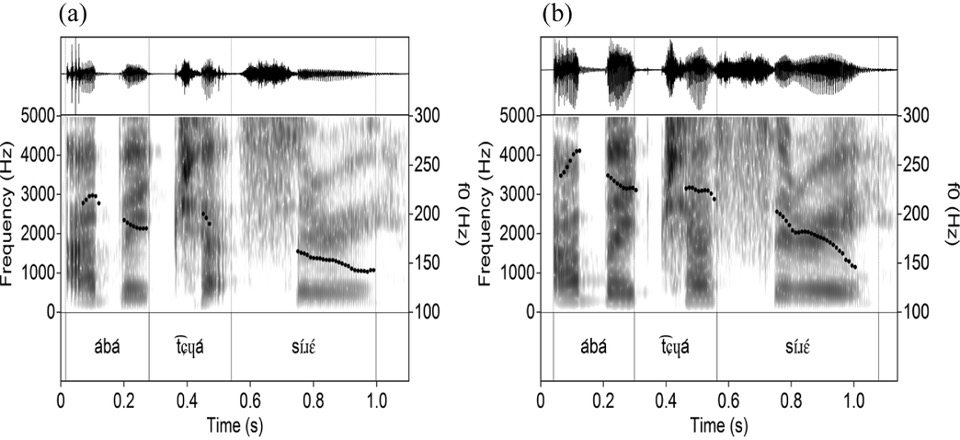
\includegraphics[width = 1\textwidth]{figures/akan.jpg}
	\caption{Waveforms and pitch curves of a declarative (right) and an interrogative by a female Akan speaker (Figure~7 in \textcite{genzel2020akan}) }\label{fig:akan}
\end{center}
\end{figure}

As shown in Figure~\ref{fig:akan}, the interrogative sentence is produced with a breathy voice quality at the end, as compared to the declarative sentence (F0 lowering here is a by-product of the laryngeal setting of producing the breathy voice). Table~\ref{tab:prosody:typology} lists some of the prosodic features that languages use to mark the differences between polar interrogatives and declaratives:



\begin{table}[H]
\begin{center}
\begin{tabular}{l|l}
\hline
Prosodic feature & Polar interrogative feature (language)\\
\hline \hline
Boundary tones: & H\% or LH\% (Dutch, French, Japanese) \\
 & HL\% (Roermond Dutch) \\
 & L\% (Catalan, Chickasaw, Bininj Gun-wok) \\
 \hline
Peak alignment & late peak alignment (Neapolitan Italian, Russian) \\
\hline
Peak height & Higher (Russian, Japanese) \\
\hline
Register expansion & Less downdrift (Wollof, Danish) \\
\hline
Final lengthening & Lengthening (Nateni) \\
\hline
Final voice quality & Breathy termination (Akan, Moba)\\
\hline
\end{tabular}
\end{center}
\label{tab:prosody:typology}
\caption{Intonational markings used to differentiate polar interrogatives and declaratives (adapted from \cite{butler2012typology})}

\end{table}%


Considering the fact that some languages do not use prosodic features for clause typing,\footnote{However, we do not have data on whether Vata or Shekgalagari uses prosody to distinguish imperatives from declaratives. Given the fact that languages tend not to have prosodic distinctions between declaratives and imperatives, our generalization has a good chance to hold.} it is possible that children do not have a priori knowledge that prosodic features are informative for clause type categorization. But what about speech acts? We do not have enough data from Vata to determine whether the question act could still carry a different set of prosodic features despite the fact that interrogatives are not marked by prosody, but given Gussenhoven and Chen's (\cite*{gussenhovenchen2000}) experiments with non-native prosodic contours, it is likely that speakers of Vata might be able to use rising intonation to identify questions. 

If children do not assume that prosody informs clause typing, Italian- and Portuguese-acquiring children might need to learn the connection between prosody and clause typing, in addition to learning clause type and speech act categories. But it is also possible that children do not need to learn this connection at all. If children assume that prosody informs speech acts, and that speech acts are informative of clause typing, prosodic information could indirectly help the learning of clause type categories. 

It is also possible that children come to the learning task assuming that prosody \tit{does} inform clause typing. For children learning languages like Vata, where prosody is irrelevant for clause typing in their language, the input might be such that this connection is simply uninformative. Thus, assuming a connection between clause typing and prosody would not make any difference for the learning the clause type categories. To test this possibility, we need to look at the input to Vata-acquiring children, and see if assuming the link between prosody and clause type would hinder children from learning the right clause type clustering. 

Another complication related to prosody is that languages use different prosodic features for clause typing, and many of them are not correlated with a rising F0 at the end. For example, Akan's breathy termination in fact results in the lowering of F0. Therefore, instead of having a built-in knowledge of the form ``final rise $\sim$ questionhood," children might need to learn which prosodic features are associated with which speech act/clause type clusters, the same way that they need to learn which morpho-syntactic features go with which clause type cluster.

Both English and Mandarin have dedicated morpho-syntactic features for interrogatives (e.g. subject-auxiliary inversion in English). But in both languages, it seems that there are also prosodic differences associated with interrogatives. We will discuss the prosodic features of these two languages in more details in Chapter~\ref{chap:man-cl} and Chapter~\ref{chap:prosody}.

\section{Acquisition of speech acts and clause types}
\label{sec:bg:acq}
\subsection{Early communicative abilities}
\label{sec:bg:acq:pre}
As mentioned in the previous chapter, it would be very useful for learners if they could rely on speech act information to learn how clause types are expressed in their language. Speech acts are, unfortunately, not directly observable, but there may be cues accessible to learners that are broadly indicative of speech act. One good candidate are cues for communicative intent.
Previous studies have shown that infants are sensitive to %can recognize
communicative intentions even in their first months of life, and they can distinguish signals for communication, such as eye contact, intentional pointing, and speech, from non-communicative signals. Infants tend to follow the gaze of their interactive partner. Newborn babies already show rudimentary form of gaze following (\cite{farroni2004gaze}); as young as 3 months of age, infants seem to automatically orient to gaze cues, as they could shift gaze fast with adult’s gaze direction (\cite{hood1998gaze}); 6-month-olds follow gazes that are communicative, such as adults' directly gazing at an object (\cite{gredeback2008gaze}), or being greeted (e.g. ``Hello!'') in infant-directed speech (\cite{senju2008gaze}). Human infants, but not chimpanzees, understand pointing as intentional (\cite{pika2006point, povinelli1997point,morissette1995joint}); 9-month-olds remember different aspect about an object depending on whether the object is presented in a communicative (such as pointing) vs.\ non-communicative scenario (\cite{yoon2008intent}); 12-month-olds not only follow the direction of pointing, but also infer that the pointing is to indicate information such as where a toy is hidden in hide-and-seek games (\cite{behne2005hide,behne2012point}). Starting from six months old, infants can readily interpret speech, but not other vocalizations like coughing, as indicating communicative intentions (\cite{vouloumanos2014intent}).

Of course, merely recognizing an act \emph{as communicative} is not the same as distinguishing speech acts -- beyond the recognition that there is communication, one needs to infer the function of the communication to approach speech act recognition.
Indeed, besides recognizing a signal as communicative, infants can attribute simple goals and desires to an agent, and use shared experience to infer their goals. By 9 months old, infants can recognize an agent's goal of reaching for an object (\cite{woodward1998goal,baldwin2001goal});\footnote{But studies show that still have difficulty with the avoidance type of goals until 14 months old (\cite{feiman2015goals}).} 14-month-olds can distinguish actions that are intentional and ones that are accidental, and only imitate actions that are intentional (\cite{carpenter1998intent,sakkalou2013goal}), and if things go wrong, they offer to help achieve others' goals (\cite{warneken2007goalrecog}); they could use shared experience such as cleaning up toys to interpret an agent's pointing as putting away the pointed object away, and would not attribute this goal to an agent who don't have the shared experience (\cite{liebal2009goal}).

Relatedly, it seems that infants have some understanding of other people's desires and beliefs, attitudes that are frequently associated with the speech acts of assertions, questions, and requests. For example, 9-months-old can distinguish whether someone is unwilling or unable to hand them a toy (\cite{behne2005goal}); 12-month-olds can use eye gaze and positive affect to infer which object an agent is going to reach for (\cite{phillips2002gaze}), and by 18 months old, infants use positive affect alone to infer which object the agent prefers, even if the preference is different from their own (\cite{repacholi1997desire}). Around 12 months old, infants can use pointing not to merely direct others' attention, but to request others to share information (\cite{kovacs2014request}); 13-month-olds seek information to clarify ambiguous situations (\cite{vaish2011request}); by 18 months old, infants are shown to be able to attribute beliefs to other people (\cite{onishi2005tom,surian2007tom,song2008earlytom,song2008false, scott2009tom,perner2012earlytom}, see \cite{scott2017review} for a recent review). 18-month-olds could use common ground knowledge shared with an agent to infer whether the agent is requesting an action with an object (e.g. open the door with the key) or simply playing with the object (\cite{schulze2015indirect}).%16-mo use pointing to solicit informaiton (\cite{begus2012point}); 2-year-olds are shown to use what others know when requesting help (\cite{oneill1996knowledge}). 
 


Infants also have some understanding of the norms of conversations. For example, from early on, they understand that conversations take turns. Longitudinal studies with 3 to 5-month-olds show that the overlap between infants' vocalization and parents' speech gradually decrease (\cite{hilbrink2013turn3mo}), and the rhythm of their vocalization starts to mimic the structure of a conversation, as they wait for parents to finish their turn (\cite{hilbrink2013turn,hilbrink2015,casillas2016corpus}); they also use turn transition points (e.g. questions) to cast predictive eye gaze to the next speaker (\cite{casillas2017turn}).

 
 %\textcite{} finds that 
 
In sum, this body of work suggests that by 18 months old, the communicative abilities needed to acquire the distinctions between speech acts and map them to clause types are in place. In the next section, we will see that indeed by this age, infants seem to figured out the major speech acts and are able to link them to their canonical clause types.



\subsection{Early knowledge of clause types and speech acts} \label{sec:bg:acq:spcl}

Previous studies show that children seem to have knowledge about clause types and the associated speech acts (in particular interrogatives and questions) from as early as 18 months old. 

Using corpus data, many studies show that infants can use one- and two-word utterances to express a variety of intentions that can be interpreted as \aqrs{} (\cite{bateson1975,bates1976language,ninio1994} among others); English-speaking children start producing interrogatives around 20 months starting with \twh-interrogatives (\citealt{tyack1977, stromswold1995, rowland2003cdswh}). From the comprehension side, results from corpus studies on parent-child interactions show that children begin to respond to parents’ questions, especially \tit{who, what, where} questions, appropriately around one and a half years old (\citealt{ervintripp1978, steffensen1978, shatz1978comprehension, shatz1978communicative, berningergarvey1981, shatzmccloskey1984, clark2015turn, moradlou2020} among others). 





Results from experimental studies show that around 12 months, English-speaking infants show sensitivity to differences in word order (\citealt{geffenmintz2015wordorder}) associated with declaratives and polar interrogatives. Data from preferential looking tasks show that already at 15 months old, infants look at the objects corresponding to the answers of \twh-interrogatives (\citealt{seidl2003wh, gagliardi2016wh, perkins2020filler}), though their success might not necessarily reflect knowledge of the syntax of \twh-interrogatives, as they might be relying on their knowledge of verb argument structure in the task (\citealt{perkins2019}). 

By 18 months old, infants seem to be able to distinguish questions from assertions, and use this distinction to infer the epistemic state of the speaker. \textcite{luchkina2018infant} test how well 18-month-olds’ learn labels of novel objects from speakers who made statements about familiar objects (e.g., \tit{This is a star}) and from speakers who asked questions (e.g., \tit{Is this a star?}). During the test phase, both types of speakers use statements to label a novel objects (\tit{Look, a lif! Lif!}). After repeating the statements several times, children are asked by an unfamiliar novel voice to look at one of the objects (e.g. \tit{Look, a lif! Where's the lif?}). They find that 18-month-olds only learn labels of objects from the speaker who made statements during the familiarization phase, but not from the question-askers. This result suggests that 18-month-olds can differentiate questions from statements, and furthermore, they can use this distinction to infer that question-askers might be a less reliable information source than statement-makers. 

\textcite{marshmallowqueen} demonstrate that 18-month-olds can associate interrogative syntax with the speech act of questioning with the preferential looking paradigm. In the experiment, infants watch a video of two puppets cheering a mechanical arm for delivering cookies into a box. During the test phase, one of the puppets leaves the scene while the cookie is being delivered, and is thus ignorant of whether there is a cookie in the box. Then participants either hear a polar interrogative \tit{is there a cookie in the box?} or a declarative \tit{there's a cookie in the box!} that could be uttered by either puppet. They find that at 18 months old, infants look more at the ignorant puppet when hearing the polar interrogative, suggesting that they understand the polar interrogative as a question uttered by the ignorant puppet.

\textcite{casillas2017turn} tap into children's knowledge of turn-taking to see if children differentiate questions from other types of speech acts. They measure how often children switch their gaze to track the upcoming speaker. Since questions are turn-transitioning points where a switch in speaker is mostly likely to happen, if children can identify questions, they should switch gazes to the upcoming speaker more often after questions. In the experiment, children are shown videos of a conversation between two puppets in one of four conditions: with normal speech, with words only (filtering out prosodic cues), with prosody, or with no speech. They find that even at 1 years old, children are faster at switching their gaze to the addressee after questions than non-questions in general. Breaking down the different cues to questions, they find that in the word-only condition, even 1-year-olds switch their gaze to the upcoming speaker more often after questions, but in the prosody-only condition, 5-year-olds still are at chance distinguishing questions from non-quesitons. These results suggest that 1-year-olds might be able to use the morpho-syntactic properties of interrogatives to infer questions. Similar results are replicated with 2.5-year-olds by \textcite{lammertink2015turn}.


As for imperatives and commands, \textcite{shipley1969} show that even in the ``telegraphic speech'' phase (15-30 months old), children respond appropriately to imperatives as commands. \textcite{orfitellihyams2012subj} show that 3-year-olds (and some 2.6-year-olds) can use the presence/absence of verb morphology to tell whether the sentence is a pro-drop declarative or an imperative, but it's possible that children in the experiments are using \tit{please} as a cue for command interpretation. 

Previous studies on questions in speech to children suggest that parents use questions in many different ways (\citealt{holzman1972, shatz1979, tamir1980, yu2019pedagogical}). In particular, compared to questions in adult-directed speech (\citealt{stivers2010}), parents tend to use question as a pedagogical strategy. \citealt{zaitsu2020} investigates the frequencies of the three basic clause types and the corresponding speech acts in speech to children between the age 1 to 3 from the Providence corpus (\citealt{ProvidenceCorpus}) of CHILDES (\citealt{CHILDES}). They find that although the three clause types generally are associated with their canonical speech acts, there are cases of mismatches (indirect speech acts). However these mismatches are often marked, and tend to form a systematic subcategory. For examples, when interrogatives are used as requests, we often see the presence of modals and attitude verbs in the sentence; when declaratives are used to perform questions, we often see rising prosody\footnote{Although they did not explicitly annotate the prosodic information; rising prosody is inferred from the use of question marks in the transcript.}. This is relevant because these systematic marking might alert the learners that these uses of the clause types may be somehow special. In particular, questions are often asked via rising declaratives, and requests made with interrogatives. 



Going beyond English and turning to Mandarin, we have less evidence for children's early knowledge of speech acts and clause types. Most study with younger children are documentations of their production data. Particularly, Mandarin-speaking children are observed to produce \ma-interrogatives, A-not-A interrogatives, and \twh-interrogatives before they turn 2 years old (\citealt{miao1986acq, miao1992, lee1989acq, litang1991int, lichen1997compprod, lichen1997comp, fan2012, lijingwong2017}). 

On the comprehension side, experimental studies testing children’s comprehension suggest that 18-30 month-olds can correctly link \twh-interrogatives to the question speech act, but are less likely to respond to A-not-A polar interrogatives (\textcite{moradlou2020}). However, this result might be due to the way the experiment is set up. During the experiment, children are asked polar interrogatives (e.g. \tit{Is this a duck?}) or \twh-interrogatives (e.g. \tit{What does a duck say?}) while looking at pictures of animals. But in this setting, particularly if the questioner is a person with authority, children might consider the polar question as redundant, and therefore tend to not respond to these questions. 

By 3 years old, Mandarin-children have adult-like interpretation of \twh-interrogatives (\citealt{fahn2003acq}), and that they can use prosodic information to determine whether the sentence is a \twh-interrogative or a declarative (\cite{WHanything}). In Mandarin sentences like  (\ref{bg-acq:negwh}) is ambiguous between a declarative and a \twh-interrogative. 

\bex{bg-acq:negwh}
\gll Xiaoyang mei	fang	\tun{shenme} shuiguo zai	xiangzili\\
Lamb \Neg{}	put	what		fruit		in	box\\
\trans a. ``What fruit didn't Lamb put in the box?''\\
b.	``Lamb didn't put any fruits in the box.''
\eex
In this case, the two interpretations are disambiguated by prosodic cues: assigning prosodic prominence on \tit{shenme} gives rise to a \twh-interrogative interpretation, and without prosodic prominence, the sentence is a declarative. \textcite{WHanything} show that 3-year-olds, like adults, can access both interpretations of the sentence.

\section{Summary}

In this chapter, I reviewed what we already know from the existing literature on the formal properties of clause types and speech acts and their analyses in the formal literature. Regardless of the theoretical approach, people agree on the three major clause types and their corresponding three major speech acts. 


Additionally, I reviewed literature on children's understanding of clause types and speech acts, and the linguistic and pragmatic capacities that they can draw from early in development, and what we know about the kinds of speech acts and clause types children are exposed to. The results from these studies suggest that by 18 months old, infants seem to have figured out the major clause types and speech acts, and the link in-between. These studies give us a developmental window for modeling the learning of clause types, namely that we need to take into account what infants know around 18 months old, to simulate how they figured out clause types and speech acts at this age. In the next chapter, I delve into the problem of how 18-month-olds figure out clause types. 





%In summary, children might face many challenges when learning interrogatives and their mapping to questions: English-speaking children should identify word order as a cue for interrogativity, but this information might be buried under many exceptions; Mandarin-speaking children should identify the markers for interrogativity (e.g.~\twh{}) despite some of these markers occurring in non-interrogative environments. Moreover, in both languages, children have to recognize the link between interrogativity and questionhood, which might be masked by exceptions in their input. So, how do children acquire interrogatives and their relationship to questions? In the next section, we will see that despite the noisiness of the input data, there is evidence suggesting that children nevertheless have adult-like understanding of interrogatives, questions, and their relationship at around three years old if not younger. 



 %\cite{evans2014ids} \cite{bernicot1987imp}


\chapter{Learning to identify clause types in English}
\label{chap:eng-cl}


As discussed in the previous chapters, cross-linguistically we see three major clause types, declaratives, interrogatives, and imperatives, corresponding to three main speech acts, assertions, questions, and commands/requests. We also saw in Chapter~\ref{chap:background} that by 18 months old, infants seem to have figured out the differences among these clauses and how they are associated with their canonical functions.  To gain this ability, they must have solved a number of learning problems. Specifically, as discussed in Chapter~\ref{chap:introduction}, learners need to solve the \tbf{clustering problem}, i.e. clustering clauses in the right three categories, and the \tbf{labeling problem}, i.e. linking each category to its function. 

%Given that infants's early success at identifying clause types,
This chapter investigates how learners solve these problems, especially the clustering problem, by probing the extent to which children need to rely on pragmatic information (i.e., inferring what speech act a given utterance of sentence is conveying). As discussed in Chapter~\ref{chap:introduction}, pragmatic information is essential for solving the labeling problem. The question I ask here, then, is whether pragmatic information is also crucial for solving the clustering problem as well. Will a learner strictly tracking formal regularities home in on the right three clusters of clauses? Will a learner privy to some speech act information fare better? How much pragmatic information is required? To answer these questions, I compare the performance of two computational models, a \gls{dlearnerabbr} and a \gls{plearnerabbr}. Since the success of the learning models should be commensurate with infants' early successes at identifying clause types, I will test the models using data from an annotated dataset I created with parental sentences in the Providence Corpus (\cite{ProvidenceCorpus}). One additional problem arises from our assumption that children have access to the speech act information, because we cannot rely on infants to perceive the pragmatic import of sentences in the absence of the knowledge of clause typing. While I will return to this problem in Chapter~\ref{chap:eng-sp}, in this chapter I ask how much pragmatics is needed for solving the cluster problem. To answer this question, I manipulated the ratio of noise in the pragmatic information and found that the clustering can succeed with very limited access to pragmatic information. . 

This rest of the chapter is organized as follows: 
In Section~\ref{sec:engcl:background}, I first briefly introduce the two computational models mentioned above, and how they can help us answer our questions (Section~\ref{sec:engcl:bg:learners}). I then review the formal features of English \diis{} (Section~\ref{sec:engcl:bg:grammar}), setting the stage for discussing the learning of these clause types. But these are features that English employs for clause typing, infants at 18 months old might not be able to perceive all of these features. To allow our models to best capture 18-month-olds' learning process, we need to look at 18-month-olds' linguistic capacity and knowledge with regard to these features. So in Section~\ref{sec:engcl:bg:assumptions} I briefly go through the linguistic capacities and knowledge of infants before 18 months old with regard to the formal features used for clause typing, which in turn will guide the way these features are coded in the corpus. 

In Section~\ref{sec:engcl:corpus}, I report results from a corpus study on parents' use of different clause types and speech acts, to give a quantitative description of the information present in the input. The annotated dataset that results from this corpus study will be used in our modeling experiments.

Section~\ref{sec:engcl:model} details the two computational models for the two learners, \gls{dlearnerabbr} and \gls{plearnerabbr}, to see if pragmatic information is needed for solving the clustering problem. I then manipulate the ratio of noise in the pragmatic information to see how much pragmatics is needed (Section~\ref{sec:engcl:model:noisy}). 

\section{Background}
\label{sec:engcl:background}

\subsection{Two learners} 
\label{sec:engcl:bg:learners}
As mentioned above, the question we set out to answer is whether morpho-syntactic features alone are sufficient for learners to solve the clustering problem. To this end, I build two computational models that learn the clustering of clauses, a \text{\distlearner{}} (\dlearnerabbr{}) and a \text{\praglearner{}} (\plearnerabbr{}). Both learners are forms of distributional learning: they track distributions of certain features in their input, and use these observations to infer the underlying categories that gives rise these distributions
(cf. \cite{feldman2013,gagliardi2017modeling,perkins2022vmodel,perkins2019,nguyenwilson2021}; see \cite{pearl2020review} for a recent review). Specifically, these two learners share the same goal of discovering the underlying clustering of sentences in parents' speech, i.e. to infer the abstract clause type categories in English. The difference between them lie in the sources of information they take as input. 

The \tbf{\distlearner{}} (\dlearnerabbr{}) assumes that learners track the statistical distributions of \tit{morpho-syntactic features} present in the surface forms of sentences to infer the abstract clause type category that gives rise to these distributions. This learner serves as our baseline; by looking at its performance, we will be able to see whether syntactic information by itself is sufficient for identifying clause types. 

The \tbf{\praglearner{}} (\plearnerabbr{}) also tracks the distributions of morpho-syntactic features, but at the same time, it keeps track of the speech acts expressed by these sentences as well. Thus, it infers clause type categories with information from both syntax and pragmatics. 

Thus, we would be able to answer the question of whether pragmatics is crucial for the clustering problem by comparing the performance of these two learners: if pragmatic information indeed helps the learner, not only with labeling but also with clustering, we would see \plearnerabbr{} outperforms \dlearnerabbr. Additionally, if \plearnerabbr{} indeed performs better, we can manipulate the ratio of noise in the pragmatic information that \plearnerabbr{} receives, to see how much pragmatic is needed for learners to solve the clustering problem. 


The success of these two learners depend on the specific features we feed into the models. In Chapter~\ref{chap:background}, we reviewed different taxonomies for speech act information and we may abstract away from language-specific ways of indicating force by having the \plearnerabbr{} keep track of pragmatic information in terms of knowing whether a sentence is an assertion, question or request. But the morpho-syntactic features for clause typing differ from language to language and to test whether the \dlearnerabbr{} can acquire clause typing from morphosyntax alone, we must test it on the actual features of the language we test it on. So, in the next section, we will go through the specific morpho-syntactic features that English employs for clause typing, to set the stage for our discussion of the learning of clause types. 


\subsection{Clause types in English} \label{sec:engcl:bg:grammar}

Generally, clauses in English are marked by the presence of verbs (\ref{ex:engcl:fragments}a). Sentences without verbs are often classified as fragments (\cite{sz1985speechact}), as in (\ref{ex:engcl:fragments}b):
\bex{ex:engcl:fragments}
\bxl{}
Mary hugged Ann.
\ex
Mary!
\exl
\eex

In this section, we will go over the properties of the three major types of clauses, \diis{}, in English. 
It is generally assumed that the declarative is the default clause type in English, and thus has the formal features [-int, -imp]. The hallmark of the [+int] value of English $C$ is subject-auxiliary inversion, which can be seen in polar interrogatives like  (\ref{ex:engcl:subjaux}a) and \twh-interrogatives like (\ref{ex:engcl:subjaux}b). 

\bex{ex:engcl:subjaux}
\bxl{}
Can Mary hug Ann?\hfill polar interrogative
\ex
Who can Mary hug? \hfill \twh-
interrogative
\exl
\eex


However, this association of word order and interrogativity has many exceptions. For example, in subject \twh-interrogative sentences like (\ref{ex:engcl:int-exceptions}a) and sentences with embedded interrogatives (\ref{ex:engcl:int-exceptions}b-c), the interrogative takes the same word order as a declarative. 

\bex{ex:engcl:int-exceptions}
\bxl{}
Who can hug Ann? \hfill subject \twh-interrogative
\ex
Mary wonders \tun{who Ann can hug.} \hfill embedded \twh-interrogative
\ex 
Mary wonders \tun{whether Ann can hug Sue.} \hfill embedded polar interrogative
\exl
\eex

As discussed in Chapter~\ref{chap:introduction}, these cases might be a problem for learners, as they obscure the mapping between the subject-auxiliary inversion rule and [+int]. While the presence of \twh-phrases in (\ref{ex:engcl:int-exceptions}a-b), and the complementizer \tit{whether} (\ref{ex:engcl:int-exceptions}c) in these sentences are also cues for [+int], these features suffer from a similar problem. For example, free relative sentences like (\ref{ex:engcl:whexceptions}) also appears with a clause-initial \twh-phrase, but the $C$ head this \twh-clause has the feature [-int] (\cite{bresnan1978free, caponigro2003free}):

\bex{ex:engcl:whexceptions}
Mary ate \tun{what Ann cooked.} \hfill Free relative sentences
\eex

%Mary claims that she ate what?
%in-situ \twh-questions,\footnote{We adopt the analysis given by \textcite{bobaljik2015echo} here that this type of \twh-questions are in fact declaratives with [-int] in their $C$. One of the reasons for this analysis is that these types of clauses cannot be selected by rogative verbs like \tit{wonder}:
%\begin{xlisti}
%\exi{(i)} *I wonders I should put this stuff where. \hfill (ex. (8b), \cite[p.18]{bobaljik2015echo})
%\end{xlisti}
%}

At the same time, some declaratives exhibit subject-auxiliary inversion as well, such as Negative Inversion sentences like (\ref{ex:engcl:neginvert}): these sentence are generally considered declaratives, but the auxiliary \tit{would} precedes the subjects in both.

\bex{ex:engcl:neginvert}
\bxl{}
Never in her life would Mary eat tripe.
\ex
Under no condition would Mary eat tripe.
\exl
\eex

These are cases where the speech act information might be particularly useful to a learner, as identifying the utterance as making an assertion would help the learner to avoid making the generalization that [-int] also triggers subject-auxiliary inversion. 

Imperatives (sometimes analyzed as $C$ having the feature [imp], \cite{platzack1997imp}) in English typically use a bare verb stem. In most cases, subjects are missing (\ref{ex:engcl:imp}a), but sometimes there are subjects expressing the addressee (\ref{ex:engcl:imp}b).

\bex{ex:engcl:imp}
\bxl{}
Be quiet!
\ex You be quiet!
\exl
\eex


In sum, declaratives ([$-$int, $-$imp] feature in $C$) in English are the unmarked clause type; interrogatives ([+int] in $C$) are associated with subject-auxiliary inversion, the presence of clause-initial \twh-phrases, and the presence of the complementizer \tit{whether}; imperatives ([+imp] in $C$) are marked by using verb stems, and by the absence of sentential subjects or having second person pronouns as subjects. So, to successfully infer the clause type categories, learners have to pay attention to morpho-syntactic features that include the presence or absence of the sentential subject, the form of the verb, the position of the auxiliary, the presence or absence of \twh-phrases in clause-initial position, and the choice of complementizers in the surface form of sentences. Table~\ref{tab:engcl:grammar} summaries the morpho-syntactic features and their associated clause types:


\begin{table}[H]
    \centering
\begin{tabular}{l|l } 
\hline
Feature  & Examples\\ 
\hline \hline
\multirow{2}{*}{$\pm$ \tsc{verb} }&
($+$) \tbf{Find} Elmo! \hfill Clause\\

&($-$) Elmo! \hfill Fragment
\\ 
\hline
\multirow{2}{*}{\tsc{$\pm$ subject} }&
($+$) \tbf{I}'ll take it. \hfill [$-$imp]\\

&($-$) Take it. \hfill [+imp]
\\
\hline
\multirow{2}{*}{\tsc{$\pm$ verb suffix} }&
($+$) Nobody feel\tbf{s} good huh? \hfill [$-$imp] \\

&($-$) Find Elmo! \hfill [+imp]
\\ 
\hline
\multirow{2}{*}{\tsc{$\pm$ subj-aux inversion} } & 
($+$) \tbf{Can you} find the ladybug? \hfill [+int]\\

&($-$) I can take it. \hfill [$-$int]
\\ 
\hline
\multirow{2}{*}{\tsc{$\pm$ sentence-initial \twh{} }} & 
($+$) \tbf{What} did you find? \hfill [+int]\\

&($-$) I found it. \hfill [$-$int] \\
\hline
\multirow{2}{*}{\tsc{complementizer} } & 
($+$) I know \tbf{whether} it's wrong. \hfill [+int]\\

&($-$) I know that it's wrong.\hfill [$-$int]
\\
\hline
\end{tabular}

\caption{Morph-syntactic features and their associated clause types}
\label{tab:engcl:grammar}

\end{table}

Of course, as we have discussed, many features do not have a one-to-one mapping with the abstract clause type categories. So apart from using the right features to cluster clauses, learners also need to avoid making certain generalizations about a feature in some cases (e.g. avoid associating subject-auxiliary inversion with declaratives upon seeing Negative Inversion sentences).  
 
While these features are significant in the grammar, it's likely that not all of these features (or the full-fledged version of these features) can be perceived by 18-month-olds. If we want to model how 18-month-olds learn clause types, the way we code these formal features in our corpus (which serves as the input to our models) has to be sensitive to their linguistic knowledge, and what they are able to perceive at the relevant age. In the next section, I will review what linguistic knowledge and capacities children have around 18 months with regard to these formal features. 

\subsection{Linguistic knowledge and capacities of 18-month-olds}
\label{sec:engcl:bg:assumptions}

Generally, infants have been shown to track distributional properties of various kinds, and 18-month-olds can perceive many grammatical features. How much do they know about the ones that are associated with English \diis{} (Table~\ref{tab:engcl:grammar})? In this section, I'll briefly review 18-months-olds' capability regarding the features reviewed in the last section, and along the way explain how we code these features in our corpus. % These features are included to give the \distlearner{} the best chance of succeeding. 

\tsc{$\pm$ Verbs:} By 18 months, infants can recognize whether there is a verb in a sentence. They can use the frequent frames (e.g. adjacency to function words like auxiliaries, pronouns, or have affixes) associated with verbs to categorize a novel word as a verb (\cite{echols2004verb, mintz2006verb,peterson2006aux,soderstrom2007sv, lidzoritaomaki2012, shi2014functional, helidz2017verb} among many others), suggesting that they have knowledge of verbs, and frequent verb frames. 

\tsc{$\pm$ Verb suffixes:} Around this age, infants can recognize some morphological markings on the verb.  As early as 6 months old, English-learning infants seem to be able to segment \tit{-s, -ed, -ing} from a nonce verb (\cite{kimmegha2016morph}). 15-month-olds can segment English verbal suffix \tit{-ing} from a word, but do not do so with pseudo-suffixes (\cite{mintz2013segmentation}); 18-month-olds can distinguish well-formed auxiliary-affix dependencies (e.g. \tit{is ...-ing}) vs. an ill-formed ones (e.g. \tit{can ...-ing}, \cite{santelmann1998morph}). Thus, we can assume that 18-month-olds can tell whether verb suffixes are present in a sentence.

\tsc{$\pm$ Subject:} Some studies have shown that infants have some knowledge about subjecthood by 18 months old. They show sensitivity to subject-verb agreement in English, as they prefer grammatical sentences over ungrammatical sentences with agreement violation (\cite{soderstrom2002agr, soderstrom2007sv, nazzi2011} among others), even if the subject is not immediately adjacent to the verb. They can also use the frame [subject pronoun + verb] to categorize novel words as verbs (\cite{babineau202014func,peterson2006aux, mintz2006verb,shi2014functional} among others). Moreover, and perhaps more importantly for our study, 12-month-olds are sensitive to the change in word order when the position of the subject and auxiliary is switched (\cite{geffenmintz2015wordorder}). While we do not have evidence that 18-month-olds can use the presence/absence of subjects to tell whether a sentence is imperative or not, we can assume that they can detect whether the subject is present or not.  % \footnote{\textcite{orfitellihyams2012subj} test whether 2.6-year-olds treat pro-drop declaratives and imperatives the same way, but it seems that the younger children do not )}


\tsc{$\pm$ Subj-aux inversion:} By 18 months, infants can recognize whether there is an auxiliary in the sentence, and are sensitive to the relative word order between the auxiliary and the sentential subject. As mentioned above, well before they turn 18 months old, infants can already use preceding auxiliaries to categorize a novel word into the verb category (e.g. \cite{peterson2006aux, mintz2006verb}), suggesting that they understand the relation between auxiliaries and verbs. Additionally, as mentioned above, 12-month-olds can already detect subject-auxiliary inversion (\cite{geffenmintz2015wordorder}, cf. \cite{erreich1984,ambridge2006auxinvert}); with both word order and prosodic cues, even 7-month-olds are able to detect the difference between polar interrogatives and declaratives (\cite{geffenmintz2011}). We therefore assume that infants are able to detect whether there is an auxiliary in the sentence, and further that they are able to detect whether the subject is preceding or following the auxiliary.

\tsc{$\pm$ Sentence-initial \twh{}:} \textcite{perkinslidz2021wh} shows that 18-month-olds, but not younger infants, begin to represent the sentence-initial \tit{which NP} as the head of a long-distance dependency. These results are suggestive, but we do not yet have evidence for the full range of \twh-phrases. In order to be conservative, we do not assume that infants have full-fledged knowledge of \twh{}. However, infants at this age have been shown to have the ability to tease apart functional from content words based on their acoustic and phonological properties (\cite{shi1999func,shi2014functional}) and it is reasonable to assume that they treat \twh{s} as functional items (\cite{perkins2019}). Therefore, we will consider \twh{} to be unknown to 18-month-olds, but still treat them as unknown \emph{functional} items (UFI), following \textcite{perkins2019}.\footnote{Note that \textcite{perkins2019} models what happens before 18 months, as her experiment narrows down the developmental window to 18 months old. Moreover, while her experiment only tests \tit{which}, there are some studies suggesting that 18-month-olds can also understand \tit{what}, \tit{who}, and \tit{where}. Thus, assuming that all \twh-items are unknown functional items might in fact be too conservative. In the future, I plan to see if loosening this assumption (e.g. assume that some \twh-items are known) will boost the performance of the \dlearnerabbr{}.} We can also assume that 18-month-olds can keep track of the position of these UFIs in a sentence, so we can code \twh-items as sentence-initial UFIs.\footnote{Other functional items for which we lack evidence for 18-month-olds knowing them include quantifiers, focus particles, complementizers (e.g. \tit{whether}), and certain conjuntors such as \tit{because}. I assume that these are UFIs as well.} 

\tsc{Complementizer:} Complementizers indicate the clause type of the embedded clause instead of the matrix clause. For simplicity, this dissertation mainly focuses on the matrix clause, and therefore this feature might not be relevant.  %So far, we do not have evidence for infants' knowledge of complementizers at this age, but, like \twh{s}, they might be able to categorize complementizers as functional items. We will treat these as UFIs. However, one thing to note is that complementizers indicate the clause type of embedded clauses, but for simplification, this dissertation mainly deals with matrix clauses. Nonetheless, having  %So we will treat these as UFIs as well. Since infants can identify verbs, we assume that they can track that certain UFIs occur post-verbally. 


%Table~\ref{} summarises our assumptions about 18-month-olds' knowledge of the set of formal features that associated with clause typing.


%Finally, infants can perceive some features of prosody, and might be able to use some non-clause type-related features to infer speech acts. We will come back to both in Chapter~\ref{chap:eng-sp}.

In summary, apart from clause-initial \twh-phrases and complementizers (which we will assume to be perceived as clause-initial UFIs), 18-month-olds have the formal features relevant for clause typing in English. But how do parents use clause types and speech acts? How serious is the many-to-many mapping problem, both for the mapping between clause type and speech act, and for the mapping between formal features and clause type? We will address these questions with a corpus study. %The annotated dataset resulted from this study will be used in our computational modeling experiments.

\section{Corpus study}
\label{sec:engcl:corpus}
To understand how infants figure out clause types and speech acts, we not only need to know which features they can in principle understand, but also need to establish what kind of information is even \emph{available} to them in the input. In this section, I’ll report findings from the corpus study on parental input to English-speaking infants. 


\subsection{Corpus and methods}
\label{sec:engcl:corpus:methods}
%%%%PAST TENSE
For this study, we used data from the Providence sub-corpora (\cite{ProvidenceCorpus}) from CHILDES (\cite{CHILDES}), which consists of parent-child interactions from 6 families recorded between 2002-2005 in Providence, RI. We selected this particular corpus because it covers children’s interaction with parents at the critical age that we are interested in ($\leq$ 18 months old). Additionally, it contains transcripts, audio, and video data, providing us with an opportunity to not only look at the morpho-syntax of parents’ sentences, but also their prosodic information, and even parents’ behavior accompanying each utterance. Parent-child interaction data from five typically developing children in this corpus were included in this study: Alex, Lily, Naima, Violet, and William. %For each session, we used the transcript to annotate  

We sampled 500 conversational turns from each session, and annotated the resulting dataset with the annotation schema detailed in the next section.\footnote{The full annotation schema can be accessed here: \url{https://github.com/Yu-an/annotation_tool/blob/main/schema.pdf}} For the clause type and speech act information, each annotator completed a subset of transcripts (20\% were double annotated, mean Cohen's $\kappa$ = 0.84, range 0.8-0.91, `almost perfect’ per Landis and Koch's (\cite*{landis1977iaa}) descriptive division). To annotate the speech act information, annotators were asked to look at 20 utterances before and 2 utterances after the current utterance in the conversation, as well as consulting the videos for contextual information. If the annotator could not decide on an annotation despite the contextual information, a second person would be consulted, and if still unclear, the utterance would be eliminated. For the morpho-syntactic features, initial annotation was generated by a script (\textcolor{red}{url}) using the morphological tagging provided by CHILDES, and then manually corrected. 

In total, 9147 utterances were annotated. We will return to the video and audio part of the annotation process in Chapter~\ref{chap:eng-sp}.




\subsection{Annotation schema}
\label{sec:engcl:corpus:schema}

\subsubsection{Clause Type}

All sentences in our sample were annotated with clause type information: declarative (\ref{ex:engcl:annt:cl:decl}), interrogative (\ref{ex:engcl:annt:cl:int}), or imperative (\ref{ex:engcl:annt:cl:imp}). Minor clause types like exclamatives were annotated as Other (\ref{ex:engcl:annt:cl:other}), as our primary interest is on the three major clause types (and we do not have evidence for 18-month-olds' understanding of minor clause types). Two other categories were also included: Fragments and Ambiguous cases. In cases where the utterance only contains a noun or an injective without verbs like (\ref{ex:engcl:annt:cl:frag}), the utterance was annotated as a Fragment: 

\bex{ex:engcl:annt:cl}	
Clause type
\bxl
\label{ex:engcl:annt:cl:decl}
It’s all twisted. \hfill Declarative
\ex \label{ex:engcl:annt:cl:int} What happened?	\hfill Interrogative
\ex \label{ex:engcl:annt:cl:imp} Throw it.\hfill Imperative
\ex \label{ex:engcl:annt:cl:other} What a nice day! \hfill Other
\ex \label{ex:engcl:annt:cl:frag}	Elmo!\hfill	Fragment
\ex \label{ex:engcl:annt:cl:amb} Wanna get down?	\hfill Ambiguous
\exl
\eex

Ambiguous cases are sentences that do not contain enough information to decide the clause type categories. For example, sentences like (\ref{ex:engcl:annt:cl:amb}) could either be a case of ellipsis from the declarative sentence \tit{you want to get down}, or ellipsis from the polar interrogative \tit{do you want to get down}. In both cases, there is no overt morphological marking on the verb \tit{want}, so after going through the ellipsis operation, the two sentences would end up with the same surface form. If the verb has an overt suffix, however, the two possibilities would give rise to different surface forms. For example,(\ref{ex:engcl:annt:disamb:dec}) has to be a case of left-edge ellipsis from polar interrogative \tit{are you coming}, and cannot be from a declarative sentence like \tit{you come}, as ellipsis the latter would not give us the \tit{-ing} morpheme on the verb. For the same reason, (\ref{ex:engcl:annt:disamb:int}) cannot be elided from polar interrogative \tit{Did you go to the store yesterday}. Thus, the two sentences in (\ref{ex:engcl:annt:disamb}) were annotated as interrogative and declarative respectively, but (\ref{ex:engcl:annt:cl:amb}) was annotated as Ambiguous.

\bex{ex:engcl:annt:disamb}
\bxl\label{ex:engcl:annt:disamb:dec} Coming? \\
\cmark \tit{Are you coming?}\\
\xmark \tit{You come?}
\ex \label{ex:engcl:annt:disamb:int} Went to the store yesterday? \\
\cmark \tit{You went to the store yesterday?}\\
\xmark \tit{Did you go to the store yesterday?}
\exl
\eex

Interrogatives were further divided into subcategories as polar (\ref{ex:engcl:annt:subI:pol}), \twh{} (\ref{ex:engcl:annt:subI:wh}), and disjunctive interrogatives (\ref{ex:engcl:annt:subI:disj}):

\bex{ex:engcl:annt:subI}	Sub-types of interrogatives
\bxl\label{ex:engcl:annt:subI:pol}
Is that a big bird shovel? \hfill	Polar interrogative
\ex\label{ex:engcl:annt:subI:wh}	Who is that?\hfill	\twh-interrogative
\ex\label{ex:engcl:annt:subI:disj}	Do you want water or juice? \hfill Disjunctive interrogative
\exl
\eex

\subsubsection{Speech Act}

Three major speech act categories, assertions, questions and requests/commands, were labeled;%\footnote{The distinction between requests and commands can be subtle, and often involves the calculation of the social hierarchy between conversational partners. As parents hold authority over the child, even if the parent intend an utterance to be a request, it could be perceived by the child as a command. Therefore, I did not make a distinction in this dissertation.}
minor speech act categories such as exclamations and greetings were labeled as Other:

\bex{ex:engcl:annt:sp}
\bxl\label{ex:engcl:annt:sp:a} It’s all twisted!\hfill	Assertion
\ex\label{ex:engcl:annt:sp:q} Is that the postman?\hfill		Question
\ex\label{ex:engcl:annt:sp:r} Throw it!	\hfill		Request/command
\ex \label{ex:engcl:annt:sp:o} Good morning! \hfill Other
\exl
\eex

As discussed in the last chapter, while the three major clause types are associated with the three major speech acts in most cases, there are some mismatching cases. For example, (\ref{ex:engcl:annt:indirect}) is a polar interrogative, but the non-literal (i.e. indirect speech act in Searle's (\cite*{searle1975indirect}) terminology) act of the utterance is to make a request.
%We labeled the non-literal (indirect) speech act (i.e. request) for these cases.
In such cases, we annotated the utterance with the non-literal (indirect) speech act, i.e.\ (\ref{ex:engcl:annt:indirect}) was annotated as a request.

\bex{ex:engcl:annt:indirect}
Can you put that down?
\eex 

Another complication comes from rising declaratives like (\ref{ex:engcl:annt:rd}). As discussed in the last chapter Section~\ref{sec:bg:theory:prosody}, there is a live debate on whether to label these cases as declaratives, interrogatives or some more sophisticated category (\cite{gunlogson2008,  farkasroelofsen2017}). 

\bex{ex:engcl:annt:rd}
is it raining $\nearrow$
\eex

We followed \textcite{gunlogson2008} in classifying the form of (\ref{ex:engcl:annt:rd}) as declarative, and labeled the speech act as either question or assertion depending on the contextual information, following \textcite{jeong2018, goodhue2021rd}. We will return to the complications brought on by prosody in Chapter~\ref{chap:eng-sp}.

\subsubsection{Formal features}

As reviewed in the last two sections, infants at 18 months old can perceive many morpho-syntactic cues related to clause typing, as recorded in Table~\ref{tab:engcl:grammar}. In particular, infants at this age can detect whether there is a verb in the sentence; whether the verb has suffixes; whether there is a subject in the sentence, and its position in the sentence (whether in canonical pre-verbal position or inverted with an auxiliary); and whether there is an auxiliary in the sentence. Infants might not be able to identify all the \twh-items or complementizers at this age, but they might be able to classify them as functional elements, as they may know the distinction between functional and content elements. We therefore put \twh-items, quantifiers, connectives (except for \tit{and}), and focus particles in one category ``unknown functional item (UFI),'' and annotated its position in a sentence: sentence initial, sentence-medial but before the verb, or after the verb. Each sentence was annotated with whether or not a specific cue is present. Table~\ref{tab:eng-cl:formal-schema} summarizes the features we annotated and their examples.  


\begin{table}[H]
    \centering
\begin{tabular}{r|l } 
\hline
& Examples\\ 
\hline \hline
\multirow{2}{*}{\textpm Verb} & 
($+$) \tbf{Find} Elmo! \\

&($-$) Elmo! 
\\ 
\hline
\multirow{2}{*}{\textpm Subject} & 
($+$) \tbf{I}'ll take it.\\
&($-$) Take it. \hfill
\\
\hline
\multirow{2}{*}{\textpm Verb Suffix} & 
($+$) Nobody feel\tbf{s} good huh?\\

&($-$) Find Elmo! 
\\ 
\hline
\multirow{2}{*}{\textpm Auxiliary} & 
($+$) \tbf{Can} you find it? \\

& ($-$) I found it! 
\\ 
\hline
\multirow{2}{*}{\textpm Subj-aux inversion} & 
($+$) \tbf{Can you} find the ladybug?\\ %\hfill \tcb{Interrogative}

&($-$) I can take it. %\hfill\tcr{Declarative}
\\ 
\hline
\multirow{2}{*}{\textpm Sentence-initial UFI}& 
($+$) \tbf{What} did you find?\\ %\hfill \tcb{Interrogative}

&($-$) I can take it.\\
\hline
\multirow{2}{*}{\textpm Pre-verbal UFI}&
($+$) Raccoon \tbf{only} comes out at night.\\

&($-$) I can take it.\\
\hline
\multirow{2}{*}{\textpm Post-verbal UFI} & 
($+$) I know \tbf{what}'s wrong.\\

&($-$ I know you can do it.
\\
\hline
\end{tabular}

\caption{Morpho-syntactic cues and their examples}
\label{tab:eng-cl:formal-schema}
\end{table}





\subsection{Results}
\label{sec:engcl:corpus:results}


\subsubsection{Overview}
With the schema given above, an annotated dataset consisting of 9047 utterances was created. As we are primarily interested in the form and function of parents' sentences in this chapter, we excluded children's utterances and uninterpretable utterances from the dataset. In total, 7039 utterances were analyzed.  Figure~\ref{fig:real-cldist} shows the distribution of clause types in the dataset. Declarative clauses are the most frequent clause type, followed by interrogatives and imperatives. 


\begin{figure}[H]
    \centering
    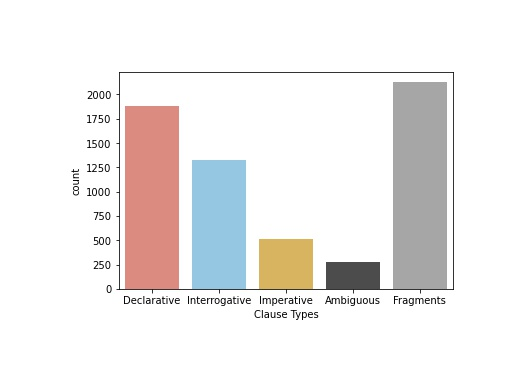
\includegraphics[width=0.7\textwidth]{figures/real-cldist.jpg}
    \caption{Distribution of clause types in the corpus}
    \label{fig:real-cldist}
\end{figure}

Zooming in on interrogatives, \twh-interrogatives are more frequent than polar interrogatives; only 2 cases of disjunctive interrogatives were found in the dataset. Figure~\ref{fig:real-subI} shows the distribution of the subcategories of interrogatives. 

\begin{figure}[H]
    \centering
    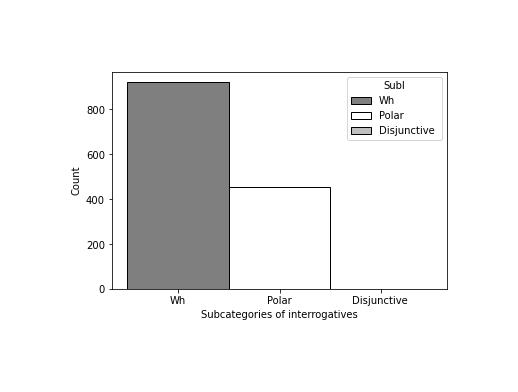
\includegraphics[width=0.7\textwidth]{figures/real-subI.jpg}
    \caption{Subcategories of interrogatives}
    \label{fig:real-subI}
\end{figure}

\begin{figure}[H]
    \centering
    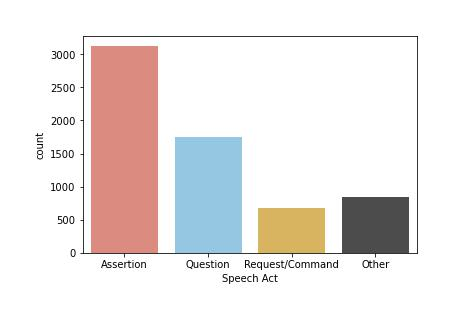
\includegraphics[width=0.7\textwidth]{figures/real-sp.jpg}
    \caption{Distribution of speech acts in the corpus}
    \label{fig:real-sp}
\end{figure}

As shown in Figure~\ref{fig:real-clsp} and \ref{fig:real-spcl}, the three major clause types are mostly used for their canonical functions. The majority of declaratives are used to express assertive force; the majority of interrogatives are used to express question force; and the majority of imperatives are used to express command/request force. 

\begin{figure}[H]
    \centering
    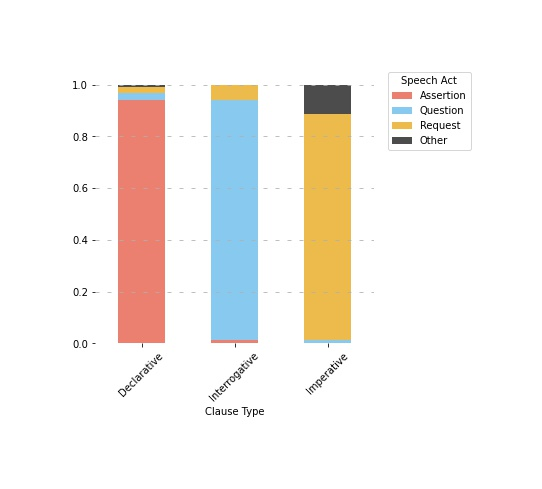
\includegraphics[width=0.7\textwidth]{figures/real-clsp.jpg}
    \caption{The speech acts performed by each clause type in parents' speech}
    \label{fig:real-clsp}
\end{figure}

Conversely, as shown in Figure~\ref{fig:real-spcl}, the majority of assertions are expressed by declaratives, the majority of questions by interrogatives, and the majority of commands/requests by imperatives.

\begin{figure}[H]
    \centering
    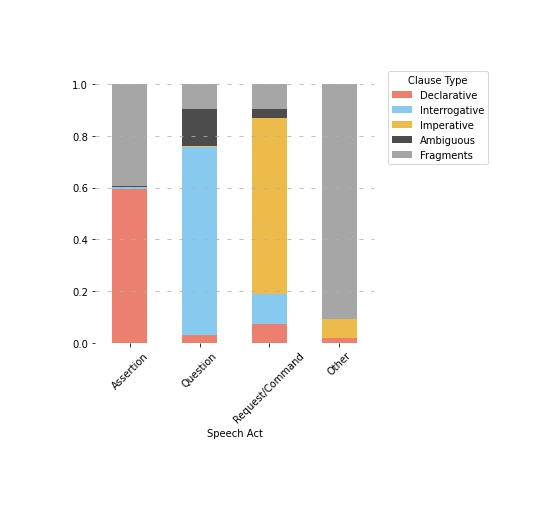
\includegraphics[width=0.7\textwidth]{figures/real-spcl.jpg}
    \caption{The clause type used to express each speech act in parents' speech}
    \label{fig:real-spcl}
\end{figure}


The few cases of mismatches between clause type and force appear to show that such mismatches are marked by certain morpho-syntactic features. For example, declarative and interrogative sentences used for requests/commands tend to have modals, attitude verbs, or future morphology in the sentence:

\bex{eng-cl:dec-req}
\bxl{}	I need you to help me.		\hfill	Mother of William, Session 010605
\ex	Can you say hi?				\hfill	Mother of Lily, Session: 010117
\ex	(previous utterance: I'm gonna do some work.)\\
And you’re gonna do some coloring.\hfill		Mother of Violet, Session: 010407
\ex  Are you gonna read to Mommy?	\hfill	Mother of Lily, Session 010102
\exl
\eex 

Declarative and imperative sentences used as questions are predominantly marked with final rise intonation. We will return to the prosodic features of each clause type in Chapter~\ref{chap:eng-sp}.

%, as in (\ref{eng-cl:dec-rise}a-b), or have embedded interrogatives (\ref{eng-cl:dec-rise}c):
\begin{comment}
\bex{eng-cl:dec-rise}
\bxl{}
Try this again?			\hfill Mother of William, Session 010605
\ex Oh , you don't wanna play with this ? \hfill	Mother of Naima, Session 001126
\ex Tell Mommy what it says. \hfill Mother of Alex, Session 010427 
\exl
\eex

\end{comment}

\begin{figure}[H]
    \centering
    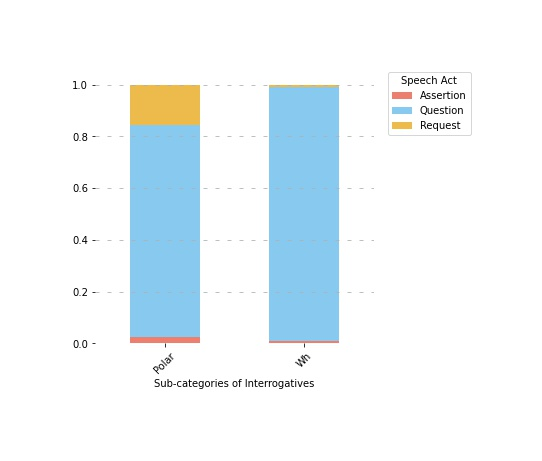
\includegraphics[width=0.7\textwidth]{figures/real-subIsp.jpg}
    \caption{The speech act expressed by different subcategories of interrogatives}
    \label{fig:real-subIsp}
\end{figure}




Turning now to the speech acts expressed by interrogatives, Figure~\ref{fig:real-subIsp} shows the proportion of speech acts that polar and \twh-interrogatives express. The only two examples of disjunctive interrogatives were used both as questions, and are thus not graphed in this figure. Polar interrogatives are used to express more types of speech acts than \twh-interrogatives: around 18\% of polar interrogatives were used for indirect requests like in (\ref{ex:engcl:int-req}) or assertions like in (\ref{ex:engcl:int-asst}):
\bex{ex:engcl:int-req}
Can you give Mommy the ball? \hfill Mother of William, Session: 010412
\eex
\bex{ex:engcl:int-asst}
Doesn’t he have sharp teeth?	\hfill	Mother of Lily, Session: 010611
\eex

Few \twh-interrogatives are used as non-question. We found 4 cases of \twh-interrogatives used to indirectly make a request (\ref{eng-cl:wh-req}), and indirectly making assertions by way of asking rhetorical questions (\ref{eng-cl:wh-asst}):\footnote{We did also find sentences with \tit{how about/what about} (Rawlins and Bledin~2021), but the majority of these sentences do not come with a verb and were considered fragments (\ref{eng-cl:howabout-frag}). But we also found one case of \tit{how about} interrogative with a verb (\ref{eng-cl:howabout-int}), and the primary intention of the utterance is to make a request. 

\begin{xlisti}
\ex \label{eng-cl:howabout-frag} How about this one?	\hfill	Mother of Alex Session 010512
\ex \label{eng-cl:howabout-int} How about we do these babies. \hfill	Mother of Lily, Session 010102
\end{xlisti}
}


\bex{eng-cl:wh-req}
Why don’t you turn around.	\hfill Mother of William, Session 010619
\eex
\bex{eng-cl:wh-asst}
\twh-interrogatives as assertions
\bxl{}
Who doesn’t love cheese?\hfill	Mother of Lily, Session: 010117
\ex Why are there no pens in this family?\hfill	Mother of Violet, Session: 010407
\exl
\eex


In sum, clause types are typically used for their canonical function in the input to children. This suggests that having speech act information could indeed be more helpful than hurtful for learning to categorize clauses into clause types.

\subsubsection{Morpho-syntactic cues}
\label{sec:engcl:corpus:formal}
We now turn to the formal cues of each clause type, as reviewed in Section~\ref{sec:engcl:bg:grammar}. In this analysis, we excluded fragment utterances that only contain a noun (\tit{Birdie!}) or an interjective (\tit{Oh}). In total, 3923 sentences were included in the analysis. The distribution of the morpho-syntactic cues listed in Table~\ref{tab:eng-cl:formal-schema} across different clause types is shown in Figure~\ref{fig:real-syncluster}. Darker colors represent the number of sentences with the morpho-syntactic property, and lighter colors represent sentences without the property.%The x-axis of the figure represents the counts of sentences, and the eight morpho-syntactic features are listed along the y-axis. Each graph is split in the middle: to the left of the line, bars with darker colors represent the counts of declarative, interrogative, or imperative sentences with this specific feature, and to the right, bars with lighter colors represents the number of sentences without this feature. 





\begin{figure}[H]
    \centering
    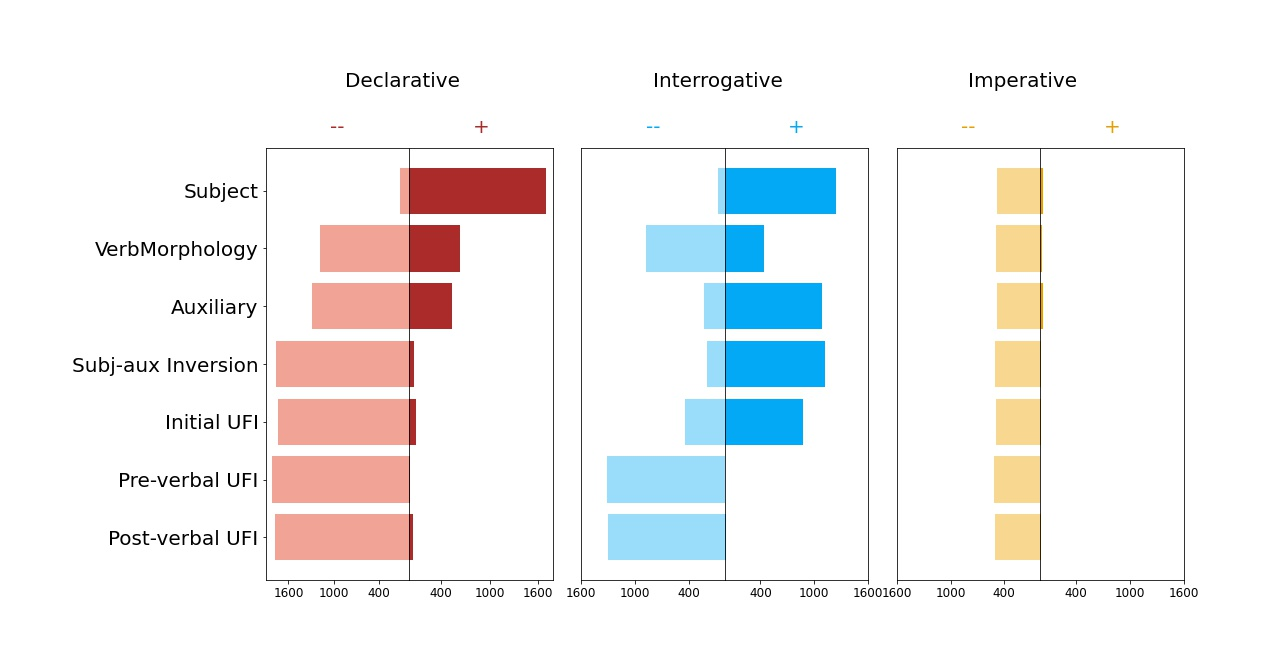
\includegraphics[width=1\textwidth]{figures/real-syncluster.jpg}
    \caption{Number of sentences with/without various formal cues in each clause type; darker colors represent number of sentences with the cue, lighter colors, number of sentences without the cue }
    \label{fig:real-syncluster}
\end{figure}

We can see that the three main clause types have different formal profiles in the input, but the general pattern aligns with the properties of [\textpm int] and [\textpm imp] discussed in Section~\ref{sec:engcl:bg:grammar}: interrogativity is associated with subject-auxiliary inversion and sentence-initial \twh{} (i.e. an unknown functional item for infants); [+imp] is associated with the lack of verb suffixes (i.e. the use of bare verb stems) and subjects; declaratives, the default clause type, are associated with the presence of subjects and verb suffixes, and the lack of subject-auxiliary inversion and clause-initial UFIs. 

From these results, we can see that the formal signatures of each clause type is consistently present in the input: auxiliary-inversion for interrogatives and the lack of subjects and verb suffixes for imperatives. But how informative are these cues to clause typing? And what can or does speech act information add to these cues? In the next section, I train two logistic regression models with actual clause type labels (i.e. using a supervised learning method in machine learning terms) to see how well the models find statistical regularities related to clause typing in the data. 

% However, we do see some features that might not matter for clause typing are also present, such as the presence of subjects in declaratives and interrogatives. 

\subsubsection{Informativeness of syntactic and pragmatic cues}
\label{sec:engcl:corpus:supervised}
In the previous section, we saw that in parents' speech to 18-month-olds, the three clause types are mostly mapped to their canonical functions, and that they have different morpho-syntactic profiles as expected. In this section, I evaluate the informativeness of syntactic and pragmatic cues by comparing two supervised learning models. Unlike the models simulating the \dlearnerabbr{} learner and the \plearnerabbr{} learner I will discuss later, these two supervised models were trained on a subset of our annotated dataset with clause type labels given as input. That is, the models are given correctly annotated data for training (hence the term ``supervised'') and attempt to determine the significant statistical regularities associated with each clause type. After the training phase, these models were tested on the part of data they have not seen, to see how well they could use the statistical regularities discovered in the training data to predict clause type labels. 

The supervised \dlearnerabbr{} learner uses morpho-syntactic cues as predictors for clause typing, while the supervised \plearnerabbr{} uses both morpho-syntactic and speech act information. Both are multinomial logistic regression models trained on 90\% of the annotated dataset, with clause type categories as dependent variable (declarative as the baseline), and a set of morpho-syntactic cues as predictors. As discussed in Section~\ref{sec:engcl:bg:grammar}, [+int] is associated with the presence of cues (e.g. auxiliary inversion, clause-initial \twh{}, complementizer), while [+imp] is associated with the absence of cues (e.g. verb suffix, subject). So the set of syntactic predictors in our models is [-subject, $-$verb suffix, +auxiliary, +subj-aux inversion, +clause-initial UFI,+pre-verbal UFI, +post-verbal UFI]. We then test the performance of both on the unseen 10\% of the data to see how well they predict the clause type categories. We calculated the rand score of both models to evaluate their performance. The rand score is normally used to measure the similarity between two data clusterings (\cite{rand1971}), calculated by taking all pairs of samples and counting ones that are assigned to the same or different clusters in the predicted and true clusterings:

\begin{equation} \mbox{RI} =\frac{ \mbox{number of agreeing pairs}}{ \mbox{number of pairs}} 
\end{equation}


The performance of the two models over 10 iterations is shown in Figure~\ref{fig:super-compare-rand}. Overall, the supervised \praglearner{} outperforms the supervised \distlearner{}, suggesting that the speech act information provides additional information for clause typing.


\begin{figure}[H]
    \centering
    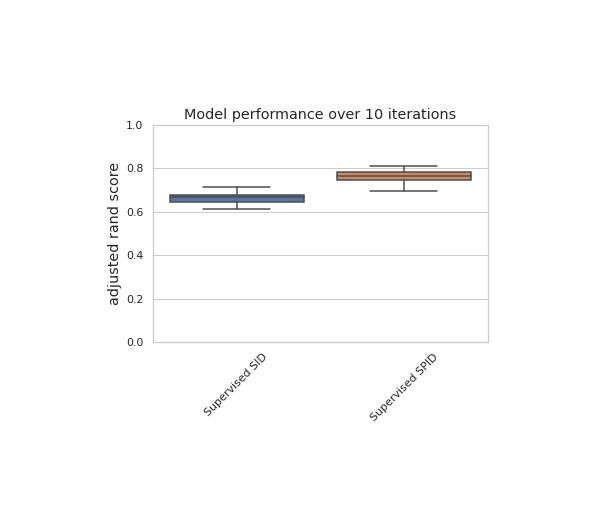
\includegraphics[width=0.6\textwidth]{figures/super-compare-rand-name.jpg}
    \caption{Comparing the two supervised models by rand score (performance over 10 iterations)}
    \label{fig:super-compare-rand}
\end{figure}


%Both models found the same morpho-syntactic regularities the coefficients the two models assigned to the morpho-syntactic predictors 

Our next question is how well the models know the morpho-syntactic makeup of each clause type. This can be inferred from the coefficients that the two models assign to the morpho-syntacitc predictors. A bigger coefficient assigned to a predictor means that the model assigns it a higher significance. As declarative clauses were used as the baseline, the coefficients should in particular be interpreted as indicating how much a specific morpho-syntactic cue contribute to the increase/decrease in the log odds of the sentence being classified as interrogative/imperative vs. declarative (i.e. if a sentence has a morpho-syntactic cue, how likely will it have the feature [+int] or [+imp] as opposed to the default clause type [-int, -imp]). For our purposes, significance was calculated using a two-tail $z$-test. Details of the models, coefficients, and $p$-values are reported in \mycode{}. %Appendix~\ref{appx:engcl}. 
Table~\ref{tab:engcl:corpus:formal} summarizes the morpho-syntactic profile of each clause type.

\begin{table}[H]
\begin{center}
\begin{tabular}{c|p{10cm}}
\hline
Clause Type Feature & Morpho-syntactic cues\\
\hline \hline
Interrogatives (+int) & +auxiliary, +subject-auxiliary inversion, +sentence-initial UFI\\
\hline
Imperatives (+imp) & $-$subject, $-$verb suffix\\
\hline \hline
\end{tabular}
\end{center}
\caption{Morpho-syntactic cues associated with interrogatives and imperatives compared to declaratives}
\label{tab:engcl:corpus:formal}
\end{table}%


As seen in the table, compared to declaratives, interrogatives are more likely to have subject-auxiliary inversions and sentence-initial UFIs; imperatives are more likely to have null subjects and bare verb stems, as expected. Some associations were less expected. For example, [+int] is associated with [+auxiliary], which is not predicted by our theory of clause typing in English. But this in fact reflects another formal property of English [+int], namely \tit{do}-support. Whenever T and V are not syntactically adjacent (either because T to C movement or negation in declaratives and imperatives), \tit{do} is inserted. Since T to C movement is common in interrogatives, but negation is less common in imperatives and declaratives, this elevates the rate of auxiliary in interrogatives relative to the other kinds of clauses. %Since \tit{do} is optional in declaratives and imperatives, but necessary in interrogatives, it is not surprising that auxiliaries appear more often in interrogatives. 

%A more realistic model for infant language learning would be unsupervised model where they discover the clustering of sentences. Nevertheless, the supervised learners are useful as an estimate of how informative formal and speech act features are for the task of inferring clause type.

Of course, these two models do not reflect how infants learn clause typing, as they were given clause type information. Infants must learn clause typing without having access to data of which the clause type label is given. These supervised models are nevertheless useful for appreciating the information contained in the data that children receive as input. They allow us to measure the correlation between the features and clause type categories, which provides an upper limit on how much information could be conveyed by the morpho-syntactic cues.. The results from these two models suggest that the information needed for clause typing is indeed available in the input and, in particular, from the categories with which we annotated our data. In the next section, we will get one step closer to addressing how infants learn clause types by removing the actual clause type labels from our models (switching to what in machine learning is known as ``unsupervised learning''). This makes the learning models more similar to the actual learning task where infants are not given these labels. Using these models, we can ask whether a learner that expects three clause type categories would be able to solve the clustering problem discussed in Chapter~\ref{chap:introduction} on the basis of morpho-syntactic cues alone. We then consider the question of whether adding in speech act information would help. Finally, as speech act information is likely not perceived veridically (e.g. due to developing pragmatic skills at this age), I ask how much pragmatics learners need to learn clause type categories. 


\section{Modeling the learning of clause types}
\label{sec:engcl:model}
Now that we have seen that the relevant information for clause typing is present in the input, our next step is to see whether a learner that can only perceive the morpho-syntactic cues would have enough information to find the right clause types. 

As discussed in Section~\ref{sec:engcl:bg:learners}, I examine the role of pragmatics computationally by building two Bayesian clustering models. The two models simulate a \distlearner{} and a \praglearner{}. Both are distributional learning models: as input, they observe the distribution of several morpho-syntactic cues that are identifiable by infants at 18 months old, and they use that information to cluster sentences into three clause type categories. Given that, cross-linguistically, the same three types of clause types (\diis{}) are associated with three major speech acts (\aqrs{}), it is reasonable to assume that an expectation for three clause types is innate. Even if learners do not have this innate expectation, determining whether learning can succeed with this expectation is a first step in determining whether it is possible to learn the clause types without it. Our learners thus assume that there are three categories, and only have to discover what these categories are, based on formal features. The \praglearner{} additionally observes speech act information and assumes that it is related to clause type. We further manipulated the ratio of noise in the pragmatic information that the pragmatically informed learner is given, to test how much pragmatics the learner needs.


This section is organized as follows. Section~\ref{sec:engcl:model:spec} specifies the generative models simulating the two learners. Then I specify how the two models infer clause type categories in Section~\ref{sec:engcl:model:infer}. Section~\ref{sec:engcl:model:results} reports the simulations with English infant-directed speech demonstrating that pragmatic information is crucial for finding the right clause type clustering, and that this pragmatic information does not have to be perfect, as even with 80\% of noise, it still boosts the performance of the \praglearner{}. 

\subsection{Generative models}
The two models simulating the \distlearner{} and the \praglearner{} are Bayesian clustering models, illustrated in Figure~\ref{fig:engcl:model}.% 

\label{sec:engcl:model:spec}

\begin{figure}[H]
\begin{minipage}[b]{0.45\linewidth}	
\begin{center}
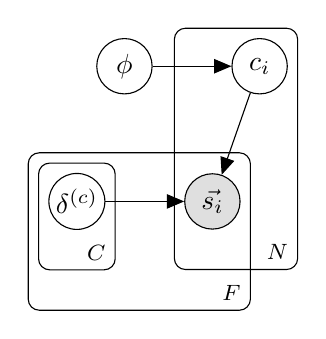
\begin{tikzpicture}
\node[latent] (c) {$c_{i}$};
\node[obs, below=of c, xshift=-0.6cm] (s) {$\vec{s_{i}}$};
\node[latent, left=of c] (phi) {$\phi$};
%\node[const, left=of phi] (beta) {$\beta$};
\node[latent, left=of s] (delta) {$\delta^{(c)}$};
%\node[const, left=of delta] (gamma) {$\gamma$};

\edge {phi}{c};
\edge {delta, c}{s};
%\edge {beta}{phi};
%\edge {gamma}{delta};

\plate {nutt}{(c)(s)}{$N$};
\plate {cvalue}{(delta)}{$C$};
\plate {fvalue}{(delta)(s)(cvalue)}{$F$};
\end{tikzpicture}
\end{center}
%\end{figure}
\end{minipage}
\hspace{0.5cm}
\begin{minipage}[b]{0.45\linewidth}	
%\begin{figure}[H]
\begin{center}
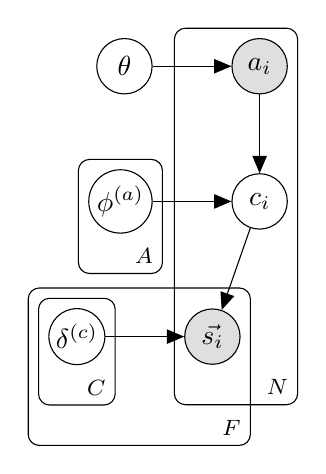
\begin{tikzpicture}
\node[obs] (a) {$a_{i}$};
\node[latent, left=of a] (theta) {$\theta$};
%\node[const, left=of theta] (alpha) {$\alpha$};
\node[latent, below=of a] (c) {$c_{i}$};
\node[obs, below=of c, xshift=-0.6cm] (s) {$\vec{s_{i}}$};
\node[latent, left=of c] (phi) {$\phi^{(a)}$};
%\node[const, left=of phi] (beta) {$\beta$};
\node[latent, left=of s] (delta) {$\delta^{(c)}$};
%\node[const, left=of delta] (gamma) {$\gamma$};

\edge {theta}{a};
%\edge {alpha}{theta};
\edge {phi, a}{c};
\edge {delta, c}{s};
%\edge {beta}{phi};
%\edge {gamma}{delta};

\plate {nutt}{(a)(c)(s)}{$N$};
\plate {avalue}{(phi)}{$A$};
\plate {cvalue}{(delta)}{$C$};
\plate {fvalue}{(delta)(s)(cvalue)}{$F$};
\end{tikzpicture}
\end{center}
\end{minipage}
\caption{The  \distlearner{} (left) and \praglearner{} (right)}\label{fig:engcl:model}
\end{figure}




Both models assume that there are three clause type categories, \diis{}, that explain the distribution of a set of morpho-syntactic properties in the input. This is shown in the graphical illustrations in Figure~\ref{fig:engcl:model} as the morpho-syntactic properties $\vec{s_{i}}$ being conditioned on the clause type variable $\vec{c_{i}}$. The \plearnerabbr{} model additionally assumes that there are four speech act categories (assertions, questions, requests/commands, or some other speech acts such as exclamatives), and that this pragmatic information helps to identify the clause type category. This is shown in the graphical representation as the variable $c_{i}$ being conditioned on the variable $a_{i}$ (for speech act). 

In both models, the clause type variable $c_{i}$ follows a multinomial distribution with a parameter $\phi$. This parameter is assumed to have a uniform Dirichlet prior $\mbox{Dir}(1,1,1)$. This means that it is equally likely \emph{a priori} for a sentence to be a declarative, interrogative or imperative. For the model simulating the \distlearner{}, the parameter $\phi$ represents the probability that a sentence $i$ is a declarative, interrogative, or imperative. As the \plearnerabbr{} model assumes that the speech act category $a_{i}$ of the utterance expressed by the sentence informs the learner of the clause type category, so the parameter $\phi^{(a)}$ in this model represents the probability that a sentence $i$, which expresses the speech act $a_{i}$, is a declarative, interrogative, or imperative. 

In the \plearnerabbr{} model, the speech act variable $a_{i}$ follows a multinomial distribution with parameter $\theta$. This parameter represents the probability that the speech act expressed by the sentence $i$ is an assertion, question, request/command, or some other speech act. This parameter also has a uniform Dirichlet prior $\mbox{Dir}(1,1,1,1)$, meaning that we assume that it is equally likely \emph{a priori} that the sentence $i$ expresses an assertion, question, request/command, or some other speech act.

In both models, morpho-syntactic properties are represented by a vector of Bernoulli variables $\vec{s_{i}}$, and $\vec{s_{i}}$ is conditioned on $c_{i}$. 
The number of morpho-syntactic properties included is represented by a vector $F$, and the properties are the same as the ones in the corpus study listed in Table~\ref{tab:eng-cl:formal-schema} in Section~\ref{sec:engcl:corpus:schema}. Each $s^{(F)}_{i}$ in $\vec{s_{i}}$ takes the value 1 if the sentence contains the property, and 0 otherwise. $s^{(F)}_{i}$ is conditioned on the parameter $\delta^{(c, F)}$, which represents the probability of observing a given morpho-syntactic property in a particular clause type category. 
This parameter is assumed to have a uninformative uniform $\mbox{Beta}(1,1)$ prior, meaning that \tit{a priori}, it is equally likely for a particular property to be present or absent in a clause type category. 


Tables~\ref{tab:engcl:baseline-variables} and ~\ref{tab:engcl:target-variables} summarize the notation and statistical assumptions for the two models. 

\begin{table}[H]
    \centering
    \begin{tabular}{cl}
    \hline
    \hline
        $c_{i}$ &  Clause type, declarative, interrogative, imperative\\
        &$\vec{\phi^{a}} \sim \mbox{Dir}(1,1,1)$\\        
        & $ c_{i} \sim  \mbox{Multinomial}(\vec{\phi})$;\\
\hline
        $\vec{s_{i}}$ &  Morpho-syntactic properties; \\
        & See Table~\ref{tab:eng-cl:formal-schema} for the full list of features included \\
        &$\delta\sim \mbox{Beta}(1,1)$\\        
        & $s_{i}^{(F)} \sim \mbox{Bernoulli}(\delta^{(c)})$ \\
    \hline
    \hline
    \end{tabular}
    \caption{Variables in \distlearner{} model, their distribution, and explanation}
    \label{tab:engcl:baseline-variables}
\end{table}


\begin{table}[H]
    \centering
    \begin{tabular}{c|l}
    \hline
    \hline
        $a_{i}$ & Speech Act: \\
        	  &Assertion, Question, Request/Command, Other\\
          & $\vec{\theta} \sim \mbox{Dir}(1,1,1,1)$\\
          & $ a_{i} \sim \mbox{Multinomial}(\vec{\theta})$;\\

\hline
         $c_{i}$ &  Clause Type:\\
        & Declarative, Interrogative, Imperative\\
        &$\vec{\phi^{(a)}} \sim \mbox{Dir}(1,1,1)$\\
        &  $c_{i} \sim  \mbox{Multinomial}(\vec{\phi^{(a)}})$;\\
\hline
        $\vec{s_{i}}$ &  Set of morpho-syntactic properties; \\
        $s_{i}^{(F)}$ &  property $F$ in the set;  \\
        &$\delta\sim \mbox{Beta}(1,1)$\\        
        & $s_{i}^{(F)} \sim \mbox{Bernoulli}(\delta^{(c)})$ \\
    \hline
    \hline
    \end{tabular}
    \caption{Variables of the \plearnerabbr{} model, their distributions, and explanations}
    \label{tab:engcl:target-variables}
\end{table}


\subsection{Inferences}
\label{sec:engcl:model:infer}

The task of both learners is then to infer the category assignment of the clause type variable (i.e. is the sentence a declarative, interrogative, or imperative) from observations of morpho-syntactic properties of the sentence. The \plearnerabbr{} learner additionally observes speech act information and assumes it is related to clause type. 

I applied Gibbs sampling (\cite{geman1984gibbs}), a form of a Markov chain Monte Carlo sampler to sample from the posterior distribution of clause type category assignments. The sampling algorithm of the two learners are detailed below. In the following algorithms, $\vec{c}$ represent the set of clause type assignments in the corpus. The variable $\vec{a}$ represents the set of all speech act values in the corpus; $\vec{S}$ represents all values in the corpus for the set of morpho-syntactic properties. The subscript $i$ represents the current sentence, and $-i$ represents all values of a variable except the current sentence (for example, $c_{i}$ represents the clause type assignment of the current sentence, and $c_{-i}$ represents the clause type assignments of all sentences in the corpus except the current one).

\begin{comment}
\tbf{The \dlearnerabbr{} model:} We first randomly initialized assignments of $c_{i}$ for each sentence with three categories (representing declaratives, interrogatives, and imperatives). 

\tbf{The \plearnerabbr{} model:} The algorithm first randomly initializes assignments of $c$ for all sentence with three values (representing declaratives, interrogatives, and imperatives). Then it sweeps to update values of $c_{i}$. The posterior predictive probability can be computed using Bayes' Rule as follows:

\begin{equation}
p(c_{i}| c_{-i}, \vec{a}, \vec{S_{i}},\phi, \delta) = \frac{p(\vec{S_{i}}| \vec{c}, \delta)\ p(c_{i}|, c_{-i}, \phi,\vec{a})}{\Sigma_{c_{i}'}p(\vec{S_{i}}| \vec{c'}, \delta)\ \ p(c_{i}'|, c_{-i}, \phi, \vec{a})}
\end{equation}

%The prior distribution $ p(c_{i}|, c_{-i}, \vec{a})$ follows a Multinomial distribution with the parameter $\phi$, which in turn follows a Dirichlet distribution with parameter $\beta$:

\begin{equation}
\begin{split}
 p(c_{i}|\phi_{a_{i}} ,\beta, c_{-i},  \vec{a})  =& \int p(c_{i}|\phi_{a_{i}}, \beta) p(\phi_{a_{i}}| c_{-i}, \beta)d\phi_{a_{i}} \\
= & \int \prod_{k}\ \phi_{k}^{1^{c_{i}=k}}\ \frac{\Gamma(\sum_{k}\beta_{k})}{\prod_{k}(\Gamma(\beta_{k}))}\prod_{k} \phi_{k}^{\beta_{k}-1}d\phi
\end{split}
\end{equation}

The likelihood term:

\begin{equation}
\begin{split}\label{p(s|c)}
p(\vec{S_{i}}| \vec{c}, \delta, \gamma) = & \prod_{F} p(s^{(F)}_{i}|\vec{c}^{(F)}, \delta, \gamma)\\%split to each feature of S
= &\prod_{F}\int p(s^{(F)}_{i}|c_{i}^{(F)}, \delta^{(F)}_{c_{i}}, \gamma^{(F)})\ p(\delta^{(F)}_{c_{i}}|c^{(F)}_{-i}, s^{(F)}_{-i},\gamma^{(F)}) d\delta_{c_{i}}\\%predicative posterior distribution
=& \prod_{F}\int \prod_{k} \delta^{1^{s_{i}=k}}_{k}%expand p(s_{i})
\prod_{k} \delta_{k}^{\gamma_{k}-1}  %expand p(delta)
\frac{\Gamma(\sum_{k}(\gamma_{k}))}{\prod_{k}(\Gamma(\gamma_{k}))}%normalizing constant for p(delta)
d\delta_{c_{i}} 
\end{split}
\end{equation} 
\begin{equation}
\begin{split}
p(\vec{S_{i}}| \vec{c}, \delta, \gamma)=&\prod_{F}\frac{\Gamma(\sum_{k}(\gamma_{k}))}{\Gamma(\gamma_{s_{i}})\prod_{k\neq s_{i}}(\Gamma(\gamma_{k}))}%old NC
\frac{\Gamma(\gamma_{s_{i}}+1)\prod_{k\neq s_{i}}(\Gamma(\gamma_{k}))}{\Gamma(\sum_{k}(\gamma_{k})+1)}\\%separate out k from s_{i}
=&\prod_{F}\frac{\gamma_{s_{i}}}{\sum_{k}(\gamma_{k})}\\%reduce
=&\prod_{F}\frac{\gamma_{0}+n_{s_{i}}}{(\gamma_{0}+n_{s_{i}})(\gamma_{0}+n_{c_{i}}-n_{s_{i}})}\\%update function
=& \prod_{F}\frac{\gamma_{0}+n_{s^{F, c_{i}}_{i}}}{2\gamma_{0}+n^{F}_{c_{i}}}
\end{split}
\end{equation}
\end{comment}
   %Assume $\beta_{k}$ is the value of $\beta$ for when $c = k$ (i.e. the clause type assignment is $k$), $n_{c_{i}}$ as the number of observations of $c=c_{i}$ so far, and  $n_{c_{i}}^{(k)}$ is the number of observations of other values of $c$ 

For both models, we first randomly initialize values of $c_{i}$ for each sentence with three categories (representing declaratives, interrogatives, and imperatives). After initialization, the \dlearnerabbr{} sweeps to update current $c_{i}$ with the posterior distribution specified in Equation~\ref{eq:engcl:base}, and the \plearnerabbr{} updates with Equation~\ref{eq:engcl:target}. The likelihood term of both models is the conditional probability $p(\vec{S}|\vec{c})$, but the prior terms differ, as for the \plearnerabbr{} the probability of the assignment of $c_{i}$ is conditioned on the speech act values $\vec{a}$. 

\begin{equation} \label{eq:engcl:base}
p(c_{i}| c_{-i}, \vec{S_{i}},\phi, \delta) \propto p(\vec{S_{i}}| \vec{c}, \delta)\ p(c_{i}|, c_{-i}, \phi)
\end{equation}

\begin{equation} \label{eq:engcl:target}
p(c_{i}| c_{-i}, \vec{a}, \vec{S_{i}},\phi, \delta) \propto p(\vec{S_{i}}| \vec{c}, \delta)\ p(c_{i}|, c_{-i}, \phi,\vec{a})
\end{equation}

%uses the the observed values of morpho-syntactic properties to infer for the current utterance and the values of $C$ of other sentences to calculate a posterior distribution over new category assignments for the current sentence, and then re-sample the new value of $C$ from this posterior probability distribution. 


For each model, I ran the chain for 5000 iterations and analyzed the last sample. Each learner was simulated 10 times. 


\subsection{Simulations with infant-directed speech}
\label{sec:engcl:model:results}

The data for this model were taken from the annotated dataset reported in Section~\ref{sec:engcl:corpus}. The labels of speech acts and morpho-syntactic observations were used as input to the models, and the true labels of clause type were used to evaluate the performance of the models. As the learners need to use the surface features of sentences to learn about clause-level properties, instead of one-noun utterances or utterances of only injectives, we eliminated from the dataset sentences that do not contain a verb or an auxiliary. In total, $3923$  sentences were fed into the models.


Figure~\ref{fig:compare-rand} shows the rand scores of the two models over 10 iterations, and in comparison with the rand scores of the two multinomial logistic regression models ran in Section~\ref{sec:engcl:corpus:supervised}. 
This score was calculated by taking all pairs of samples and counting ones that are assigned to the same or different clusters in two clusterings to measure the similarity between the clusterings (\cite{rand1971}). This score ranges between 0 and 1, where a higher score indicates better performance. 

Overall, the \plearnerabbr{} model substantially outperforms the \dlearnerabbr{} model. The pragmatic information led to an improvement from an average 0.74 rand score to an average of 0.87 rand score, bringing the model up to the level of supervised performance. This suggests that pragmatic information is crucial for learning the clustering of clause type information. 


\begin{figure}[H]
    \centering
    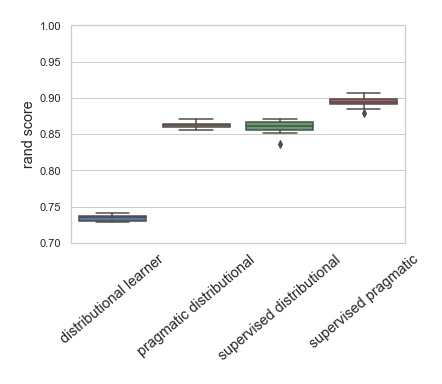
\includegraphics[width=0.6\textwidth]{figures/compare-rand.jpg}
    \caption{Comparing all four learners (distributional, pragmatic distributional, supervised distributional, supervised pragmatic) by rand score }
    \label{fig:compare-rand}
\end{figure}


\subsubsection{The \dlearnerabbr{} model}
\label{sec:engcl:model:results:d}
For a model to be successful it is not sufficient that it categorizes its input sentences into \emph{any} three categories. The three categories should correspond to the sets of actual declaratives, actual interrogatives and actual imperatives. That is, for example, if in the classification learned by the model, the actual declaratives are split across two categories, the model has not learned to cluster by clause type.
Turning to the profile of each cluster identified by the \dlearnerabbr{} model, Figure~\ref{fig:baseline-heatmap} shows the proportion of \diis{} in each identified cluster, and Figure~\ref{fig:baseline-heatrev} shows the proportion of sentences clustered together. In other words, Figure~\ref{fig:baseline-heatmap} shows whether each cluster mostly consists of one clause type, and Figure~\ref{fig:baseline-heatrev} shows whether each clause type is put in one cluster.  



\begin{figure}[H]
    \centering
    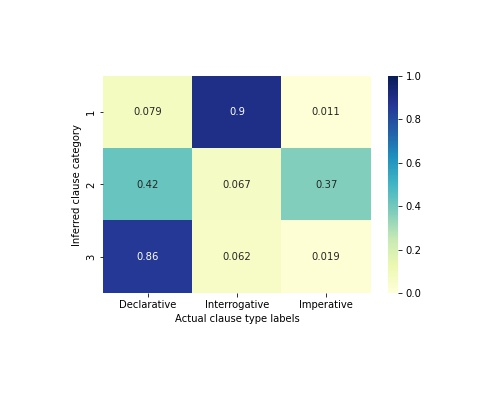
\includegraphics[width=0.7\textwidth]{figures/baseline-heatmap.jpg}
    \caption{The proportion of \diis{} in each of the three clusters identified by the \dlearnerabbr{} model}
    \label{fig:baseline-heatmap}
\end{figure}


\begin{figure}[H]
    \centering
    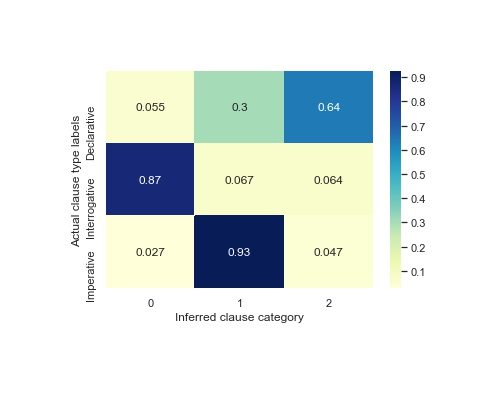
\includegraphics[width=0.7\textwidth]{figures/baseline-heatrev.jpg}
    \caption{The proportion of actual \diis{} clustered in one category}
    \label{fig:baseline-heatrev}
\end{figure}


Overall, Figure~\ref{fig:baseline-heatmap} shows that the \dlearnerabbr{} model identifies an interrogative cluster and a declarative cluster. Cluster~$0$ mostly contains interrogative clauses, as 90\% of sentences in this cluster are interrogative; Cluster~$2$ is mostly declarative, and 86\% of the data in this cluster are declaratives. Cluster~$1$ is split between declaratives and imperatives. Figure~\ref{fig:baseline-heatrev} shows that 87\% of interrogatives and 93\% of imperatives are clustered together in Cluster~$0$ and $1$ respectively. While most of declaratives are classified in Cluster~$2$, a proportion is classified in Cluster~$1$.

These results seem to suggest that the \dlearnerabbr{} found two out of three clause types, but how do these clause types look like? Did the model find the right morpho-syntactic properties to associate with each clause type? Figure~\ref{fig:baseline-syncluster} plots the morpho-syntactic profile of each cluster identified by the \dlearnerabbr{}. Darker colors represent sentences with the morpho-syntactic property, and lighter colors represent sentences without the property. 

\begin{figure}[H]
    \centering
    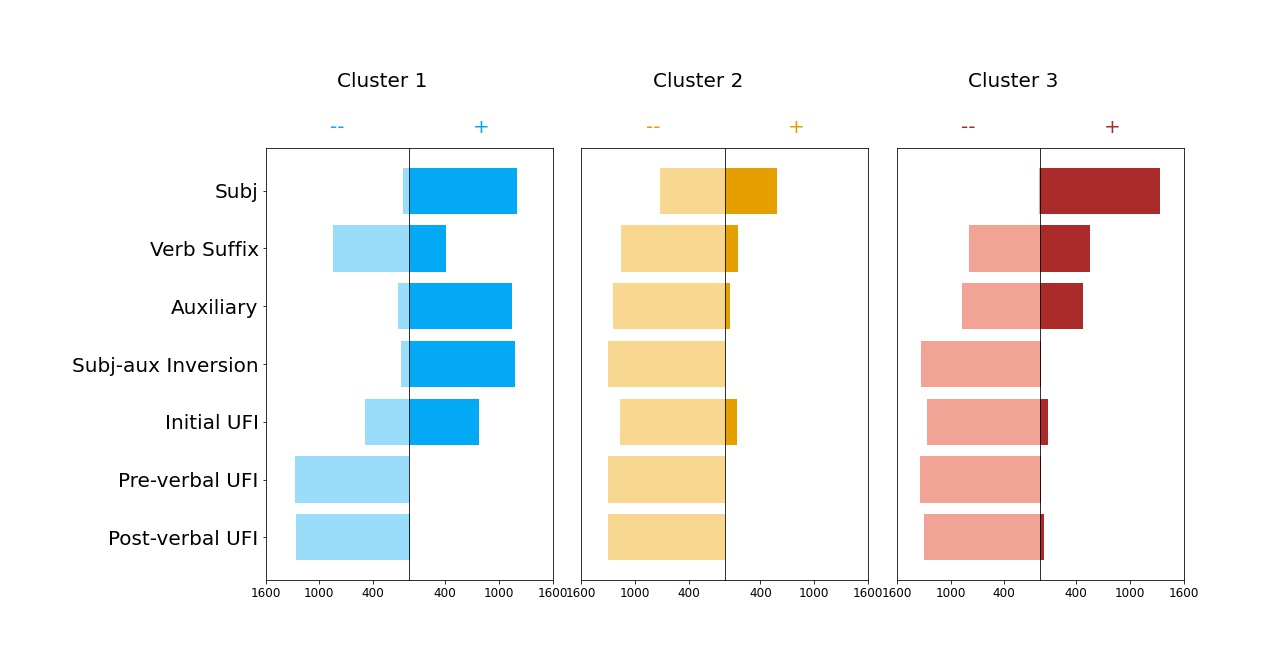
\includegraphics[width=1\textwidth]{figures/baseline-syncluster.jpg}
    \caption{The number of sentences with/without certain formal features in each cluster (Cluster 0 $\sim$ Interrogatives, Cluster 1 $\sim$ Imperatives, Cluster 2 $\sim$ Declaratives), darker colors represent the number of sentences with the feature. UFI stands for Unknown Functional Item (e.g. \twh{}), see Table~\ref{tab:eng-cl:formal-schema} for details.}
    \label{fig:baseline-syncluster}
\end{figure}

We can see that Cluster~$0$, which is 90\% interrogative clauses, is associated with [+int] morpho-syntactic properties such as subject-auxiliary inversion and sentence-initial unknown functional item (e.g. \twh{}). 

The other two clusters are not as ideal. Cluster~$1$ consists of a mix of imperative sentences and simple declarative sentences. While it appears that the cluster mostly consists of sentences with bare verb stem, which is characteristic for imperatives in English, but a quick look at the sentences show that it also includes declaratives with these properties as well:

\bex{engcl:baseline:cluster1-dec}
 I love school. \hfill Mother of Lily, Session 010423
\eex

The sentence is clustered together with imperatives like \tit{Take the bottle!} by the model. Ambiguous sentences like \ref{engcl:baseline:cluster1-amb} are also put in this cluster:
\bex{engcl:baseline:cluster1-amb}
Wanna read your little Tigger book? \hfill Mother of Violet, Session 010407
\eex

Moreover, compare to the distribution of morpho-syntactic features of imperatives in English in Figure~\ref{fig:real-syncluster}, this cluster seems to have more sentences with subjects. It seems that instead of finding a cluster for imperatives and declaratives, the model puts too much weight on the lack of subjects in a sentence, so any sentences without subjects are in Cluster~$1$. 

\begin{comment}
A multinomial logistic regression model was performed to further probe into the morpho-syntactic profile of each cluster, with the three
clusters as dependent variable (with Cluster~$2$ as the default), and the set of morpho-syntactic properties as independent variable. The results are shown in Table~\ref{tab:baseline-synstats} (details of the regression model, coefficients, and $p$-values are reported in Appendix~\ref{appx:engcl}).


\begin{table}[H]
\begin{center}
\begin{tabular}{c|p{10cm}}
\hline
Clusters (default Cluster~$2$) & Morpho-syntactic cues\\
\hline \hline
Cluster~$0$ & +auxiliary, +subject-auxiliary inversion, +sentence-initial UFI\\
\hline
Cluster~$1$  & $-$subject, $-$verb suffix\\
\hline \hline
\end{tabular}
\end{center}
\label{tab:baseline-synstats}
\end{table}%

The table shows that while 
\end{comment}

Overall, the \dlearnerabbr{} model fails to identify the clause type clustering in English, and fails to identify the characteristic morpho-syntactic properties for these clause types. 


\subsubsection{The \plearnerabbr{} model}
\label{sec:engcl:model:results:p}

Figure~\ref{fig:target-heatmap} shows the proportion of \diis{} in each identified cluster, and Figure~\ref{fig:target-heatrev} shows the proportion of sentences clustered together. 
\begin{figure}[H]
    \centering
    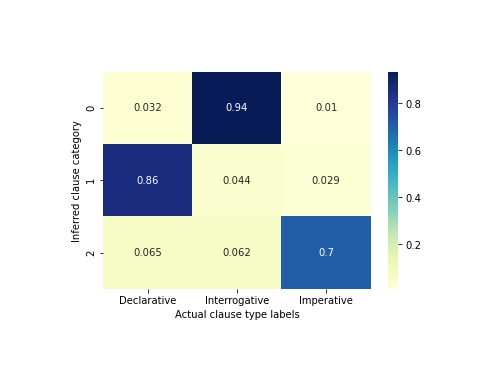
\includegraphics[width=0.7\textwidth]{figures/target-heatmap.jpg}
    \caption{The proportion of \diis{} in each of the three clusters identified by the \plearnerabbr{} model}
    \label{fig:target-heatmap}
\end{figure}




\begin{figure}[H]
    \centering
    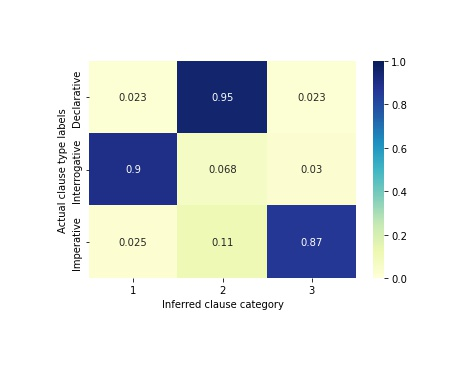
\includegraphics[width=0.7\textwidth]{figures/target-heatrev.jpg}
    \caption{The proportion of actual \diis{} clustered in one category}
    \label{fig:target-heatrev}
\end{figure}
%Rand comparison

%confusion matrix

We can see that the \plearnerabbr{} model clearly identifies a declarative, an interrogative, and an imperative cluster: 94\% of Cluster~$0$ are interrogatives, 86\% of Cluster~$1$ are declaratives, and 70\% of Cluster~$2$ are imperatives. The three clause types in English are also mostly clustered together by the model: 95\% of declaratives, 90\% of interrogatives, and 87\% of imperatives are clustered together in Cluster~$1$, $0$, $2$ respectively. In contrast to \dlearnerabbr{}, this learner is able to find the right clause types in English.


Figure~\ref{fig:target-syncluster} shows the morpho-syntactic profile of each cluster identified by the \plearnerabbr{}. 

\begin{figure}[H]
    \centering
    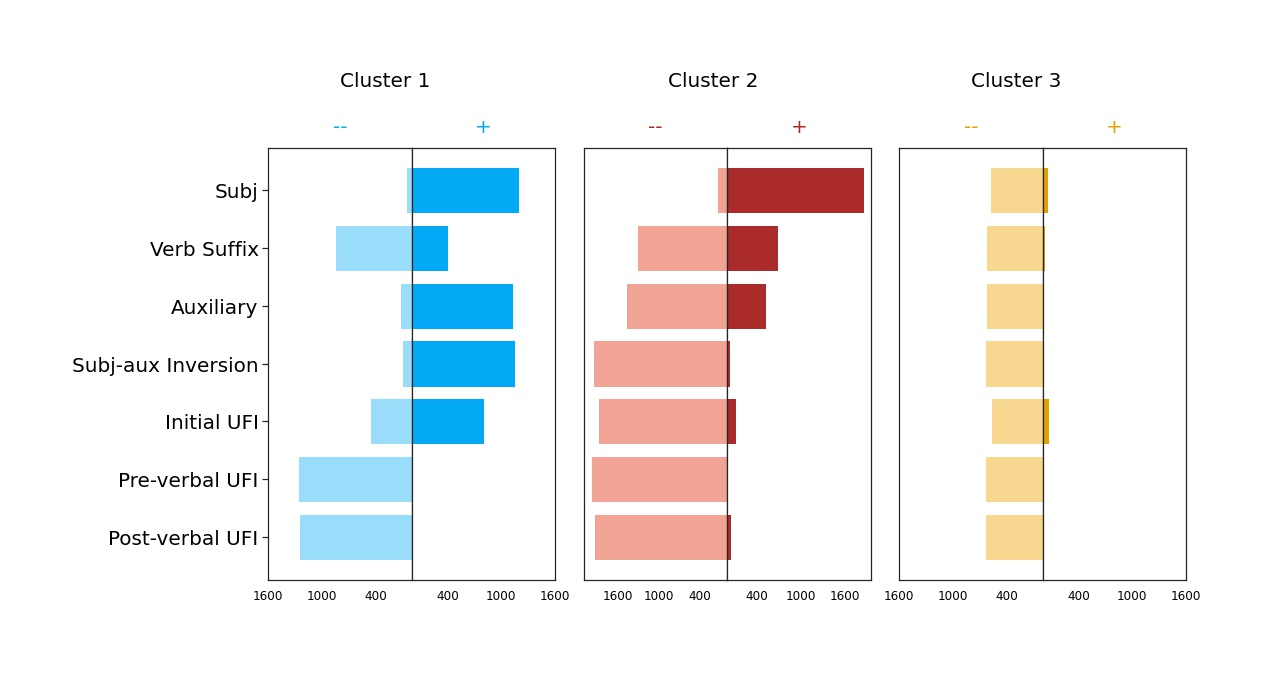
\includegraphics[width=1\textwidth]{figures/target-syncluster.jpg}
    \caption{The number of sentences with/without a formal propertyin each cluster (Cluster 0 $\sim$ Interrogatives, Cluster 1 $\sim$ Declaratives, Cluster 2 $\sim$ Imperatives), darker colors represent the number of sentences with the property, lighter colors represent sentences without the property.}
    \label{fig:target-syncluster}
\end{figure}

The profile of the three clusters resembles the profile of \diis{} in our corpus study (Figure~\ref{fig:real-syncluster}). The cluster for interrogatives has more sentences with subject-auxiliary inversion and clause-initial unknown functional items (e.g. \twh{}), and the cluster for imperatives is characterized by the lack of subjects and verb suffixes. 

\begin{comment}
Table~\ref{tab:target-synstats} summarises the three logistic regression models with each of the clusters as dependent variable, and the set of formal features (+/- verb and pre-verbal UFI are excluded, due to low variance) as independent variables.  
\begin{table}[H]
\begin{center}
\begin{tabular}{r|l|l|l}
\hline
 & Cluster~$0$   & Cluster~$1$   &  Cluster~$2$ \\
 & $\sim$ Interrogatives  & $\sim$Declaratives  & $\sim$ Imperatives \\
 \hline\hline
constant & -6.3*** & -1.44*** & 1.95*** \\
\hline
Subject & 0.9** & 4.32*** & -4.75*** \\
\hline
Verb Morphology & -0.31 & 1.66***  & -3.08*** \\
\hline
Auxiliary & 2.66***  & -0.85*** & -2.14*** \\
\hline
Subject-Aux Inversion &5.99*** & -5.83*** & -56.79 \\
\hline
Sentence-initial UFI & 3.65*** & 0.38* & 0.72** \\
\hline
Post-verbal UFI & -0.43  & 0.5  & -1.12 \\
\hline \hline
\end{tabular}
\end{center}
\caption{Results from the three logistic regression models with each of the clusters as the dependent variable and the morpho-syntactic features as independent variables; asterisks represent the significance level: ‘***’ 0.001 ‘**’ 0.01 ‘*’ 0.05 ‘.’ 0.1 ‘ ’ 1}
\label{tab:target-synstats}
\end{table}%
\end{comment}
% \begin{figure}[H]
%     \centering
%     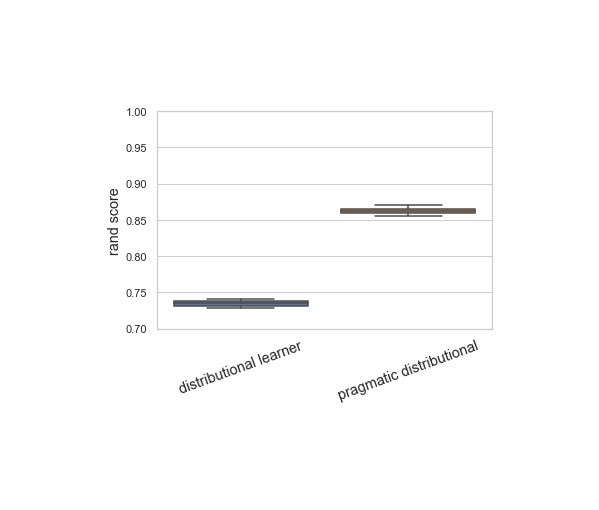
\includegraphics[width=0.6\textwidth]{figures/target-base-rand.jpg}
%     \caption{Comparing the pragmatic distributional learner and the distributional learner by rand score }
%     \label{fig:target-base-rand}
% \end{figure}

\subsubsection{Interim Summary}
\label{sec:engcl:model:results:summary}

Using data from infant-directed speech in English, our models simulate the \distlearner{} and the \praglearner{}.
 We found that the \plearnerabbr{} model performs much better than the \dlearnerabbr{} model; it successfully identifies three clause clusters roughly corresponding to the three major clause types in English. In contrast, the \dlearnerabbr{} model fails to find the right clustering, collapsing declaratives and imperatives. These results suggest that pragmatic information is essential for children to solve the clustering problem for clause types. But how much pragmatics does the learner need? Recall from Chapter \ref{chap:introduction} that assuming \emph{too much} pragmatics to be available to learners might catch us in a circularity. Considering the fact that 18-month-olds' pragmatic skills might still be developing, it is likely that they are not able to perfectly identify the speech act information of some utterances, and thus the pragmatic information available to the learner might be rather noisy. To probe deeper into this question, I now turn to simulated pragmatic learners with noisy speech act information. Studying such learners will allow us to investigate how much pragmatics is need to solve the clustering problem. 



\subsection{Simulating noisy pragmatic information} 
\label{sec:engcl:model:noisy}
%how noise is generated
As we have seen in the last section, pragmatics information is crucial for clause type clustering. In this series of simulations, I manipulated the amount of noise in the speech act information that the \plearnerabbr{} model takes as input. Instead of feeding the model true speech act labels, I replaced a percentage of the data with random speech act labels to simulate the situation where the learner randomly guess the speech act for a proportion of the utterances they hear. Each simulation was run 10 times. 

Figure~\ref{fig:noisy-rand-compare} shows the simulations with 0-100\% noise. The performance of the \dlearnerabbr{} model in our last simulation is marked by the dotted line. As can be seen, the \plearnerabbr{} learner outperforms the \dlearnerabbr{} learner up until there is around 80\% of noise in speech act, and even at 80\% level there are iterations that outperforms the \dlearnerabbr{}. This suggests that a little pragmatics goes a long way, as the learners with noisy pragmatic information still outperforms the one without. 

\begin{figure}[H]
    \centering
    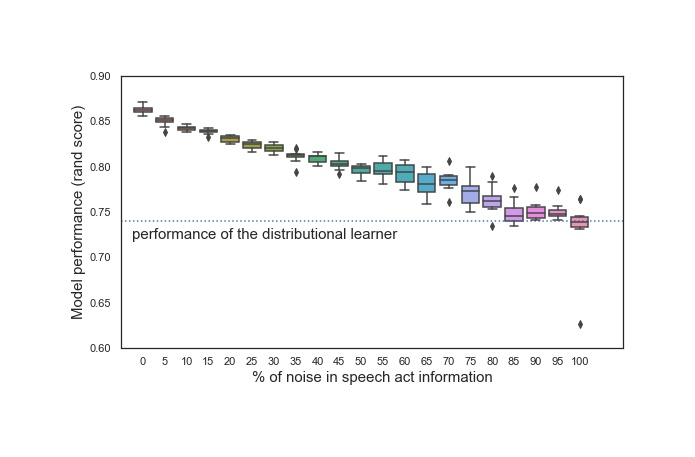
\includegraphics[width=1\textwidth]{figures/noisy-rand-compare.jpg}
    \caption{Performance of the \plearnerabbr{} model with different levels of noise in the speech act information; dotted marks the rand score of the \dlearnerabbr{} learner}
    \label{fig:noisy-rand-compare}
\end{figure}


Looking at the learner at maximum noise level, we can see that the \plearnerabbr{} reverts back to the performance of the \dlearnerabbr{} in that it fails to identify a cluster for declaratives (Figure~\ref{fig:noisy100-heatmap}. Similar to the distributional learner, the cluster containing most imperatives also contains many declaratives (\ref{fig:noisy100-heatrev}). 

\begin{figure}[H]
    \centering
    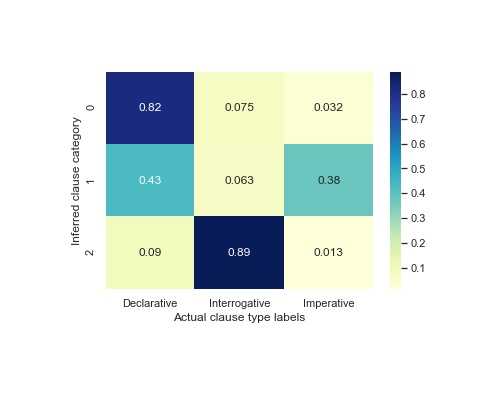
\includegraphics[width=0.7\textwidth]{figures/noisy100-heatmap.jpg}
    \caption{The proportion of \diis{} in each of the three clusters (100\% noise in speech act information) }
    \label{fig:noisy100-heatmap}
\end{figure}

\begin{figure}[H]
    \centering
    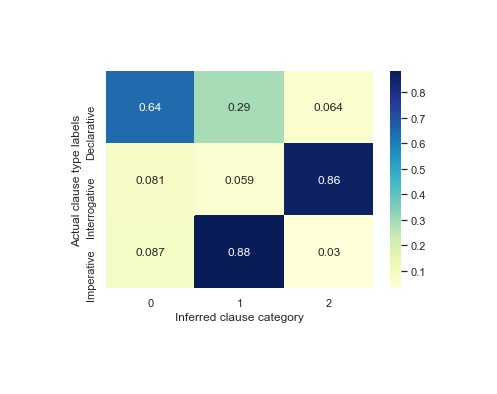
\includegraphics[width=0.7\textwidth]{figures/noisy100-heatrev.jpg}
    \caption{The proportion of actual \diis{} clustered in one category}
    \label{fig:noisy100-heatrev}
\end{figure}

Looking at the morpho-syntactic profile of this model with random speech act information, we again see that it behaves like the \dlearnerabbr{} model, and fails to identify the properties of English imperatives and declaratives.

\begin{figure}[H]
    \centering
    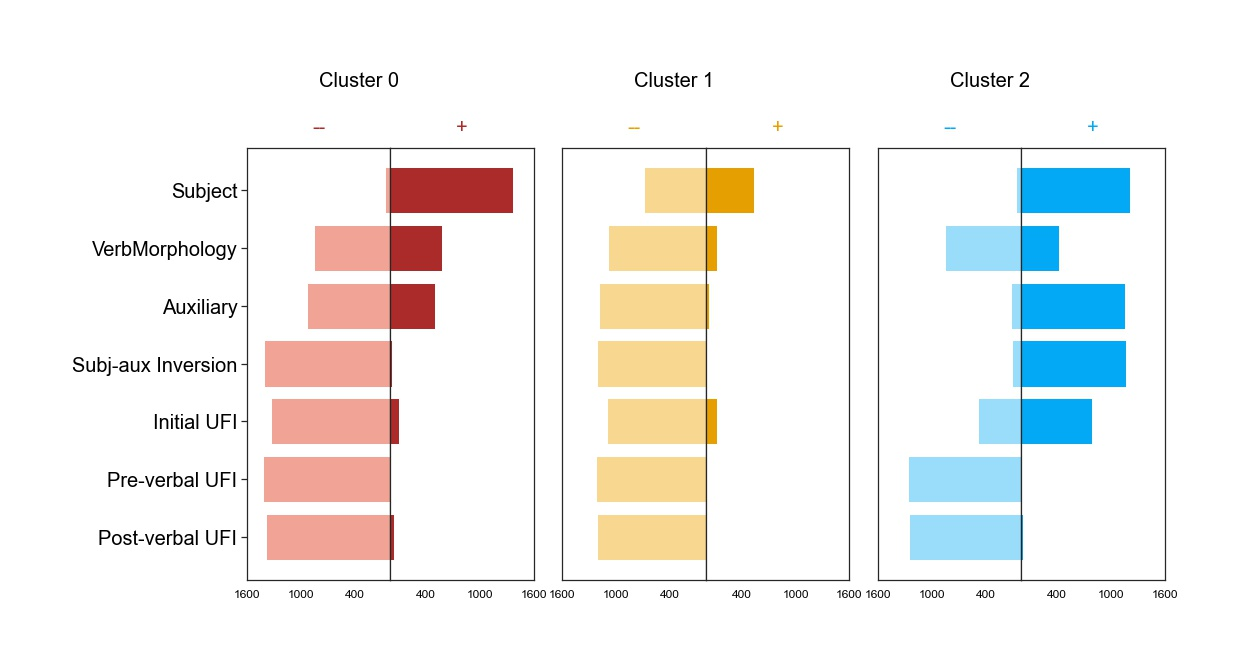
\includegraphics[width=1\textwidth]{figures/noisy100-syncluster.jpg}
    \caption{The number of sentences with/without certain formal features in each cluster (Cluster 0 $\sim$ Interrogatives, Cluster 1 $\sim$ Imperatives, Cluster 2 $\sim$ Declaratives), darker colors represent the number of sentences with the feature.}
    \label{fig:noisy100-syncluster}
\end{figure}

Results from our simulations suggest that morphosyntax is not sufficient to solve the clustering problem, and a small amount of pragmatic information is necessary.

\section{Discussion}
\label{sec:engcl:discussion}

This chapter investigates how 18-month-olds learn to identify the three clause types in English. Our corpus study provides evidence suggesting that the information that children need to solve the clustering and labeling problems for acquiring clause types is present in their input. Parents use clause types systematically, and the three clause types are predominantly mapped to their canonical functions (declaratives to assertions, interrogatives to questions, imperatives to requests/commands) despite the presence of the theoretically expected exceptions to this mapping. The three clause types also show systematically different formal profiles in the input: compared to declaratives, interrogatives are more likely to have auxiliaries, subject-auxiliary inversion, and clause-initial functional items like \twh{}, which are characteristic of [+int] of $C^{0}$ in English; imperatives are more likely to not have subjects or verb suffixes, which is characteristic of [+imp].


I then investigated the extent to which learners need to rely on pragmatic information (i.e., knowing what speech act a given utterance of sentence is conveying), to solve not just labeling, but the clustering itself. I built two Bayesian clustering models simulating a \distlearner{} (\dlearnerabbr{}) and a \praglearner{} (\plearnerabbr{}). I found that morpho-synatctic information is not sufficient for finding the right clause type clustering and a small amount of pragmatic information is necessary, as the \plearnerabbr{} learner outperforms the \dlearnerabbr{} when we ran the two models with the annotated dataset from our corpus study. In addition, a small amount of pragmatics might suffice; even with 80\% of noise, the speech act information still helps improve the performance of the model. So even if the speech act information is not perceived veridically for all utterances, learners can still enjoy its benefits.

Now that we have established the importance of pragmatics, and that a small amount of pragmatics might suffice, the question then is, is there any information in the non-linguistic behavior of parents that signals the speech act of an utterance? We will turn to these questions in Chapter~\ref{chap:eng-sp}.


%Our next question is then, what about other languages? As we have discussed in Chapter~\ref{chap:background}, languages differ in the formal features of each clause type, and learners need to discover the correlation from input. The distributional learner for English still have some success with clustering, identifying interrogative clauses. However, maybe the formal features are not as informative in other languages. In the next chapter, we will turn to Mandarin learners, and test the two learners with Mandarin input data. 

\chapter{Learning to identify clause types in Mandarin}
\label{chap:man-cl}

In this chapter, we will explore how Mandarin-acquiring children learn clause typing. As we have seen from last chapter, pragmatic information is crucial for finding the right clause type clustering. We find that a learner must have access to some pragmatic information in order to find the right clause types but this learner can succeed with very limited access to pragmatic information. 

As Mandarin [+int] and [imp] have different properties, would they be able to infer surface forms associated with these features from the input? Is pragmatics also crucial for Mandarin-acquiring children? How much pragmatics is required? In this chapter, I address these questions computationally, and found that surface morpho-syntactic features alone cannot help learners cluster sentences into the three clause types, and pragmatics is also needed. 

This chapter is organized as follows: we will review the properties of Mandarin [+int] and [imp], and children's knowledge regarding these properties. I then report results from a corpus study for Mandarin-speaking parents' input to children in  ~\ref{sec:mancl:corpus}. The data from the corpus study was used to simulate the two learners, \distlearner{} and \praglearner{}.  %

\section{Background}
\label{sec:mancl:bg}
\subsection{Clause types in Mandarin}
\label{sec:mancl:bg:theory}


In Mandarin, the [+int] value in $C^{0}$ does not trigger movements, but instead shows up in surface form as \twh-phrases, sentence final \tit{ma}, and A-not-A. For \twh-interrogatives, Mandarin \twh-phrases (\citealt{huang1982, cheng1991} among many others) do not need to be fronted to clause-initial position. Compare the declarative sentence in (\ref{bg-syn:dec-man}) with the \twh-interrogative in (\ref{bg-syn:wh-man}), the \twh-phrase \tit{shenme} occurs in the same position in the interrogative (\ref{bg-syn:wh-man}) as the noun phrase \tit{zaocan} in (\ref{bg-syn:dec-man}). 


%\begin{minipage}[t]{0.45\linewidth}	
\bex{bg-syn:dec-man}
\gll Xiaoxiao	chi-le zaocan.\\
Xiaoxiao eat-\Asp{} breakfast \\
``Xiaoxiao ate breakfast.''
\eex
\bex{bg-syn:wh-man}
\gll Xiaoxiao	chi-le \tun{shenme}.\\
Xiaoxiao eat-\Asp{} what \\
``What did Xiaoxiao eat?''
\eex


Interrogativity might also have effects on prosody. As mentioned before, \twh-phrases in Mandarin can be interrogative or indefinite (\ref{bg-syn:ambwh}), but interrogative \twh{} is normally associated with prosodic prominence (\cite{hu2002prosody, dong2009, yangyang2018} a.o.).

\bex{bg-syn:ambwh}
\gll Xiaoxiao	mei	chi	\tun{shenme}\\
Xiaoxiao	\Neg{}	eat	what\\
a.	What didn't Xiaoxiao eat?\\
b.	Xiaoxiao didn't eat anything.\\
\eex

\begin{figure}[H]
    \centering
    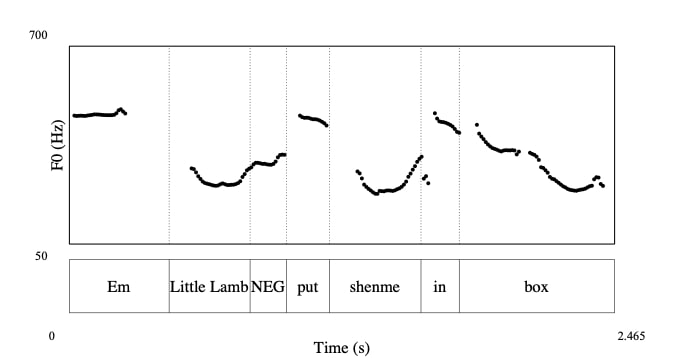
\includegraphics[width=0.6\textwidth]{figures/pitch-FC1wh.jpg}
    \caption{Pitch contour associated with a \twh-interrogative sentence}
    \label{fig:man:wh1}
\end{figure}

\begin{figure}[H]
    \centering
    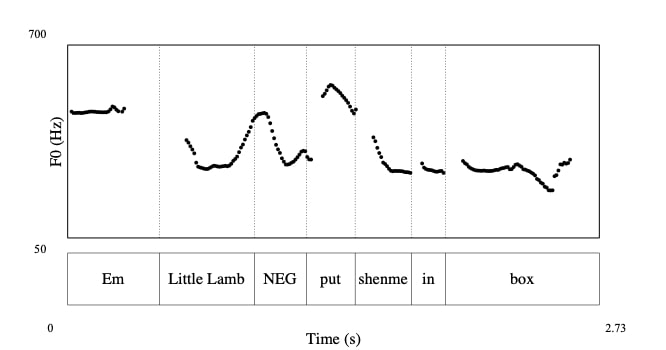
\includegraphics[width=0.6\textwidth]{figures/pitch-FC0wh.jpg}
    \caption{Pitch contour associated with a \twh-indefinite sentence}
    \label{fig:man:wh0}
\end{figure}

 Figure~\ref{fig:man:wh1} shows the pitch contour of the interrogative interpretation of \twh{} and Figure~\ref{fig:man:wh0} shows the indefinite interpretation. The former prosody is associated with [+int] and the latter with [$-$int], and the crucial difference is that the interrogative \tit{shenme} is produced with prosodic prominence (longer duration, extended lexical tone). 

Polar interrogatives in Mandarin also have SVO word order, but are distinguished from declaratives by surface features like the question-forming particle \tit{ma} or the A-not-A construction, as in (\ref{bg-syn:ma}) and (\ref{bg-syn:anota}).

\bex{bg-syn:ma}
\gll Xiaoxiao	chi-le	zaocan		\tun{ma}\\
Xiaoxiao	eat-ASP	breakfast	\Sfp{}\\
``Did Xiaoxiao eat breakfast?''
\eex
\bex{bg-syn:anota}
\gll Xiaoxiao	\tun{chi-mei-chi}	zaocan?\\
	Xiaoxiao	eat-\Neg-eat	breakfast\\
	``Did Xiaoxiao eat breakfast?''
\eex


Sentence final particles (SFPs) like \ma{} are  particles at the right edge of a clause (\citealt{chao1968, zhudexi, huang1982, cheng1991, liboya2006} among others). Many SFPs such as \tit{ba, ya} can occur in any clause type, but \ma{} can only occur in polar interrogatives that do not have the A-not-A form seen in (\ref{bg-syn:anota}). 




To summarize the discussion so far, the surface form of [+int] in Mandarin is sentence final particle \ma{}, A-not-A construction, \twh{} with prominence. 

Imperatives in Mandarin share many of the properties of imperatives in English, namely the lack of subjects. This clause type is sometimes marked by a negative modal \tit{bie} (and its etymologically related modal \tit{beng}), which only occurs in imperatives (\cite{chao1968, lithompson}):

\bex{ex:man:bie}
\bxl{ex:man:bie:imp}
\gll \tbf{Bie} pao!\\
Don't run\\
``Don't run!''
\ex 
\gll *Zhangsan \tbf{bie} pao.\\
Zhangsan don't run\\
(intended) Zhangsan doesn't run.
\exl
\eex 

Using \tit{bie} as a diagnostic for imperatives, we can see that Mandarin [imp] can be embedded (\cite{lithompson, chen2005imp}), and certain verbs like \tit{zhuzhang} selects [imp]:

\bex{ex:man:embed-imp}
\gll Wo \tun{zhuzhang} Lisi \tbf{bie} chu-guo.\\
I advocate Lisi don't exit-country\\
\trans ``I have the opinion that you don't leave the country.'' \hfill \textcite[p.458]{lithompson}
\eex

While some argue that certain \Sfp{s} like \tit{ba} are imperative particles (\cite{zhudexi,chao1968,lithompson}), they can actually appear in declaratives, imperatives, and interrogatives, and do not necessarily convey a request/command force (\cite{YY2021}):
\bex{ex:mancl:ba}
Xiayu le \tbf{ba}?\\
rain \Asp{} \Sfp{}\\
\trans ``It's raining?''
\eex

Similarly, when these particles append to a declarative clause, they do not change the clause type to [+int]:
\bex{ex:mancl:dec-q}
\gll %想 坐 啊 ?	Tong
Xiang zuo a?\\
want sit \Sfp{}\\
``Want to sit on it?''
\hfill Declaratives as question\\
Mother of Tong, Session 01;08;22
\eex

The particle \tit{a} elicits a discourse effect along the lines of ``we both know $p$ (or the answers to the question $q$), but let's put it on the table.'' I do not consider this particle changes the clause to an interrogative, the same way that final rise does not change English declaratives into a different clause type. But the discourse effect of the whole utterance is similar to a question, namely the speaker wants the addressee to respond. 

I therefore do not assume that sentence final particles like \tit{ba} and \tit{a} that can occur across clause types as related to [imp] or [+int].

In sum, [+int] in Mandarin may show up in the surface form of the sentence as the presence of \twh{} with prominence, sentence final \tit{ma}, or A-not-A structure; [imp] shows as sentences without subjects or with second person subjects, and as special negative modal \tit{bie} or \tit{beng} in negative imperatives. 

Mandarin learner also face the same learning problem as English learners: the clause type feature is abstract and is related to a variety of surface forms, none of which is obligatorily present and many of which can occur in sentences with a different clause-type feature on $C^{0}$. For example, even though [imp] is related to null subjects, but since Mandarin is a pro-drop language, observing that a sentence does not have subjects does not necessarily mean that $C^{0}$ is [imp].  


\subsection{Mandarin-acquiring children's knowledge of clause types}
\label{sec:mancl:bg:child}
In this section we will look at evidence for Mandarin-acquiring children's knowledge regarding the features reviewed in the last section. For many of these features, we do not have a lot evidence from the comprehension side, and we have to rely on data from children's production alone to make inferences about their knowledge. As production might not be accurate reflection of children's grammar, we will be conservative in our inference.   

\tsc{\textpm subjects}   As Mandarin do not have subject-verb agreement, and do not have expletive subjects, it is hard to assess chidlren's knowledge regarding subjecthood. But observations of children's production data before 18 months old suggest that they understand the basic word order of Mandarin as SVO (\cite{tardif1993verb,tardif1996verb}). They also produce subject control sentences (e.g. \tit{Zhangsan tried PRO to help me}) correctly before turning 2 (\cite{yang2015control}). While this is out of our interested age range, but studies have demonstrated that 2.6-year-olds can correctly distinguish subjects from topics (\cite{chien1985subj}). 

\tsc{\textpm verbs} By 18 months old, Mandarin-acquiring infants produce many verbs, and use verbs productively in many contexts; while this does not necessarily mean that they have a verb category, it is consistent with the hypothesis that they do (\cite{tardif1993verb,tardif1996verb, xiaolee2006,zhangshili2015infant}, among many others). 13-month-olds also demonstrate the ability to categorize novel words as verbs using frequent frames related to verbs, such as auxiliaries (e.g. \tit{bie} ``don't'') and focus particles (e.g. \tit{ye} ``also'', \cite{zhangshili2015infant}; \cite{ying2021func} for 19-month-olds).

\tsc{\textpm modal auxiliary}  \cite{zhangshili2015infant} find that 12mo use functional words to categorize content words, specifically they could use the negative imperative modal \tit{bie} to identify the follow-up item is a verb, suggesting that children might be sensitive to the presence of these modal auxiliaries.  %Children are found producing modal auxiliaries like \tit{neng} from 18 months old (\cite{}), but it is unclear whether 


\tsc{\textpm \tit{wh}-phrases} Children start producing interrogative \twh{} as early as 14 months old (\cite{lee1989acq, fan2012, linjing2014}); both comprhension experiments and corpus data show that they are also found to answer \tit{where}, \tit{who}, \tit{what} questions appropriately at 18 months old (\citealt{fan2012,moradlou2020}). While we have evidence that 3-year-olds can use prosodic prominence to infer whether the \twh-sentence is [+int] (\cite{WHanything}), we do not have evidence for younger children. In the corpus study, I follow the practice in the last chapter and classify \twh-phrases with focus particles and connectives (e.g. \tit{yaobu} ``if'') as `Unknown Functional Items' (UFI).

\tsc{A-not-A structure} As noted earlier, A-not-A structure and sentence-final \tit{ma} both distinguish interrogatives from declaratives in Mandarin. But while there are evidence suggesting that children start producing negation around 1.5 years old (\cite{lee1982,fan2007,li2019neg, huang2022manchild} among others), we do not have evidence for whether children perceive A-not-A sentences differently from simple negation sentences. Similarly, we do not have evidence for whether children treat \tit{ma} differently from sentences with other sentence final particles like \tit{ya}. I therefore simulated a conservative learner who do not have access to A-not-A and \tit{ma} features, and a knowledgeable learner who have access to these two features. 





\section{Corpus study}
\label{sec:mancl:corpus}

\subsection{Corpus and methods}
\label{sec:mancl:corpus:method}
This study used data from the Tong subcopora (\cite{TongCorpus}) from CHILDES (\cite{CHILDES}), which contains audio and video recordings of weekly hour-long free play sessions between Tong and his caregivers from 1;7-3;4 in Shenzhen, China where Mandarin is the language of the community. Although this corpus only contains data from one child, it is the most comparable to the Providence Corpus in the child’s age range and availability of audio/video data. If more corpora from Mandarin-speaking children become available in the future, the methodology developed here can be applied to them. Another problem with the corpus is that it does not have data from before when the child is 18 months old, which is older than our assumed age that children figure out the clause type categories and older than the children in the English corpus study. However, while the pragmatics of parent-child interaction might change with children's age, the morpho-syntactic properties of parents' sentences should stay constant. Therefore, we assumed that the input sentences share similar properties as parents' sentences before Tong turns 18 months old. Once the corpus releases data from before 18 months old, we would apply the same methodology to these data. 

We sampled 500 conversational turns from each session from when the child was 01;07;18 to 2;2;16. Each session was coded by two annotators independently for the Clause Type and Speech Act information (mean cohen's $\kappa$: 0.8). For the morpho-syntactic features, initial annotation was generated by a script (\textcolor{red}{url}) using the morphological tagging provided by the corpus, and then manually corrected. In total, 4501 utterances were annotated. 

\subsubsection{Clause Type}

Same as the English corpus study reported in the last chapter, each sentence was annotated with their clause type category, \diis{} (\ref{ex:mancl:annt:cl:dec}-\ref{ex:mancl:annt:cl:imp}). Sentences with only one noun phrase or injectives were annotated as ``fragments'':\footnote{Sentences without verbs might not be fragments in Mandarin, as the copula \tit{shi} ``be'' is optional:
\begin{xlist}
\ex 
\gll Zhe wode.\\
This mine.\\
\trans `This is mine.'
\end{xlist}
}

\bex{ex:mancl:annt:cl}
\bxl \label{ex:mancl:annt:cl:dec}
\gll Wazi shi le.\\
Sock wet \Sfp{}\\
``Your socks got wet.'' \hfill Declarative
\ex \label{ex:mancl:annt:cl:int}
\gll Kandao le ma?\\
See \Asp{} \Sfp{}\\
\trans``Do you see it?''  \hfill Interrogative
\ex \label{ex:mancl:annt:cl:imp}
\gll Gei wo hongse de na-ge.\\
Give me red \tsc{poss} that-\Cl{}\\
\trans``Give me the red one.'' \hfill Imperative
\ex \label{ex:mancl:annt:cl:frag}
\gll Ai-ya!\\
\tsc{intj} \\
\trans ``Wow!'' \hfill Fragments
\exl
\eex

The three major speech acts were also annotated, same as English.

\subsubsection{Morpho-syntactic features for clause typing}

As reviewed in the last section, Mandarin-acquiring children at 18 months old can perceive many morpho-syntactic properties related to clause typing in Table~\ref{tab:mancl:grammar}. In particular, they might be able to identify the subject, verb, auxiliary of the sentence, and distinguish functional from lexical items. We additionally adopted the conservative assumption that children at this age might not be able to identify all the \twh-items at this stage,but they might be able to classify them as functional elements, as they may know the distinction between functional and content elements. We therefore put \twh-items, quantifiers, connectives (e.g. \tit{haishi}, the interrogative ``or''), and focus particles in one category ``unknown functional item (UFI),'' and annotated its position in a sentence: sentence initial, sentence-medial but before the verb, after the verb, or sentence final. In addition to these surface features that were also annotated in the English corpus study, we also annotated for whether the sentence contains an A-not-A structure, and whether there is a sentence-final \tit{ma} particle. But since we do not have evidence for whether children around 18 months can perceive these two cues, as discussed in the last section, when simulating children's learning process, we will compare conservative models without these two cues, and knowledgeable models with these two cues.


Each sentence was annotated with whether or not a surface feature is present. (\ref{ex:mancl:schema:formal:verb})-(\ref{ex:mancl:schema:formal:ma}) demonstrate the surface features we annotated and their examples.  


\begin{exe} \label{ex:mancl:schema:formal:verb}
\ex 
\gll \tbf{kan} zhe-ge.\\
Look this-\Cl{}\\
\trans `Look at this one!'' \hfill +Verb
\end{exe}

\bex{mancl:schema:formal:subj}
\gll \tbf{Wo} zhidao.\\
I know\\
\trans ``I know.'' \hfill +Subject
\eex

\begin{comment}
\bex{mancl:schema:formal:asp}
\bxl
\gll Mama mei gei ni mai \tbf{guo} zhege wanju\\
Mom \Neg{} to you buy \Asp{} this toy\\
\trans`` Mom never bought this toy for you.'' \hfill +Aspect
\exl
\eex
\end{comment}

\bex{mancl:schema:formal:aux}
\bxl
\gll Xiaopengyou bu-\tbf{neng} peng.\\
Children \Neg-can touch\\
\trans ``Children can't touch (this).'' \hfill +Auxiliary
\exl
\eex

\bex{mancl:schema:formal:ufi}
+ Unknown functional items:
\bxl
\gll \tbf{Yaobu} na zhe-ge kapian lai jiao ba\\
%要 不 拿 这 个 卡片 来 教 吧 .
What-if take this-\Cl{} card to teach \Sfp{}\\
\trans ``What if (you) teach with this card.''  \hfill Sentence-initial UFI

\ex
\gll Zheli \tbf{hai} you labi.\\
Here also have crayon\\
\trans ``There's also crayons." \hfill Pre-verbal UFI
\ex
\gll  Limian you \tbf{shenme} ya?\\
Inside have what \Sfp{}\\
\trans ``What's inside?" \hfill Post-verbal UFI
\ex 
\gll Guolai \tbf{ba}\\
Come \Sfp{}\\
\trans ``Come here!'' \hfill Sentence final particle
\exl
\eex

\bex{mancl:schema:formal:anota}
+ A-not-A: 
\bxl
\gll Jintian \tbf{leng-bu-leng} a?\\
Today cold-\Neg-cold \Sfp{}\\
\trans ``Is it cold today?" \hfill \tit{Adj-not-Adj}
\ex 
\gll Ni \tbf{hui-bu-hui} xiezi?\\
You can-\Neg-can write\\
\trans ``Can you write? \hfill \tit{Aux-not-Aux}
\ex \gll Ni \tbf{you-mei-you} xiaoqiche?\\
You have-\Neg-have car\\
\trans ``Do you have cars?'' \hfill \tit{V-not-V}
\ex 
\gll \tbf{Chuan-hao} yifu \tbf{meiyou}?\\
Put-well cloth \Neg{}\\
\trans ``Did you put on your coat?'' \hfill \tit{A-not}
\exl
\eex

\bex{ex:mancl:schema:formal:ma}
\gll Xiayu le \tbf{ma}?\\
Rain \Asp{} \tsc{ma}\\
\trans ``Is it raining?'' \hfill +\tit{ma}
\eex

\subsection{Results}
\label{sec:mancl:corpus:results}

\subsubsection{Overview}
\label{sec:mancl:corpus:results:mapping}

In total, 3077 utterances were annotated. Figure~\ref{fig:man-real-cldist} shows the distribution of clause types in the dataset. Same as results in the English dataset, Declarative clauses are the most frequent clause type, followed by interrogatives and imperatives. 

\begin{figure}[H]
    \centering
    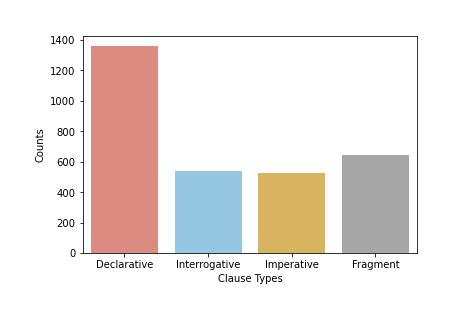
\includegraphics[width=0.7\textwidth]{figures/man-real-cldist.jpg}
    \caption{Distribution of clause types in the corpus}
    \label{fig:man:real-cldist}
\end{figure}

Within interrogatives (Figure~\ref{fig:man:real-subint}), \twh-interrogatives (\ref{ex:man:int:wh}) are more frequent than other types of interrogatives, a pattern similar to English; followed by A-not-A (\ref{ex:man:int:anota}) and \tit{ma}-interrogatives (\ref{ex:man:int:ma}). Disjunctive interrogatives with \tit{haishi} ``or'' (\ref{ex:man:int:haishi}) are relatively rare. 
\begin{figure}[H]
    \centering
    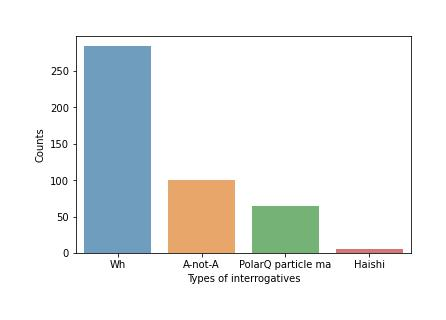
\includegraphics[width=0.7\textwidth]{figures/man-real-subint.jpg}
    \caption{Subcategories of interrogatives}
    \label{fig:man:real-subint}
\end{figure}

\bex{ex:man:int:corpus}
\bxl\label{ex:man:int:wh}
\gll Zhe \tbf{shenme} a?\\
this what \Sfp{}\\
``What is this?'' \hfill  \twh-interrogative\\Mother of Tong, Session 01;10;17
\ex\label{ex:man:int:anota}
\gll Na \tbf{xi-bu-xihuan} he naifen a?\\
Then like-\Neg-like drink {baby formula} \Sfp{}\\
\trans ``Do you like {baby formula} then?'' \hfill A-not-A interrogative\\
Mother of Tong, Session 02;00;19
\ex\label{ex:man:int:ma}
\gll Ni Zhidao \tbf{ma}?\\
You know \tsc{ma}\\
\trans ``Do you know?'' \hfill Ma-interrogative\\Mother of Tong, Session 01;10;17
\ex\label{ex:man:int:haishi}
\gll Qiezi haochi \tbf{haishi} baicai haochi?\\
Eggplant tasty or cabbage tasty\\
\trans ``Is eggplant tastier or cabbage tastier?"\hfill \tit{Haishi} interrogative\\Father of Tong, Session 01;08;22
%茄子 好吃 还 是 白菜 好吃 ? 
\exl
\eex

\begin{figure}[H]
    \centering
    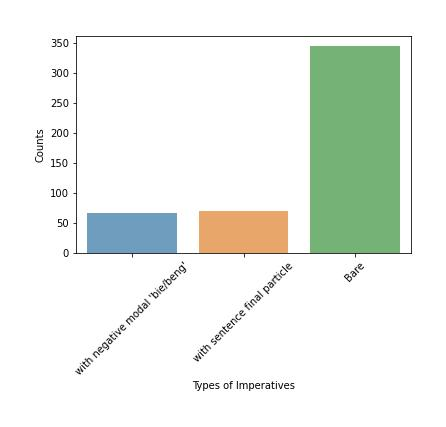
\includegraphics[width=0.7\textwidth]{figures/man-real-subimp.jpg}
    \caption{Subcategories of imperatives}
    \label{fig:man:real-subimp}
\end{figure}

Imperatives (Figure~\ref{fig:man:real-subimp}) sentences mostly come without any marker like (\ref{ex:man:impbare}); \tit{bie}-imperatives (\ref{ex:man:impbie}) and SFP-imperatives (\ref{ex:man:impba}) are equally frequent. 


\bex{ex:man:imp:corpus}
\bxl\label{ex:man:impbare}
\gll Kan zhege shi shenme dongxi\\
look this is what thing\\
``See what this is!''  \hfill Imperative (used as a question)\\
Mother of Tong, Session 02;00;19

\ex \label{ex:man:impbie}
\gll \tbf{Bie} fan le!\\
Don't turn \Asp{}\\
``Stop messing around!'' \hfill \tit{Bie}-imperative\\Mother of Tong, Session 02;00;09
\ex \label{ex:man:impba}
\gll Reng zheli \tbf{ba}\\
throw here \Sfp{}\\
\trans ``Throw it here!''
\hfill SFP imperative\\Mother of Tong, Session 02;01;17
\exl
\eex


As for speech acts, Figure~\ref{fig:man-real-sp} shows the distribution of speech acts. Same as English, assertions are the most frequent speech acts, followed by questions and requests. 
\begin{figure}[H]
    \centering
    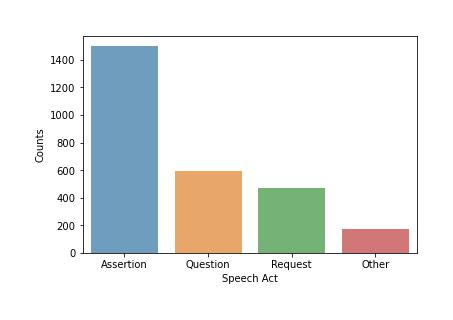
\includegraphics[width=0.7\textwidth]{figures/man-real-sp.jpg}
    \caption{Distribution of speech acts in the corpus}
    \label{fig:man-real-sp}
\end{figure}

The mapping between speech acts and clause types also shows a similar pattern as English, as illustrated by Figure~\ref{fig:man-real-clsp} and \ref{fig:man-real-spcl}. Declaratives are mostly used as assertions, interrogatives as questions, and imperatives as requests. 

\begin{figure}[H]
    \centering
    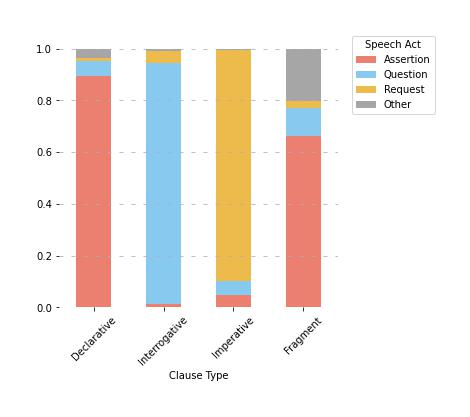
\includegraphics[width=0.7\textwidth]{figures/man-real-clsp.jpg}
    \caption{The speech acts performed by each clause type in parents' speech}
    \label{fig:man-real-clsp}
\end{figure}

\begin{figure}[H]
    \centering
    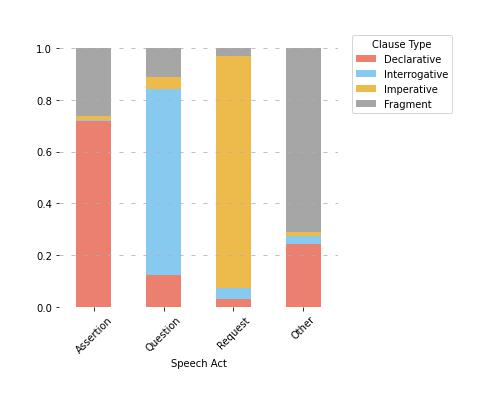
\includegraphics[width=0.7\textwidth]{figures/man-real-spcl.jpg}
    \caption{The clause type used to express each speech act in parents' speech}
    \label{fig:man-real-spcl}
\end{figure}

The proportion of mismatches are small, and they form a systematic subcategory. All interrogatives are used as assertions are rhetorical questions (\ref{ex:mancl:int-asst}). The proportion of interrogatives as requests is smaller than in English (\ref{ex:mancl:int-req}). Even in the small portion of cases, it could be debated whether the non-literal speech act of this sentence is request, as the mother is still asking about the child's ability whereas indirect requests in English like \tit{can you pass the salt} are much less saliently about the addressee's ability. 

\bex{ex:mancl:int-asst}
\gll Ni xia gaoxing ge shenme ya\\
you blindly happy \Cl{} what \Sfp{}\\
``What are you happy about.'' \hfill Interrogative as question \\
Mother of Tong, Session 02;00;19
%你 瞎 高兴 个 什么 呀 
\eex

\bex{ex:mancl:int-req}
\gll Tongtong hui bei ma?\\
Tongtong can recite \tsc{ma}\\
\trans ``Can you recite (this poem), Tongtong?''
\hfill Interrogative as Requests \\
Mother of Tong, Session 02;00;19
%你 瞎 高兴 个 什么 呀 
\eex

When imperatives are not used as requests, it is almost exclusively with \tit{kan} ``look" and \tit{gaozu} ``tell'':
\bex{ex:mancl:imp-q}
\gll Gaosu mama zhe shi shenme ya?\\
Tell mom this is what \Sfp{}\\
``Tell mom what this is'' \hfill Imperative as question\\
Mother of Tong, Session 02;00;19
\eex

Declaratives as questions often occur with sentence final particles like \tit{a}:
\bex{ex:mancl:dec-q}
\gll %想 坐 啊 ?	Tong
Xiang zuo a?\\
want sit \Sfp{}\\
``Want to sit on it?''
\hfill Declaratives as question\\
Mother of Tong, Session 01;08;22
\eex

As we have discussed, \tit{a} does not change the clause category of the sentence, but still elicits a discourse effect similar to questions' effect, namely the speaker wants the addressee to settle an issue.
%The particle \tit{a} elicits a discourse effect along the lines of ``we both know $p$ (or the answers to the question $q$), but let's put it on the table.'' I do not consider this particle changes the clause to an interrogative, the same way that final rise does not change English declaratives into a different clause type. But the discourse effect of the whole utterance is similar to a question, namely the speaker wants the addressee to respond. 


\subsubsection{Morpho-syntactic cues}
\label{sec:mancl:corpus:results:syn}


\begin{figure}[H]
    \centering
    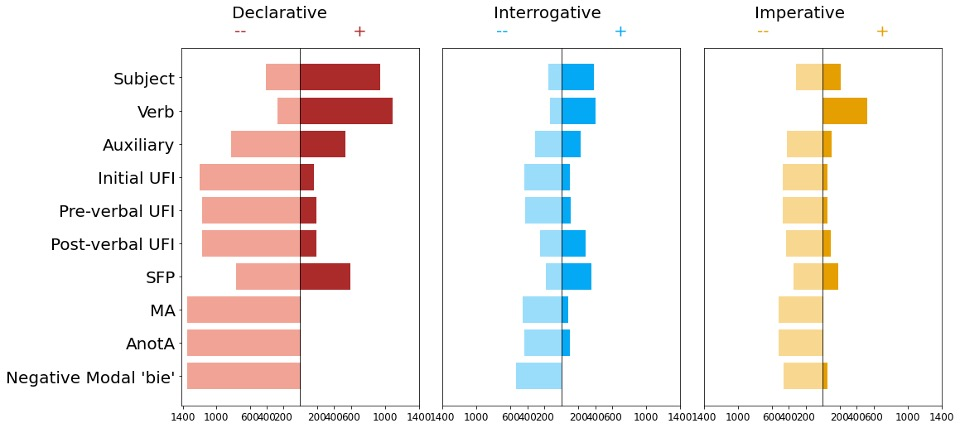
\includegraphics[width=1\textwidth]{figures/man-real-syncluster.jpg}
    \caption{Number of sentences with/without various formal cues in each clause type; darker colors represent number of sentences with the cue, lighter colors, number of sentences without the cue }
    \label{fig:man-real-syncluster}
\end{figure}


%\subsubsection{Informativeness of the cues}
%\label{sec:mancl:corpus:results:supervised}


\section{Modeling the learning of clause type in 
Mandarin}
\label{sec:mancl:model}


\subsection{Performance of the \dlearnerabbr{} model}
\label{sec:mancl:model:results:d}

Figure~\ref{fig:man-baseline-heatmap} shows the proportion of \diis{} in each identified cluster, and Figure~\ref{fig:man-baseline-heatrev} shows the proportion of sentences clustered together. In other words, Figure~\ref{fig:man-baseline-heatmap} shows whether each cluster mostly consists of one clause type, and Figure~\ref{fig:man-baseline-heatrev} shows whether each clause type is put in one cluster.  



\begin{figure}[H]
    \centering
    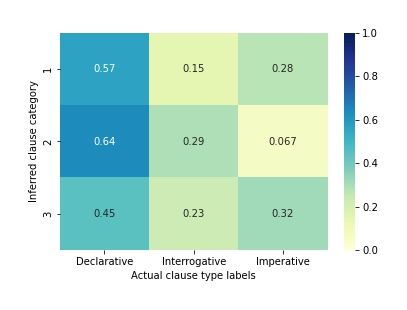
\includegraphics[width=0.7\textwidth]{figures/man-baseline-conservative-heat.jpg}
    \caption{The proportion of \diis{} in each of the three clusters identified by the \dlearnerabbr{} model}
    \label{fig:man-baseline-conservative-heat}
\end{figure}


\begin{figure}[H]
    \centering
    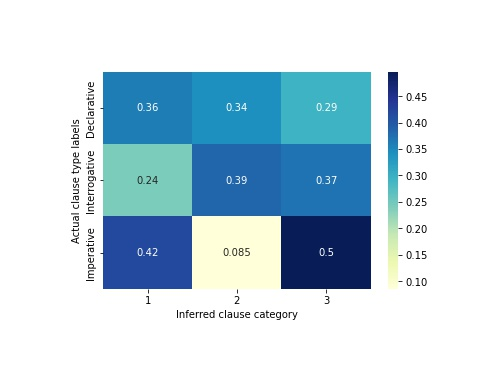
\includegraphics[width=0.7\textwidth]{figures/man-baseline-conservative-heatrev.jpg}
    \caption{The proportion of actual \diis{} clustered in one category}
    \label{fig:man-baseline-conservative-heatrev}
\end{figure}

\begin{figure}[H]
    \centering
    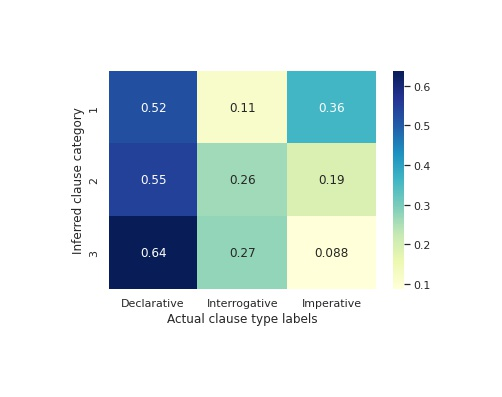
\includegraphics[width=0.7\textwidth]{figures/man-baseline-mid-heat.jpg}
    \caption{The proportion of \diis{} in each of the three clusters identified by the \dlearnerabbr{} model}
    \label{fig:man-baseline-mid-heat}
\end{figure}


\begin{figure}[H]
    \centering
    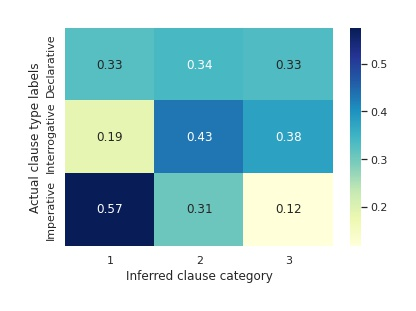
\includegraphics[width=0.7\textwidth]{figures/man-baseline-mid-heatrev.jpg}
    \caption{The proportion of actual \diis{} clustered in one category}
    \label{fig:man-baseline-mid-heatrev}
\end{figure}

Overall, Figure~\ref{fig:man-baseline-heatmap} shows that the \dlearnerabbr{} model identifies an interrogative cluster and a declarative cluster. Cluster~$0$ mostly contains interrogative clauses, as 90\% of sentences in this cluster are interrogative; Cluster~$2$ is mostly declarative, and 86\% of the data in this cluster are declaratives. Cluster~$1$ is split between declaratives and imperatives. Figure~\ref{fig:baseline-heatrev} shows that 87\% of interrogatives and 93\% of imperatives are clustered together in Cluster~$0$ and $1$ respectively. While most of declaratives are classified in Cluster~$2$, a proportion is classified in Cluster~$1$.

These results seem to suggest that the \dlearnerabbr{} found two out of three clause types, but how do these clause types look like? Did the model find the right morpho-syntactic properties to associate with each clause type? Figure~\ref{fig:baseline-syncluster} plots the morpho-syntactic profile of each cluster identified by the \dlearnerabbr{}. Darker colors represent sentences with the morpho-syntactic property, and lighter colors represent sentences without the property. 

\begin{figure}[H]
    \centering
    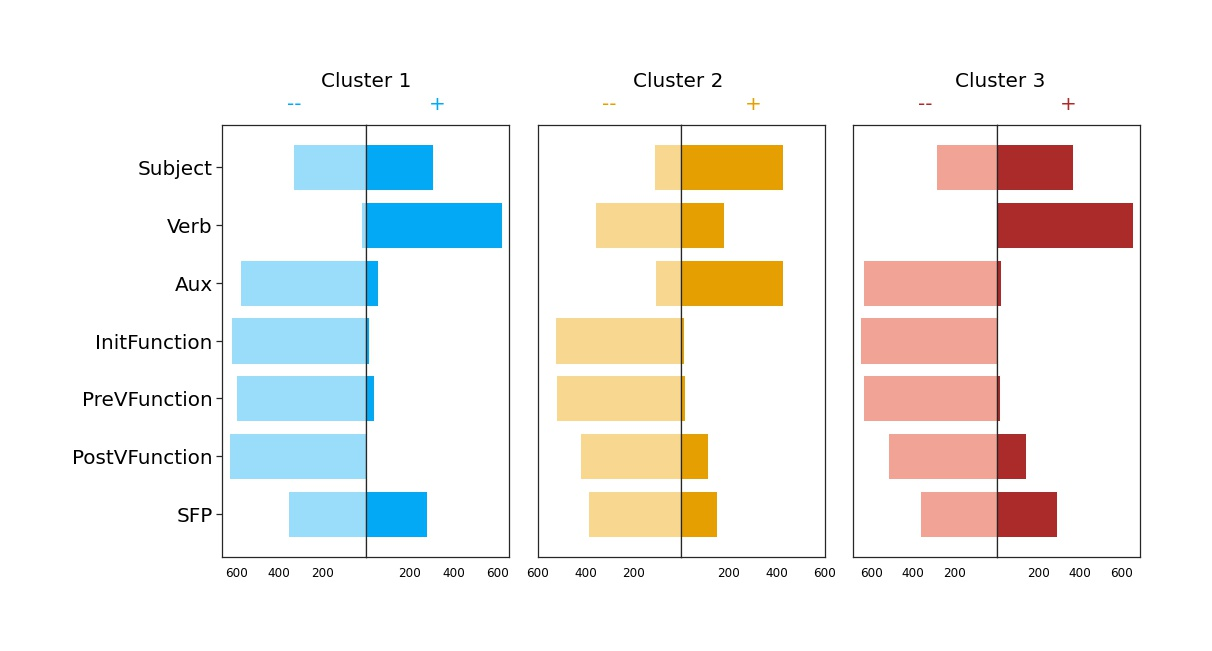
\includegraphics[width=1\textwidth]{figures/man-baseline-conservative-syncluster.jpg}
    \caption{The number of sentences with/without certain formal features in each cluster (Cluster 0 $\sim$ Interrogatives, Cluster 1 $\sim$ Imperatives, Cluster 2 $\sim$ Declaratives), darker colors represent the number of sentences with the feature. UFI stands for Unknown Functional Item (e.g. \twh{}), see Table~\ref{tab:mancl:formal-schema} for details.}
    \label{fig:man-baseline-syncluster}
\end{figure}

We can see that Cluster~$0$, which is 90\% interrogative clauses, is associated with [+int] morpho-syntactic properties such as subject-auxiliary inversion and sentence-initial unknown functional item (e.g. \twh{}).

\subsection{Performance of the \plearnerabbr{} model}
\label{sec:mancl:model:results:d}

Figure~\ref{fig:man-target-heatmap} shows the proportion of \diis{} in each identified cluster, and Figure~\ref{fig:man-target-heatrev} shows the proportion of sentences clustered together. 
\begin{figure}[H]
    \centering
    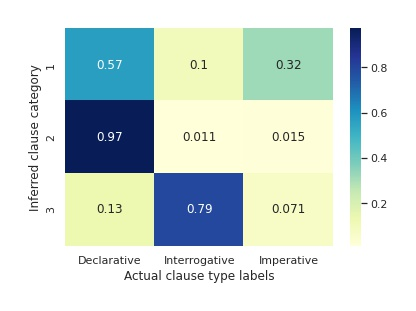
\includegraphics[width=0.7\textwidth]{figures/man-target-conservative-heatmap.jpg}
    \caption{The proportion of \diis{} in each of the three clusters identified by the \plearnerabbr{} model}
    \label{fig:man-target-conservative-heatmap}
\end{figure}




\begin{figure}[H]
    \centering
    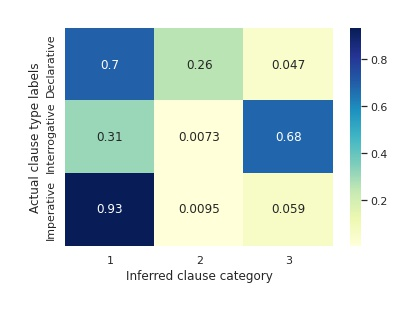
\includegraphics[width=0.7\textwidth]{figures/man-target-conservative-heatrev.jpg}
    \caption{The proportion of actual \diis{} clustered in one category}
    \label{fig:man-target-conservative-heatrev}
\end{figure}
%Rand comparison

%confusion matrix

We can see that the \plearnerabbr{} model clearly identifies a declarative, an interrogative, and an imperative cluster: 94\% of Cluster~$0$ are interrogatives, 86\% of Cluster~$1$ are declaratives, and 70\% of Cluster~$2$ are imperatives. The three clause types in English are also mostly clustered together by the model: 95\% of declaratives, 90\% of interrogatives, and 87\% of imperatives are clustered together in Cluster~$1$, $0$, $2$ respectively. Compare to \dlearnerabbr{}, this learner is able to find the right clause types in English.


Figure~\ref{fig:man-target-syncluster} shows the morpho-syntactic profile of each cluster identified by the \plearnerabbr{}. 

\begin{figure}[H]
    \centering
    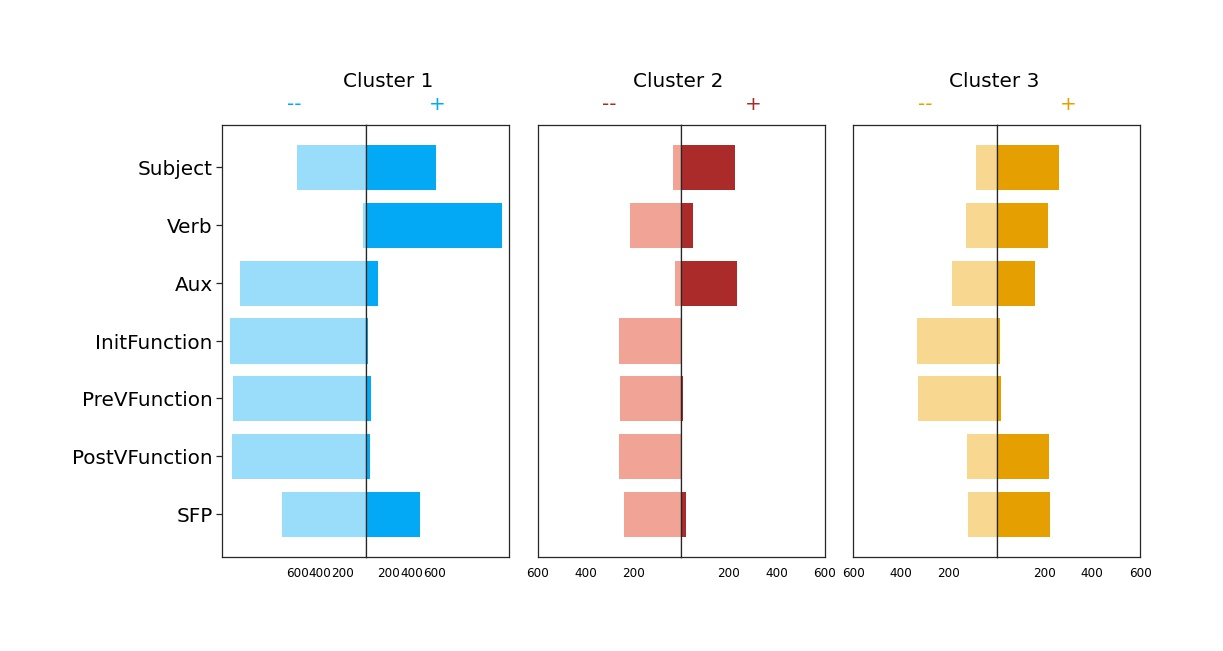
\includegraphics[width=1\textwidth]{figures/man-target-conservative-syncluster.jpg}
    \caption{The number of sentences with/without a formal property in each cluster (Cluster 0 $\sim$ Interrogatives, Cluster 1 $\sim$ Declaratives, Cluster 2 $\sim$ Imperatives), darker colors represent the number of sentences with the property, lighter colors represent sentences without the property.}
    \label{fig:man-target-conservative-syncluster}
\end{figure}

The profile of the three clusters resembles the profile of \diis{} in our corpus study (Figure~\ref{fig:man-real-syncluster}). The cluster for interrogatives has more sentences with subject-auxiliary inversion and clause-initial unknown functional items (e.g. \twh{}), and the cluster for imperatives is characterized by the lack of subjects and verb suffixes. 

\subsection{Simulations with noisy pragmatic information}
\label{sec:mancl:model:results:noisy}

Figure~\ref{fig:noisy-rand-compare} shows the simulations with 0-100\% noise. The performance of the \dlearnerabbr{} model in our last simulation is marked by the dotted line. As can be seen, the \plearnerabbr{} learner outperforms the \dlearnerabbr{} learner up until there is around 80\% of noise in speech act, and even at 80\% level there are iterations that outperforms the \dlearnerabbr{}. This suggests that a little pragmatics goes a long way, as the learners with noisy pragmatic information still outperforms the one without. 

\begin{figure}[H]
    \centering
    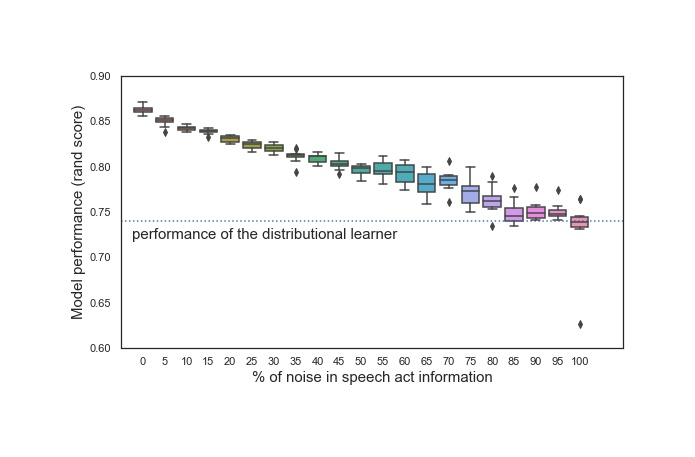
\includegraphics[width=1\textwidth]{figures/noisy-rand-compare.jpg}
    \caption{Performance of the \plearnerabbr{} model with different levels of noise in the speech act information; dotted marks the rand score of the \dlearnerabbr{} learner}
    \label{fig:man-noisy-rand-compare}
\end{figure}


Looking at the learner at maximum noise level, we can see that the \plearnerabbr{} reverts back to the performance of the \dlearnerabbr{} fails to identify a cluster for declaratives (Figutre~\ref{fig:noisy100-heatmap}. Similar to the distributional learner, the cluster for imperatives also have declaratives (\ref{fig:noisy100-heatrev}). 



\begin{figure}[H]
    \centering
    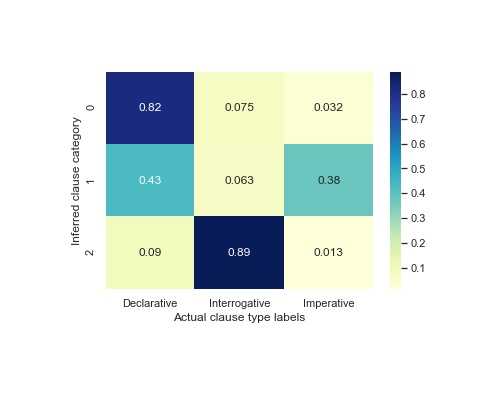
\includegraphics[width=0.7\textwidth]{figures/noisy100-heatmap.jpg}
    \caption{The proportion of \diis{} in each of the three clusters (100\% noise in speech act information) }
    \label{fig:noisy100-heatmap}
\end{figure}

\begin{figure}[H]
    \centering
    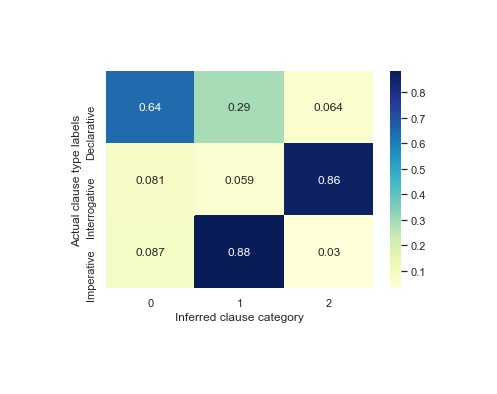
\includegraphics[width=0.7\textwidth]{figures/noisy100-heatrev.jpg}
    \caption{The proportion of actual \diis{} clustered in one category}
    \label{fig:noisy100-heatrev}
\end{figure}

Looking at the morpho-syntactic profile of this model with random speech act information behaves like the \dlearnerabbr{} model, and fails to identify the properties of English imperatives and declaratives.

\begin{figure}[H]
    \centering
    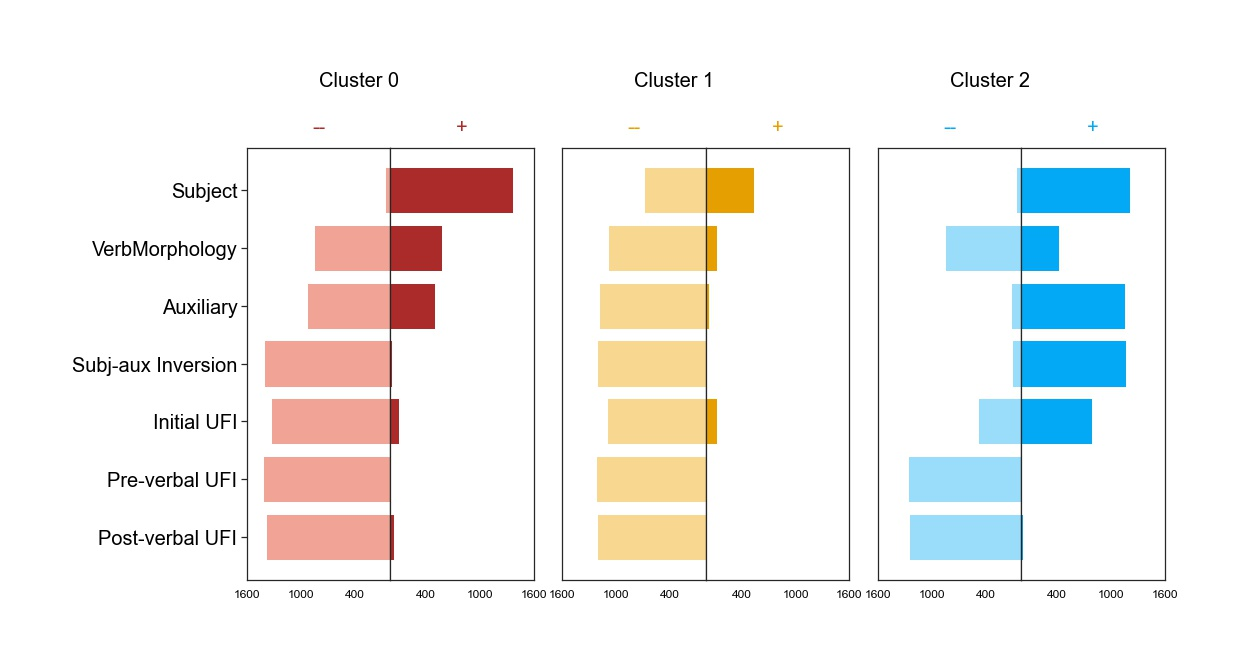
\includegraphics[width=1\textwidth]{figures/noisy100-syncluster.jpg}
    \caption{The number of sentences with/without certain formal features in each cluster (Cluster 0 $\sim$ Interrogatives, Cluster 1 $\sim$ Imperatives, Cluster 2 $\sim$ Declaratives), darker colors represent the number of sentences with the feature.}
    \label{fig:noisy100-syncluster}
\end{figure}


\section{Discussion}
\label{sec:mancl:discussion}

This chapter investigates how Mandarin-acquiring 18-month-olds learn to identify the three clause types. As [+int] and [imp] in English and Mandarin are related to different surface features, comparing these two languages provide us with an opportunity to see the role of pragmatics in different languages.

Same as English parents, Mandarin parents also 
use clause types systematically, and the three clause types are predominantly mapped to their canonical functions (declaratives to assertions, interrogatives to questions, imperatives to requests/commands). The three clause types show different formal profiles in the input: compared to declaratives, interrogatives are more likely to have post-verbal UFIs, and more likely to have A-not-A and sentence final \tit{ma}; imperatives are more likely to not have subjects and negative modal \tit{bie}.

I then investigated the extent to which Mandarin learners need to rely on pragmatic information to identify clause types. I showed that \dlearnerabbr{} simply cannot identify any of the right categories, even when we loosen our assumptions on learners' morpho-syntactic knowledge. But the \plearnerabbr{}, with pragmatic information, could identify all three clause types. Whereas a little pragmatics helps a lot for English learners, Mandarin learners require more accurate pragmatic information to succeed; when the noise in speech act exceeds 40 \% (20\% for learners with less morpho-syntactic knowledge), performance drops to the same level as syntax-only models.

In summary, pragmatics is essential for both English and Mandarin learners. But pragmatics is even more crucial for Mandarin learners, as the morpho-syntactic information is not enough for clause typing. 

So far, we have been assuming that children have access to the speech act information. As we have discussed, this could lead to a chicken-and-egg problem: children need speech act to learn clause type, but at the same time they need clause type to learn speech act. In the next chapter, we explore other cues for speech act that are not clause type-related. As we have demonstrated with our simulations, English learners can tolerate some noise in speech act information. If cues other than clause type (e.g. parents' attention behavior) are informative of speech act to some extent, it might already be sufficient for solving the clustering problem of clause typing. In the next chapter, we specifically look at three such cues, prosody, speech gap, and parents' attention.



\chapter{Prosody }
\label{chap:prosody}



\section{Background}
\label{sec:prosody:bg}
\subsection{Prosody, clause types, and speech acts in English}
In English, whether prosody is a surface feature for clause typing or simply an indicator for questioning is debated. English declaratives tend to be associated with falling intonation, polar interrogatives tend to bear rising intonation, while \twh-interrogatives also generally bear a falling contour (\citealt{ladd1981, ladd2008intonational, hedberg2004wh, hedberg2014corpus} among many others). When declaratives are associated with a  L* H-H\% rising intonation, they tend to be interpreted as questions (i.e. rising declaratives, \citealt{ladd1981,gunlogson2004,gunlogson2008,jeong2018,rudin2018,goodhue2021rd}). The main point of contention comes down to whether sentences like (\ref{ex:bg:theory:prosody:rd}) are declaratives or not (I will use $\nearrow$ to indicate the sentence has a final rising intonation, and $\searrow$ for final fall):
 
\bex{ex:bg:theory:prosody:rd}
It's raining $\nearrow$
\eex
\bex{ex:bg:theory:prosody:fd}
It's raining $\searrow$
\eex


In Gunlogson's \cite*{gunlogson2008} analysis, sentences like (\ref{ex:bg:theory:prosody:rd}) are declarative clauses with a rising intonation, implying that intonation does not affect the clause type feature of the sentence. Meaning-wise, clause type and intonation contribute compositionally to the discourse function of the utterance. 


Many analyses of rising declaratives in the dynamic discourse tradition adopt the same assumption. As these cases are rarely discussed in syntactic literature, it is unclear whether syntacticians would classify them as having [$-$int] or [$+$int]. But we can go through
%the arguments given to other
some typical syntactic tests for
[$+$int], to see if it's possible to assign [$+$int] to
%the sentence
rising declaratives. One test is whether rogative verbs that only select interrogative clauses would embed (\ref{ex:bg:theory:prosody:rd}). If (\ref{ex:bg:theory:prosody:rd}) bears [+int], then the sentence with (\ref{ex:bg:theory:prosody:rd}) embedded under \tit{wonder} should be grammatical.

\bex{ex:bg:theory:prosody:rd-wonder}
*Mary wonders \tun{it's raining}.
\eex

As shown in (\ref{ex:bg:theory:prosody:rd-wonder}), this prediction is not borne out; (\ref{ex:bg:theory:prosody:rd}) cannot be embedded under rogative verbs like \tit{wonder}. This suggests that (\ref{ex:bg:theory:prosody:rd}) does not have the feature [+int]. But it could be that (\ref{ex:bg:theory:prosody:rd}) has a silent [+int], but this silent [+int] is realized as \tit{whether} in embedded context. So instead of (\ref{ex:bg:theory:prosody:rd-wonder}), embedded (\ref{ex:bg:theory:prosody:rd}) should be:

\bex{ex:bg:theory:prosody:rd-whether}
Mary wonders \tun{whether it's raining}.
\eex

As the rising intonation associated with (\ref{ex:bg:theory:prosody:rd}) would not manifest in embedded clauses, it's hard to distinguish the two possibilities syntactically. But \textcite{farkasroelofsen2017} observe that if the embedded clause is preposed, the intonation difference is preserved, and rising declaratives pattern with polar interrogatives in these cases:

\bex{ex:bg:theory:prosody:rd-prepose}
\bxl{}
`It's raining$\searrow$,' it appears/*she wondered.
\ex`Is it raining?,' *it appears/she wondered.
\ex`It's raining$\nearrow$,' *it appears/she wondered.
\exl
\eex

\textcite{farkasroelofsen2017} use this evidence to argue that rising declaratives are similar to interrogatives and that this similarity should be captured in part by syntax. They propose that the syntactic representation of sentence forms have two kinds of clause type markers, \tsc{closed/open} and \tsc{dec/int}, as in (\ref{fig:bg:fb2017}). Although they didn't specify where these markers reside in the syntactic structure, but they seem to adopt a split-CP approach following \textcite{rizzi1997}, and thus the two clause markers are both part of CP. 


\begin{figure}[H]
\begin{center}
\begin{tikzpicture}[level distance=30pt]
\tikzset{level 1/.style={sibling distance=15pt}}
\tikzset{level 2/.style={sibling distance=35pt}}
\Tree
[. CP 
	[. \tsc{open/closed} ]
	[. \tsc{}
		[. \tsc{decl/int} ]
		[. TP \edge[roof]; { } ] 
	]
]
\end{tikzpicture}
\end{center}
\caption{Extended structure of CP proposed by \textcite{farkasroelofsen2017}}
\label{fig:bg:fb2017}
\end{figure}

While the morpho-syntax of a sentence is linked to \tsc{dec/int}, the intonation (rise vs. fall) signals whether C bears the feature [\tsc{open}] or [\tsc{closed}]. Rising declaratives like (\ref{ex:bg:theory:prosody:rd}) would be an ``open declarative,'' with the following structure:

\begin{figure}[H]
\begin{center}
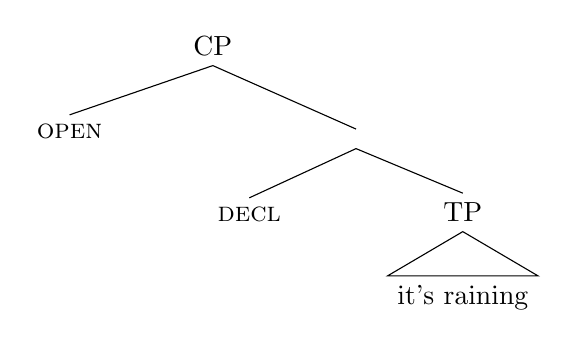
\begin{tikzpicture}
\tikzset{level 1/.style={sibling distance=35pt}}
\tikzset{level 2/.style={sibling distance=35pt}}
\Tree
[. CP 
	[. \tsc{open} ]
	[. \tsc{}
		[. \tsc{decl} ]
		[. TP \edge[roof]; {it's raining} ] 
	]
]
\end{tikzpicture}
\end{center}
\caption{The structure of rising declaratives, adapted from \textcite{farkasroelofsen2017}}
\label{fig:bg:fb2017rd}
\end{figure}

So for \textcite{farkasroelofsen2017}, the clause type category of rising declaratives is not exactly declarative with [$-$int] (but rather [\tsc{open,dec}]), and its semantics is similar to that of the polar interrogatives. 

However, as many have noted, there might be two types of rising declaratives. The one discussed in \textcite{farkasroelofsen2017} is the inquisitive one, but there might an assertive one (\cite{jeong2018, goodhue2021rd}), as shown in (\ref{ex:engcl:annt:rd:a}):

\bex{ex:engcl:annt:rd-cont}
\bxl
\label{ex:engcl:annt:rd:q}
\tit{S and A are on their way to a birthday party for the daughter of A’s friend. They stop at a store to get a birthday card. As they are both scanning the display for a card for the correct age, S is trying to remember how old the girl has just turned, and he thinks he remembers A telling him that she just turned nine, but he wants to confirm it.}\\
\tbf{S: She’s nine$\nearrow$}
\ex
\label{ex:engcl:annt:rd:a}
\tit{S is enrolling his daughter in a summer camp program with the camp organizer A.}\\
S: I want to sign her up for Spanish classes in the mornings, and rock climbing in the afternoons.\\
A: Okay, there are limited places in each activity based on age group, and some of the age groups have already filled up for rock climbing. How old is your daughter?\\
\tbf{S: She’s nine$\nearrow$}
\exl
\hspace*{\fill}\hfill ex. (12-13), \cite[955]{goodhue2021rd}
\eex

In (\ref{ex:engcl:annt:rd:q}), the speaker uses the utterance to elicit a confirmation from the addressee regarding the age of the birthday girl, so the main goal is to solicit responses, similar to that of questions. But in (\ref{ex:engcl:annt:rd:a}), the speaker uses the rising declarative to answer the question raised by the addressee, proposing to add the proposition \tit{she's nine} to the common ground of the conversation. Even though there is an additional effect associated with the utterance (something to the effect of ``Is there still room in the 9-year-old’s rock climbing group?''), this additional effect is not the main goal of the utterance.\footnote{There is another incredulous use of rising declarative, but the two uses mentioned here are more relevant for the current discussion on the speech act of rising declaratives, as most agree that incredulous rising declarative is also ``inquisitive'', same as (\ref{ex:engcl:annt:rd:q}).} Thus, we might not need to assume an interrogative semantics for rising declaratives.\footnote{Note that if we paraphrase (\ref{ex:engcl:annt:rd:a}), we cannot use \tit{wonder} either:

\begin{xlisti}
\ex \label{ex:bg:theory:prosody:rd-prepose2}
\tit{S is looking a flyer looking for Spanish speakers.}\\
``I speak Ladino $\nearrow$," S thinks/$^{??}$ S wonders.
\end{xlisti}

This suggests that the conclusion drawn from the test with pre-posed embedded clause might need to be re-examined.}  As \textcite{goodhue2021rd} demonstrates, it is possible to give a unified account for these two uses of rising declaratives without assuming a separate layer of clause type markers. Therefore, in this dissertation, I assume that rising declaratives are declaratives with [$-$int] in $C^{0}$. Since nobody has argued that interrogatives with falling intonation should be classified as having a different clause type as interrogatives with rising intonation, I assume that intonation can modify the conventional effects of a clause (and hence the speech act expressed), and maybe even serve as a cue for identifying clause types, but [\textpm int] does not manipulate intonation the same way it manipulates, say, the word order of subject and auxiliary.


\subsection{Children's knowledge of prosodic features}
As we have seen in Chapter~\ref{chap:background}, rising intonation tends to associate with interrogatives (particularly polar interrogatives) and questions cross-linguistically. Results from previous experimental and corpus studies suggest that children might be sensitive to the distinction between a final rise (specifically polar interrogative rise) and a final fall. 

From as early as 6 months old, infants are able to identify utterance boundaries, and are sensitive to the edge prosody (\cite{johnson2014edge}). They also can use distinctions in prosodic contours (e.g. final rise vs. fall) to distinguish clause types (polar interrogative vs. declaratives). For example, \textcite{frota2014}) show that as young as 6 months old, European Portuguese-acquiring infants are sensitive to the prosodic distinction between polar interrogatives and declaratives, where prosody is the only cue that distinguishes these two clause types in the language. \textcite{geffenmintz2011} find that when given a combination of word order and prosodic cues, English-acquiring 7-month-olds can distinguish polar interrogatives from declarative assertions. \textcite{soderstrom2005clause} test English-speaking infants between 4.5 months and 2 years old (average 14 months old), and find that they are sensitive to the distinction between declaratives with a falling a rising contour. Before 18 months old, infants acquiring non-lexical tone languages such as English are shown to be sensitive to some tonal distinctions in lexical tone languages such as Mandarin. They are particularly sensitive to the distinction between the rising tone that is similar to English polar-interrogative rise, and the falling tone similar to English declarative fall (\cite{shi2017tone, Hay2019}).%, although it is unclear whether we can draw any conclusions about their sensitivity to English polar interrogative rise.

While infants might be sensitive to the distinction between rise and fall, it is unclear, at least for English-acquiring infants, whether they can use prosodic cues alone to detect questions. When given only prosodic cues without any morpho-syntactic information, \textcite{keitel2013turn} and \textcite{casillas2017turn} both find that children younger than 2 years old cannot use intonation alone to infer transition after a turn, but they can infer such transitions with morpho-syntactic cues associated with interrogatives. 

On the production side, studies have found that children are able to use different prosodic contours for different functions from when they start speaking. \textcite{menyuk1969prosody} analyze the prosodic contours of one child's utterances, and annotates their perceived speech acts between 18  and 20 months, and find that even though the utterances are mostly one word or two words, there's a correlation between the intended speech act and prosody. For example, an intended request with a one-word utterance ``door!'' is typically associated with a sharp rise and then fall; the same utterance as a question tends to end with a rising intonation. Since the speech act labels in the study are annotations by adults inferred from one-word utterances, it is unclear whether these are actually the speech acts that the child perform, and the conclusion seems to be that adults systematically associate certain prosodic contours to \aqrs{}, even with one-word utterance. Nonetheless, it seems that at the child is using different prosodic contours at this age, and it is possible that these contours are systematically associated with different speech acts. 

Furthermore, for their own production, children seem to associate the rising contour with response elicitation. \textcite{flax1991prosody} conduct a longitudinal study observing three children interacting with their mothers before they can speak (when they have a vocabulary of 10 words, and again when their vocabulary consists of 50 words), and code whether the child's utterance (or vocalization, at the pre-verbal stage) is produced with a final rise. They find when children request a response from their addressee, they tend to produce the utterance with a final rise. 

Previous studies have also shown that there are prosodic cues that distinguish clause types and speech acts, in particular to distinguish polar interrogatives and declaratives, in child-directed speech. \textcite{geffenmintz2017final} show that polar interrogatives and declaratives differ in the pitch of the last two syllables, with polar interrogatives generally have a rising contour; they also find that there is no distinction between \twh-interrogatives and declaratives in the last two syllables. \textcite{chianggeffenmintz2018initial} examine sentence-initial prosodic cues, and find that polar interrogatives and declaratives both have a higher starting pitch than declaratives, and that echo \twh-questions tend to have a higher pitch than other types of questions. %These studies only looked at the duration, F0, and intensity of the last two and the first syllables; there might be 

In sum, prosodic cues are in principle helpful for distinguishing different speech acts, and there is evidence suggesting that children can perceive these cues. In particular, there might be cues at sentence-final and sentence-initial position that are both useful and available to children. We will examine the role of prosody more closely in Section~\ref{sec:engsp:corpus}, where we also discuss possible cues that go beyond the last two and the first syllables.

\section{Corpus study}
\label{sec:engsp:corpus}

This section details the corpus study we conducted to investigate the prosodic patterns of parents' speech. 


\subsection{Methods}
\label{sec:engsp:corpus:method}
This study also used data from the Providence Corpus (\citealt{ProvidenceCorpus}) from CHILDES system (\citealt{CHILDES}). The audio and video of the sessions sampled in Chapter~\ref{chap:eng-cl} were extracted for annotation. 

For the audio data, I adapted a Kaldi forced alignment system (\cite{kaldi}) to obtain a time-aligned dataset containing the beginning and ending timestamp of each utterance in a session. I also manually aligned 20\% of this dataset to compare for accuracy. The mean difference between the manually aligned dataset and the forced-aligned dataset is 0.1s at the beginning of the utterance (0.001s to 20s), and 0.08s at the end of the utterance. We then extracted the pitch information of each utterance using a Python library for the Praat software (\cite{praat}), Parselmouth (\cite{parselmouth}). 


The pitch information from 5430 utterances were extracted by using Praat (\citealt{praat}). I further applied a low-pass filter at 500 Hz that removes most of the phonetic information used to distinguish between phonemes. From this pitch data, to approximate the process of finding the last pitch accent in the utterance, I applied a peak/valley identification algorithm. The last peak or valley was then considered the last pitch accent. If it's a peak like (\ref{fig:rise-example}), then the utterance was labelled as having a final rising contour.\footnote{The script for coding pitch information can be found at \mycode{}.} I manually annotated 100 utterances to check for accuracy; 52 of these were correctly labeled by the algorithm, suggesting that the algorithm might not be reliable. 

For prosodic patterns, we should see that final rising contour is more frequently associated with questions, especially polar interrogatives, than with assertions.

\subsection{Results}
\label{sec:engsp:results:prosody}
Nonetheless here are some preliminary results:  


\begin{figure}[H]
    \centering
    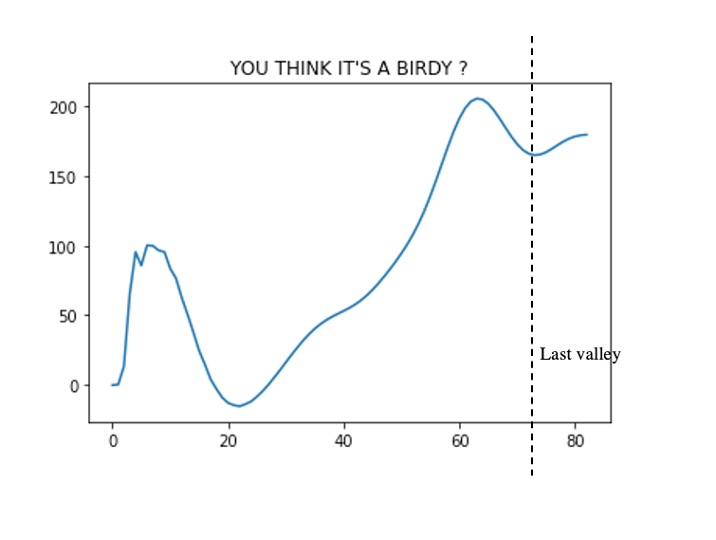
\includegraphics[width=0.7\textwidth]{figures/pitch-rise.jpg}
    \caption{``You think it's a birdy?''}
    \label{fig:rise-example}
\end{figure}

Figure~\ref{fig:rise-sp} and \ref{fig:rise-cl} show the proportion of final rise, as identified by the algorithm. As we can see, there is no difference in the proportion of rises among speech acts. 

\begin{figure}[H]
    \centering
    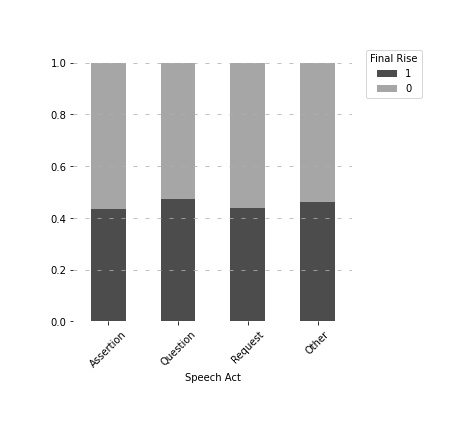
\includegraphics[width=0.7\textwidth]{figures/rise-sp.jpg}
    \caption{Proportion of utterances with final rise across different speech acts}
    \label{fig:rise-sp}
\end{figure}


\begin{figure}[H]
    \centering
    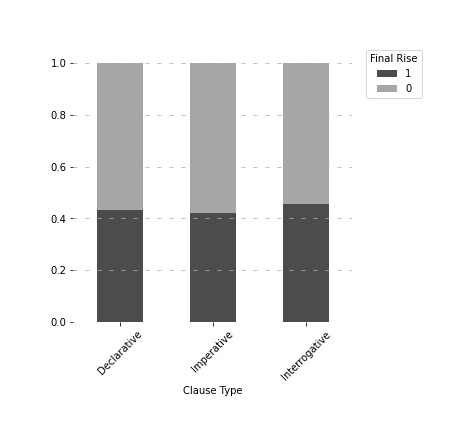
\includegraphics[width=0.7\textwidth]{figures/rise-cl.jpg}
    \caption{Proportion of utterances with final rise across different clause types}
    \label{fig:rise-cl}
\end{figure}

But if we look into sub-categories of interrogatives, we can see that the proportion of final rise is much higher with polar interrogatives than with declaratives. 
\begin{figure}[H]
    \centering
    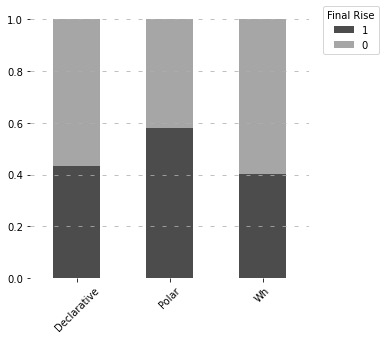
\includegraphics[width=0.7\textwidth]{figures/pitch-polardecwh.jpg}
    \caption{Proportion of declaratives, \twh{} and polar interrogatives with final rise}
    \label{fig:rise-int}
\end{figure}

These results seem to suggest that the presence of final rise might not be informative of the speech act of the sentence, unless morpho-syntactic features like subject-auxiliary inversion is also present. However, this could be a result of the algorithm I applied here, and do not reflect the pattern of the data. I plan to hand annotate more cases in the future to have more reliable data.

\section{Learning clause type categories with prosody}\label{sec:prosody:model}


\begin{minipage}[b]{0.45\linewidth}
\begin{figure}[H]
\begin{center}
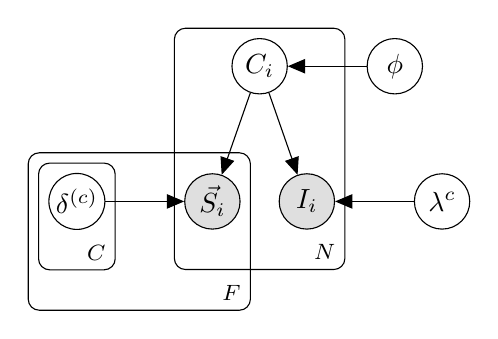
\begin{tikzpicture}
\node[latent] (c) {$C_{i}$};
\node[obs, below=of c, xshift=-0.6cm] (s) {$\vec{S_{i}}$};
\node[obs, below=of c, xshift=0.6cm] (i) {$I_{i}$};
\node[latent, right=of i] (lambda) {$\lambda^{c}$};
%\node[const, right=of lambda] (eta) {$\eta$};
\node[latent, right=of c] (phi) {$\phi$};
%\node[const, right=of phi] (beta) {$\beta$};
\node[latent, left=of s] (delta) {$\delta^{(c)}$};
%\node[const, left=of delta] (gamma) {$\gamma$};


\edge {phi}{c};
\edge {c}{s};
\edge {delta}{s};
%\edge {beta}{phi};
%\edge {gamma}{delta};
\edge {lambda, c}{i};
%\edge {eta}{lambda};


\plate {nutt}{(c)(s)(i)}{$N$};
\plate {cvalue}{(delta)}{$C$};
\plate {fvalue}{(cvalue)(s)}{$F$};
%\plate {fvalue}{(gamma)(delta)(s)(cvalue)}{$F$};
\end{tikzpicture}
\end{center}
%\caption{Hierarchical model with all parameters specified}\label{fg:model}
\end{figure}
\end{minipage}
\hspace{0.6cm}
\begin{minipage}[b]{0.45\linewidth}
\begin{figure}[H]
\begin{center}
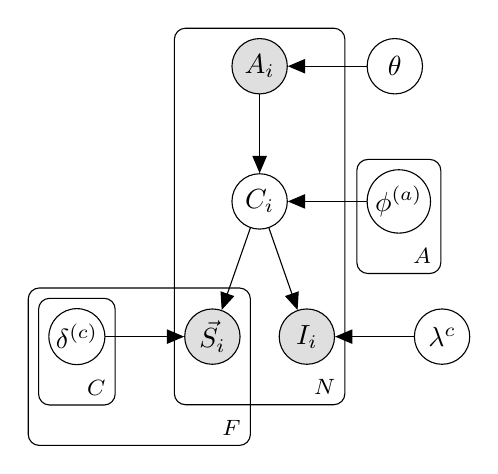
\begin{tikzpicture}
\node[obs] (a) {$A_{i}$};
\node[latent, right=of a] (theta) {$\theta$};
%\node[const, right=of theta] (alpha) {$\alpha$};
\node[latent, below=of a] (c) {$C_{i}$};
\node[obs, below=of c, xshift=-0.6cm] (s) {$\vec{S_{i}}$};
\node[obs, below=of c, xshift=0.6cm] (l) {$I_{i}$};
\node[latent, right=of l] (lambda) {$\lambda^{c}$};
%\node[const, right=of lambda] (eta) {$\eta$};
\node[latent, right=of c] (phi) {$\phi^{(a)}$};
%\node[const, right=of phi] (beta) {$\beta$};
\node[latent, left=of s] (delta) {$\delta^{(c)}$};
%\node[const, left=of delta] (gamma) {$\gamma$};

\edge {theta}{a};
%\edge {alpha}{theta};
\edge {phi, a}{c};
\edge {delta, c}{s};
%\edge {beta}{phi};
%\edge {gamma}{delta};
\edge {c,lambda}{l};
%\edge {eta}{lambda};


\plate {nutt}{(a)(c)(s)(l)}{$N$};
\plate {avalue}{(phi)}{$A$};
\plate {cvalue}{(delta)}{$C$};
\plate {fvalue}{(delta)(s)(cvalue)}{$F$};
\end{tikzpicture}
\end{center}
%\caption{Hierarchical model with all parameters specified}\label{fg:model}
\end{figure}
\end{minipage}

\begin{equation}\label{postC}
\begin{split}
p(c_{i}| c_{-i}, \vec{a}, \beta, \vec{S_{i}}, \delta, \gamma, l_{i}, \lambda, \eta) = &
\frac{p(\vec{S_{i}}| \vec{c}, \delta, \gamma)\ p(l_{i} |\vec{c},\lambda, \eta)\ p(c_{i}|\beta, c_{-i}, \vec{a})}{\Sigma_{c_{i}'}p(\vec{S_{i}}| \vec{c'}, \delta, \gamma)\ p(l_{i} |\vec{c'},\lambda, \eta)\ p(c_{i}'|\beta, c_{-i}, \vec{a})}\\
=& \frac{ \prod_{F}\frac{\gamma_{0}+n_{s^{F, c_{i}}_{i}}}{2r_{0}+n_{c^{F}_{i}}}%S
\frac{\eta_{0}+n_{l_{i}}^{c_{i}}}{2\eta_{0}+n_{c_{i}}}%L
\frac{\beta_{0}+n_{c_{i}}^{a_{i}}}{4\beta_{0}+n_{a_{i}}}%C
}%分子
{\sum_{c'_{i}}\prod_{F}\frac{\gamma_{0}+n^{F, c'_{i}}_{s_{i}}}{2r_{0}+n^{F}_{c'_{i}}}%S
\frac{\eta_{0}+n_{l_{i}}^{c'_{i}}}{2\eta_{0}+n_{c'_{i}}}%L
\frac{\beta_{0}+n_{c'_{i}}^{a_{i}}}{4\beta_{0}+n_{a_{i}}} %C
}%分母
\end{split}
\end{equation}

The data for this model were taken from the annotated dataset reported in Section~\ref{sec:engcl:corpus}. The labels of speech acts and morpho-syntactic observations were used as input to the models, and the true labels of clause type were used to evaluate the performance of the models. As the learners need to use the surface features of sentences to learn about clause-level properties, instead of one-noun utterances or utterances of only injectives, we eliminated from the dataset sentences that do not contain a verb or an auxiliary. In total, $3366$  sentences were fed into the models.


Overall, the \dlearnerabbr{} model fails to identify the clause type clustering in English, and fails to identify the characteristic morpho-syntactic properties for these clause types. 

\revise{Zooming in on the clusters identified by the models, I found that simulations with around 80\% noise cannot successfully identify all three clusters correctly while simulations with 70\% noise level can, even though the adjusted rand scores of these two levels are roughly the same. At 80\%, we can see that the \plearnerabbr{} reverts back to the performance of the \dlearnerabbr{} in that it fails to identify a cluster for declaratives (Figure~\ref{fig:heatmap-prosody}). Similar to the \dlearnerabbr{} model, the cluster containing most imperatives also contains many declaratives (\ref{fig:heatrev-prosody}). }

\begin{figure}[H]
\begin{minipage}[b]{0.45\linewidth}	
    \centering
    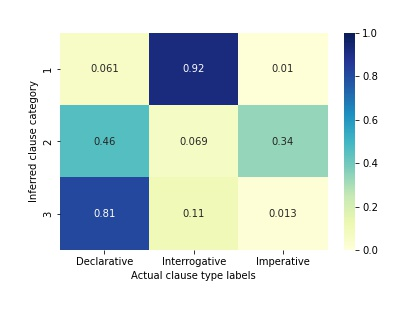
\includegraphics[width=1.2\textwidth]{figures/baseline-heatmap-bu.jpg}
\end{minipage}
\begin{minipage}[b]{0.45\linewidth}	
\centering
    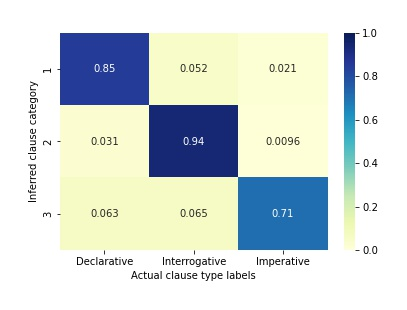
\includegraphics[width=1.2\textwidth]{figures/target-heatmap-bu.jpg}
\end{minipage}
    \caption{The proportion of \diis{} in each of the three clusters identified by the \dlearnerabbr{} (left) and the \plearnerabbr{} model (right). }
    \label{fig:heatmap-prosody}
\end{figure}

\begin{figure}[H]
\begin{minipage}[b]{0.45\linewidth}	
    \centering
    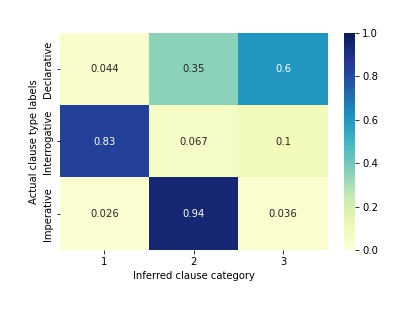
\includegraphics[width=1.2\textwidth]{figures/baseline-heatrev-bu.jpg}
\end{minipage}
\begin{minipage}[b]{0.45\linewidth}	
    \centering
    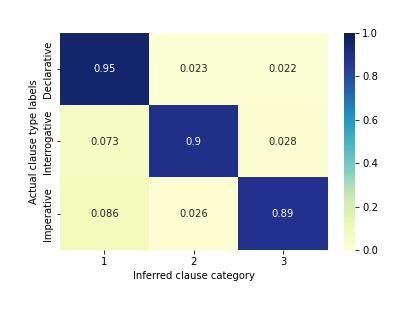
\includegraphics[width=1.2\textwidth]{figures/target-heatrev-bu.jpg}
\end{minipage}   
    \caption{The proportion of actual \diis{} clustered in one category as identified by the \dlearnerabbr{} (right) and \plearnerabbr{} (left) model with prosody respectively}
    \label{fig:heatrev-prosody}
\end{figure}



\revise{The morpho-syntactic profile of different simulations further shows that at 80\% noise level, the \plearnerabbr{} and \dlearnerabbr{} model behave similarly, as both fail to identify the property [$-$ subject] for imperatives (Figure~\ref{fig:noisy80-syncluster}). In contrast, with 70\% noise level the model can still find the right morpho-syntactic features for interrogatives and imperatives (Figure~\ref{fig:noisy70-syncluster}).} 

\begin{figure}[H]
    \centering
    \includegraphics[width=1\textwidth]{figures/baseline-syncluster-bu.jpg}
    \caption{\revise{The morpho-syntactic profile of each cluster in simulations (Cluster 1 $\sim$ Imperatives, Cluster 2 $\sim$ Interrogatives, Cluster 3 $\sim$ Declaratives).}}
    \label{fig:baseline-syncluster-prosody}
\end{figure}

\begin{figure}[H]
    \centering
    \includegraphics[width=1\textwidth]{figures/target-syncluster-bu.jpg}
    \caption{\revise{The morpho-syntactic profile of each cluster in simulations with 70\% noise in speech act information (Cluster 1 $\sim$ Interrogatives, Cluster 2 $\sim$ Imperatives, Cluster 3 $\sim$ Declaratives).}}
    \label{fig:target-syncluster-prosody}
\end{figure}

Results from our simulations suggest that morphosyntax is not sufficient to solve the clustering problem, and a small amount of pragmatic information is necessary.


\section{Conclusion}
\label{sec:prosody:discussion}
Cross-linguistically, pitch rises tend to signal questions and pitch falls signal assertions; and some argue that this universality reflects the innate knowledge that high pitch connects to the speech act of questioning (\cite{ohala1984,gussenhovenchen2000,gussenhoven2002} among others). If children are armed with the knowledge that questions tend to be associated with rising contours, they might expect rising contours to be somewhat correlated with the act of asking a question. But just as not all interrogatives have subject-auxiliary inversion, not all questions have final rises. With preliminary data, I found that parents do not use final rises more often with questions, but polar interrogatives have more final rises than other types of speech acts and clause types, including \twh-interrogatives and declaratives. It is hard to make sense of how children could take advantage of the prosodic data, since the correlation between final rise is not with the questioning speech act, but with a specific type of interrogative. 


\chapter{Learning speech act categories}
\label{chap:eng-sp}


Learners of both (perhaps all) languages face a further difficulty. Besides their main function of eliciting information, interrogative clauses can also be used to fulfill a range of other conventional functions. Test questions like (\ref{bg-prag:test}) do not present the asker as lacking information; parents can use questions like (\ref{bg-prag:ped}) to teach children object labels; indirect requests like (\ref{bg-prag:req}) are not genuinely soliciting information; and rhetorical questions act similar to assertions (\ref{bg-prag:rhe}). Such uses of interrogatives might mask the association of interrogatives with information-seeking speech acts. Additionally, other clause types like declaratives can be used as questions (e.g. rising declaratives, \citealt{gunlogson2004,gunlogson2008,jeong2018,rudin2018}). All these are potential sources of noise in the input with respect to the mapping between form and function.

\bex{bg-prag:types}
\bxl\label{bg-prag:test}
What is H$_{2}$O?		\hfill \tit{Test}
\ex \label{bg-prag:ped}
What's this?	\hfill \tit{Pedagogy}
\exl
\eex

\bex{}
\bxl\label{bg-prag:req}
Can you pass the salt?			\hfill \tit{Request}
\ex \label{bg-prag:rhe}
Are you crazy?	\hfill \tit{Rhetorical}
\exl
\eex


Common to all the functions listed above is the fact that in a conversation, questions expect responses (\citealt{duncan1972turn}). In turn-taking theory, questions usually mark the turn-transition points: after a question, the current speaker yields their turn and appoint the next speaker while the other participants of the conversation would pick up the turn by answering the question (\citealt{kendon1967gaze, argyle1972gaze, levinson1983, tice2011turn} among others, see \citealt{enfield2010} for a survey).  Additionally, questions are argued to set up the topics and issues in a conversation (\citealt{roberts2012,farkasbruce2010}), and speakers could use questions to keep track of where they are in a conversation. Therefore, despite the fact that questions can be used to fulfill many functions, the role of questions in a conversation seems to be clear: speakers use questions to solicit responses and set up topics for discussion. If children are sensitive to signals of response expectations or topic settings, they could make use of that information to identify questions, and, in turn, interrogatives. 
%As mentioned above, combining syntactic and prosodic information may explain some mismatches, as with the case of rising declaratives. Other syntactic markers might be helpful as well: many have noted that interrogatives that function like imperatives tend to take specific forms such as having modals like (\ref{bg-prag:req}), or \tit{why don't} and \tit{why not} interrogatives (i.e. \tit{whimperatives}, \citealt{sadock1974, green1975whimp}).


we will annotate the social function of each utterance. Our preliminary results in Fig.~\ref{fig:uttgoals} show that this prediction is borne out: parents tend to use questions to direct infants’ attention to new objects in their surrounding, while assertions are used to teach and express opinions.

\begin{table}[H]
\begin{center}
\begin{tabular}{c|p{6cm}|c}
\hline
Social Function&Explanation	&\tit{Example}\\
\hline
\hline
Attention& Direct attention to new object&\tit{Alex, Look!}\\
\hline
Negotiating & Negotiating about carrying out an action	&\tit{You read it to mommy.}\\
\hline
Teaching& Teaching the child about something or how to do things &\tit{What’s that (pointing to a bumblebee)?}\\
\hline
Discussing & Exchanging information but not for pedagogical purposes &\tit{Do you like scratchy cat kisses?}\\
\hline
Verbal Routines& Routines in social situations/games &\tit{Ready? Go!}\\
\hline
Emoting& Expressing emotions like excitement &\tit{Yay!}\\
\hline
Imitating & Imitating sounds, repeating others' utterances &\tit{vroom vroom!}\\
\hline
Meta-communication & Seeking clarification, confirmation, acknowledgement of another utterance/action	&\tit{ (after Alex makes some noise) What?}\\
\hline
\end{tabular}
\end{center}
\label{code:social}
\vspace{-4ex}
\caption{ Types of social functions of parents’ utterances}
\end{table}



%\vspace{-3ex}
%\noindent 
The other property of interest is that they expect responses. For conversations with pre-linguistic infants, this may mean that parents wait longer after questions for a response. Thus, in this project, we plan to measure the length of pause between parents’ consecutive utterances like (\ref{code-prag:pause}). To do so, we will first extract the consecutive turn sequences in parents’ speech. Following \cite{reimchen2017}, we define such sequences as a sequence of utterances spoken by the same speaker on the same topic. Within the sequences, we will measure the length of pauses between utterances, and see if parents pause longer after questions than after assertions. Moreover, we will code whether a question in the sequence is followed by another question, since \cite{reimchen2017} observe that parents to 14-month-olds tend to follow questions with another question. Our preliminary results show that parents are equally likely to ask another question as they are to answer their own questions, but parents tend to pause longer after questions (mean $= 1861ms$, Fig.~\ref{fg:pauses}) than assertions (mean $= 1216ms; t(347) = 2.08, p <0.05$): parents wait for responses after asking a question but proceed with the conversation after an assertion. 




\bex{code-prag:pause}
%\bxl{}
\tbf{Consecutive turn sequence}\\ 
%Alex's mother: Who’s that? [pause: 1.086s] Is that the postman?	\hfill		
\bxl
\ex You can’t take your rake on the swing but you can [pause: 0.014s] You wanna take your big bird rake on the swing? 			\hfill \tsc{Assertion -Question}
\ex You don't wanna swing? [pause: 0.23s]	You don’t have to.	\hfill \tsc{Question-Assertion}
\ex Here you use this one. [pause: 0.033s] This one works better.	\hfill \tsc{Assertion-Assertion}
\exl
\eex


%\begin{figure}[H]
%\begin{center}
%	\includegraphics[width = 0.5\textwidth]{q-followup.png}
%	\caption{Duration of pause (ms) after each speech act}\label{fg:pauses}
%\end{center}
%\end{figure}


Another consequence of the response-expectation property of questions is that by the end of a question, the speaker tends to appoint the next speaker. A common device for turn allocation is eye gaze (\citealt{argyle1972gaze, kendon1967gaze,duncan1979gaze, rossano2009gaze}), so the \hypos{} predicts that parents would engage in longer eye contact after questions than other types of speech acts. To test this, we plan to annotate, on a second-by-second basis, parents' attentional behaviors toward the child using ELAN. The annotation will be done without reference to the transcript so that the annotator is not biased by the linguistic information of the scene. For each video, the annotators will first identify the segments of the video where the parent and the child are both visible on screen, and the parent’s focus of attention is identifiable via her visual focus or head/body orientation. Then for these segments, we will annotate whether the parent is attending to the child.  


\begin{figure}[H]
\label{fg:attention}
\begin{center}
	%\includegraphics[width =0.4\textwidth]{q-attention.png}
	\vspace{-6ex}
	\caption{Proportion of parents' looks to the child (preliminary results)}
\end{center}
\end{figure}


Fig.~\ref{fg:attention} shows the proportion of looks to the child before and after uttering a sentence in our pilot sample: when the utterance is a question, the proportion of looks to the child is higher ($0.47$) than when it is an assertion ($0.39; t(16) = 2.53, p <0.05$) or a request ($0.35; t(16)= 4.55, p<0.001$); in the post-utterance region, the proportion of looks to the child is higher when the utterance is a question ($0.53$) than when it is an assertion ($0.37; t(4) = 4.4, p<0.05$) or a request ($0.35; t(4) = 13.2, p<0.001$). These results suggest that the predictions of the \hypos{} are borne out: parents look at the child longer after questions. Thus, despite parents asking questions whose answers they know, the characteristic turn-changing properties of questions are observable in speech pauses and speaker attention. 



\subsubsection{Syntactic features}\label{prop-code:syn}
 \noindent\emph{For Study~1 (English)}:
We expect most interrogatives to have subject-auxiliary inversion, although there might be many exceptions. Thus, we plan to annotate the relative positions of the subject and auxiliary to empirically test this prediction. Our pilot results suggest that inversion is indeed the dominant pattern, with 92\% of the interrogative clauses having auxiliaries preceding the subject. 
\chapter{Conclusion and discussion}
\label{chap:discussion}

\section{Summary of findings}
In language after language, we find three clause types (\diis{}) that are dedicated to three speech acts (\aqrs{}). By 18 months old, children seem to be able to differentiate these clause types and associate them with their canonical speech act. To gain this ability, they need to identify the right categories of clauses (i.e.\ solve the clustering problem) and figure out what speech act they are canonically used for (i.e.\ solve the labeling problem). To solve the labeling problem, some speech act information must be available to the learner, but since there is the possibility of mismatches -- sentences used to perform speech acts that are not canonically associated with their clause types -- it is not immediately clear how useful it is for learners to be able to identify speech acts, if it is useful at all. Then, to solve the clustering problem, children surely need to pay attention to the surface morpho-syntactic features of each sentence in their input. But in the input that learners actually receive, many surface features might be absent or misleading. Again, it seems plausible that the availability of some information related to speech acts might be helpful to the learner, but this information too is potentially misleading, again due to cases where sentences are used to perform speech acts that are not canonically associated with their clause type.

This dissertation investigates how children figure out clause type categories. In particular, are the surface formal features of the sentences in the input sufficient for children to figure out the clustering of clause types? If not, is speech act information helpful for solving the clustering problem? And how might learners access such speech act information?

I addressed these questions computationally by simulating two learners, a \distlearner{} (\dlearnerabbr{}), and a \praglearner{} (\plearnerabbr{}). Both learners use the surface morpho-syntactic features of the input sentences to attempt to cluster sentences into three categories, i.e.\ to learn the clause type categories. But the \plearnerabbr{} additionally has access to some information about which speech act is performed by a sentence. I found that in English, the \dlearnerabbr{} model could identify interrogative clause but could not identify the other two clauses, but in Mandarin, this model cannot find any of the right categories. The \plearnerabbr{} model in both languages outperforms the \dlearnerabbr{}. In English, the \plearnerabbr{} model can find all three clause types; in Mandarin, the model has problem with imperative clauses. These results suggest that pragmatics is helpful, indeed crucial, to solve the clustering problem. 

But if the speech act information is useful for clause type learning, how do children figure out speech act information? Given that the way we generally identify a speech act is via its clause type, there is a potentially vicious circle here -- you need to identify a sentence's clause type to infer the speech act that is being performed, but you need to be able to infer speech act information to learn to identify clause types. How do learners avoid this circularity?

One way to break this circularity is to \tit{not} think of the learning of speech acts and clause types as two processes that need to happen sequentially, but as a joint learning process. It is likely that children learn to identify speech act and clause type in tandem and mutually informative ways.

To get one step closer to understanding and evaluating this joint learning hypothesis, I first addressed the question of how much speech act information children need to identify clause types. With the \plearnerabbr{} model, I simulated the learning of clause type with various degrees of noise in the speech act information. I showed that even if children can only perceive speech act information a small proportion of the time, they can still benefit from this information, as a noisy pragmatic percept is superior to no pragmatics at all. 

I then explored what kind of non-clause type cues for speech act information are present in the input. Even if children must rely on clause type information to figure out the speech acts, they could have access to additional information that is unrelated to clause typing, but is informative for recognizing speech act type. When speakers perform speech acts, because of the conventional functions of these speech acts on the discourse, the performance might be associated with certain socio-pragmatic features. For example, because of questions' response-elicitation function, we would expect pauses after questions. With prior knowledge about the functions of communication, and expectations about what questions do, children might able to use these socio-pragmatic features to figure out this speech act. If children have such expectations, could they find anything in the input? 

I explored three cues that could potentially differentiate questions from other speech acts: prosody, pauses, and direct eye gaze. I found that parents do not use final rises more often with questions, but that polar interrogatives have more final rises than other types of speech acts and clause types, including \twh-interrogatives and declaratives. However, due to the limitation of the pitch identification algorithm, these results are still preliminary, and we need manually annotated pitch data to draw further conclusions. Moreover, parents tend to pause longer after questions, and attend to the child more when asking questions. Therefore it is in principle plausible that there are some socio-pragmatic features that children can use, in addition to their growing knowledge of clause types to infer the speech act category of an utterance. This little bit of information about speech act could then be used to provide enough pragmatic information that the child needs in order to get the clause type clusters identified accurately.

\section{The pragmatic syntactic bootstrapping hypothesis}

When examined separately, the learning of clause types and the learning of speech acts share many similarities. 
%The learning of clause types seem to parallel with the learning problems typically associated with the semantic bootstrapping hypothesis, and the learning of speech act categories seem to parallel to some degree to the problems addressed by the syntactic bootstrapping hypothesis. Let's look at them one by one. 


The clause type categories are abstract formal features of a sentence related to a variety of surface forms, none of which is obligatorily present and many of which can occur in sentences with a different clause-type feature. While in principle the surface formal features could be sufficient, this dissertation showed that they in fact fall short. To compensate for this insufficiency, learners can use the speech act information -- which is systematically related to clause types -- to learn to identify clause types and which surface features are relevant for clause typing.

%Leaving aside the nature of speech act categories for now, but they are also not directly observable from the input, same as clause types, and need to be inferred. 
Speech acts are abstract pragmatic/semantic/conceptual categories. As we have seen in Chapter~\ref{chap:eng-sp}, speech act categories are related to a variety of human behaviors (e.g. pauses and eye gaze), none of which are obligatorily present (you don't \emph{need} to pause after a question) and many of which can occur when performing other speech act categories. While I showed that the features are correlated with the use of questions, it is likely that the learners use the clause type information --- which is systematically related to speech acts --- to inform how they infer speech act types.

In both learning processes, one source of information could bridge the gap between the learners' input and the abstract category they need to acquire, because of the robust correlation between the major clause types and the major speech act types across languages. 

But as I have discussed throughout this dissertation, when we put these two learning processes together, our first impression is that there is a chicken-and-egg problem: the learner needs speech act information to learn clause types, but they also needs clause types to learn speech act information. To break this vicious cycle, \hypos{} proposes that the learner has to learn the two in tandem:

\begin{exe}\ex\label{ex:prag-syn-hypo}
\tbf{The \hypos{}}:\\
Children learn to identify speech acts and clause types in tandem and mutually informative ways: children learn to identify clause types by tracking formal regularities in conjunction with their growing knowledge of speech acts and its associated social pragmatic cues; similarly, they identify speech acts by tracking social pragmatic cues in conjunction with their growing understanding of the syntax of clause types. 
\end{exe} 

\begin{comment}


\bex{}
\ex
\begin{tikzpicture}[level distance=60pt]
\tikzset{every tree node/.style={align=center,anchor=north, font=\scriptsize}}
%}}
\tikzset{level 1/.style={level distance=35pt}}
\tikzset{level 2/.style={sibling distance=35pt}}
%\tikzset{level 3/.style={sibling distance=-6pt}}
%\tikzset{level 4+/.style={sibling distance=-6pt}}
\Tree
[. {Sentential force} 
	[. {Clause type features\\ ([\textpm int, imp])} 
		[. {Surface formal features} ]
		[. {Prosodic features} ]
	]
	[. {Speech act categories \\
	\aqrs{}} 
		
		[. {Prosodic features} ]
		[. {Social pragmatic features} ]
	]
]

\end{tikzpicture}
\eex
\end{comment}


In this dissertation, I have established (a) that the learning of clause types does not require perfect speech act information; thus, it is possible that children learn clause type information while still trying to figure out the speech act information. And, (b) that there are social pragmatic cues associated with the use of the speech act of questioning. So if a child is equipped with a theory of what questions do, in addition to an innate knowledge that there are speech act categories that are associated with clause types, they could potentially find the signals they need.

In future work, I plan to test the feasibility of the speech act bootstrapping hypothesis computationally. Figure~\ref{fg:model} shows the graphical model. 
  
\begin{figure}[H]
\centering
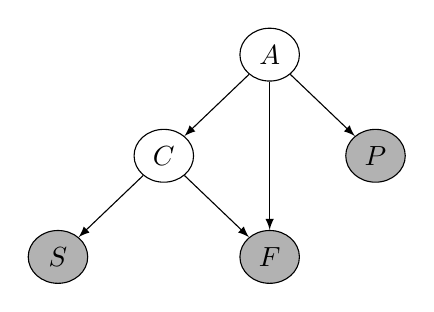
\begin{tikzpicture}[
  node distance= 0.8cm and 0.8cm,
  classnode/.style={draw,ellipse,text width=0.3cm,align=center},
  enode/.style={draw,ellipse,text width=0.2cm,align=center},
  obsnode/.style={draw,ellipse,text width=0.3cm,align=center, fill=black!30}
]
\node[classnode] (a) {$A$};
\node[obsnode, below right=of a] (p) {$P$};
\node[classnode, below left =of a] (c) {$C$};
\node[obsnode, below left=of c] (s) {$S$};
\node[obsnode, below right =of c] (f) {$F$};
%\node[enode, left=of c] (e) {$e$};
\path (a) edge[-latex] (p)
(a) edge[-latex] (c)
(c) edge[-latex] (s)
(c) edge[-latex] (f)
(a) edge[-latex] (f)
;
\end{tikzpicture}
\caption{Graphical Model}\label{fg:model}
\end{figure}

The question is then whether it is possible for a learner to use the expected social pragmatic cues to initially identify questions in their input, and use this speech act information to bootstrap the process of learning to identify the surface properties of interrogative clauses. The proposed model will (i) track the prosodic and pragmatic features of each utterance and infer the speech act that would generate these features; (ii) using knowledge of prosodic and syntactic features of each sentence, the model will be able to identify the clause type that would generate these features; and (iii) speech and clause type categories will influence each other. The advantage of such a learner is that it can exploit pragmatics to identify clause type indirectly via identifying the speech act, and exploit syntax to identify speech act indirectly via identifying the clause type. 

%%%%
\begin{comment}
Previously, \textcite{hacquardlidz2018} proposes the \hypos{} to address the learning of attitude verbs like \tit{think}. In their paper, the hypothesis is proposed for the learning of an abstract semantic property (the semantic class of an attitude verb) that is systematically related to (a) syntactic distribution and (b) pragmatic function. The \hypos{} is proposed to deal with the problem that observations of only the syntactic distribution or only the pragmatic function had the potential to mislead, so each was used to constrain the other. 

In our situation, the learners need to figure out two abstract categories, the clause types and the speech acts information, and the =two categories need to be learned in tandem. 

\tbf{The \hypos{}} (alternative):\\
Children learn to identify the sentential force of a sentence by observing the speech acts that the sentence is used to perform on the one hand, and observing the syntactic clause types in tandem and mutually informative ways: children learn to identify clause types by tracking formal regularities in conjunction with their growing knowledge of speech acts and its associated social pragmatic cues; similarly, they identify speech acts by tracking social pragmatic cues in conjunction with their growing understanding of the syntax of clause types. 

because of the systematic mapping between the three major clause types and the three major speech acts, 
The semantic bootstrapping hypothesis states that:
\begin{quote}
[T]he child uses the presence of \tit{semantic} entities such as ``thing,'' ``causal agent,'' ``true in past'' and ``predicate-argument relation'' to infer that the input contains tokens of the corresponding syntactic substantive universals such as \tit{noun}, \tit{subject}, \tit{auxiliary}, \tit{dominates} and so on.\\
\hspace*{\fill} \cite[407]{pinker1987} 
\end{quote}
\end{comment}
%%%%

%When putting these two together, it first appears that we might have a chicken-and-egg problem: 





%\begin{appendices}
 % % -*- mode: latex; coding: utf-8; fill-column: 72; -*-

\chapter{Clause Types and Speech Acts in English}%
\label{appx:engcl}

Three logistic regression models with each of the clause type as the dependent variable and the 8 morpho-syntactic features (the presence/absence of verbs and unknown functional item at preverbal position were excluded due to extremely low variance) as independent variables were performed, and the results are summarized in Table~\ref{tab:engcl:real-synstats}:


\begin{table}[H]
\begin{center}
\begin{tabular}{r|l|l|l}
\hline
 & Declaratives   & Interrogatives   & Imperatives \\
 & $\beta$  & $\beta$  & $\beta$ \\
 \hline\hline
constant & -1.7*** & -4.91*** & 1.21*** \\
\hline
Subject & 3.35*** & 1.08*** & -4.61*** \\
\hline
Verb Morphology & 1.01*** & 0.21  & -2.02*** \\
\hline
Auxiliary & 0.09  & 0.67*** & $-0.53{\cdot}$ \\
\hline
Subject-Aux Inversion & -4.2*** & 4.87*** & -1.52*** \\
\hline
Sentence-initial UFI & -2.59*** & 3.99*** & -2.38*** \\
\hline
Post-verbal UFI & -0.44  & -0.23  & $1.12{\cdot}$ \\
\hline \hline
\end{tabular}
\end{center}
\caption{Results from the three logistic regression models with each of the clause type as the dependent variable and the morpho-syntactic features as independent variables; asterisks represent the significance level: 0 ‘***’ 0.001 ‘**’ 0.01 ‘*’ 0.05 ‘$\cdot$’ 0.1 ‘ ’ 1}
\label{tab:engcl:real-synstats}
\end{table}%


% Local Variables:
% TeX-engine: xetex
% LaTeX-biblatex-use-Biber: t
% TeX-master: "../main"
% LocalWords: 
% End:


%\end{appendices}

%%%%%%%%%%%%%%%%%%%%%%%%%%%%%%%%%%%%%%%%%%%%%%%


\backmatter

\printbibliography

\end{document}

% Local Variables:
% TeX-engine: xetex
% LaTeX-biblatex-use-Biber: t
% TeX-master: t
% End:
